%==============================================================================
% Tento soubor použijte jako základ
% This file should be used as a base for the thesis
% Autoři / Authors: 2008 Michal Bidlo, 2022 Jaroslav Dytrych
% Kontakt pro dotazy a připomínky: sablona@fit.vutbr.cz
% Contact for questions and comments: sablona@fit.vutbr.cz
%==============================================================================
% kódování: UTF-8 (zmena prikazem iconv, recode nebo cstocs)
% encoding: UTF-8 (you can change it by command iconv, recode or cstocs)
%------------------------------------------------------------------------------
% zpracování / processing: make, make pdf, make clean
%==============================================================================
% Soubory, které je nutné upravit nebo smazat: / Files which have to be edited or deleted:
%   projekt-20-literatura-bibliography.bib - literatura / bibliography
%   projekt-01-kapitoly-chapters.tex - obsah práce / the thesis content
%   projekt-01-kapitoly-chapters-en.tex - obsah práce v angličtině / the thesis content in English
%   projekt-30-prilohy-appendices.tex - přílohy / appendices
%   projekt-30-prilohy-appendices-en.tex - přílohy v angličtině / appendices in English
%==============================================================================
%\documentclass[]{fitthesis} % bez zadání - pro začátek práce, aby nebyl problém s překladem
%\documentclass[english]{fitthesis} % without assignment - for the work start to avoid compilation problem

\documentclass[zadani]{fitthesis} % odevzdani do IS VUT a/nebo tisk s barevnými odkazy - odkazy jsou barevné
%\documentclass[english,zadani]{fitthesis} % for submission to the IS VUT and/or print with color links - links are color
%\documentclass[zadani,print]{fitthesis} % pro černobílý tisk - odkazy jsou černé
%\documentclass[english,zadani,print]{fitthesis} % for the black and white print - links are black
%\documentclass[zadani,cprint]{fitthesis} % pro barevný tisk - odkazy jsou černé, znak VUT barevný
%\documentclass[english,zadani,cprint]{fitthesis} % for the print - links are black, logo is color
% * Je-li práce psaná v anglickém jazyce, je zapotřebí u třídy použít 
%   parametr english následovně:
%   If thesis is written in English, it is necessary to use 
%   parameter english as follows:
%      \documentclass[english]{fitthesis}
% * Je-li práce psaná ve slovenském jazyce, je zapotřebí u třídy použít 
%   parametr slovak následovně:
%   If the work is written in the Slovak language, it is necessary 
%   to use parameter slovak as follows:
%      \documentclass[slovak]{fitthesis}
% * Je-li práce psaná v anglickém jazyce se slovenským abstraktem apod., 
%   je zapotřebí u třídy použít parametry english a enslovak následovně:
%   If the work is written in English with the Slovak abstract, etc., 
%   it is necessary to use parameters english and enslovak as follows:
%      \documentclass[english,enslovak]{fitthesis}

% Základní balíčky jsou dole v souboru šablony fitthesis.cls
% Basic packages are at the bottom of template file fitthesis.cls
% zde můžeme vložit vlastní balíčky / you can place own packages here


% Pro seznam zkratek lze využít balíček Glossaries - nutno odkomentovat i níže a při kompilaci z konzoly i v Makefile (plnou verzi pro Perl, nebo lite)
% The Glossaries package can be used for the list of abbreviations - it is necessary to uncomment also below. When compiling from the console also in the Makefile (full version for Perl or lite)
%\usepackage{glossaries}
%\usepackage{glossary-superragged}
%\makeglossaries 

% Nastavení cesty k obrázkům
% Setting of a path to the pictures
%\graphicspath{{obrazky-figures/}{./obrazky-figures/}}
%\graphicspath{{obrazky-figures/}{../obrazky-figures/}}

%---rm---------------
\renewcommand{\rmdefault}{lmr}%zavede Latin Modern Roman jako rm / set Latin Modern Roman as rm
%---sf---------------
\renewcommand{\sfdefault}{qhv}%zavede TeX Gyre Heros jako sf
%---tt------------
\renewcommand{\ttdefault}{lmtt}% zavede Latin Modern tt jako tt

% vypne funkci šablony, která automaticky nahrazuje uvozovky,
% aby nebyly prováděny nevhodné náhrady v popisech API apod.
% disables function of the template which replaces quotation marks
% to avoid unnecessary replacements in the API descriptions etc.
\csdoublequotesoff

\usepackage{url}
\usepackage{caption}
\usepackage{enumitem}
\captionsetup[figure]{justification=centering}
\nocite{*}

% =======================================================================
% balíček "hyperref" vytváří klikací odkazy v pdf, pokud tedy použijeme pdflatex
% problém je, že balíček hyperref musí být uveden jako poslední, takže nemůže
% být v šabloně
% "hyperref" package create clickable links in pdf if you are using pdflatex.
% Problem is that this package have to be introduced as the last one so it 
% can not be placed in the template file.
\ifWis
\ifx\pdfoutput\undefined % nejedeme pod pdflatexem / we are not using pdflatex
\else
  \usepackage{color}
  \usepackage[unicode,colorlinks,hyperindex,plainpages=false,pdftex]{hyperref}
  \definecolor{hrcolor-ref}{RGB}{223,52,30}
  \definecolor{hrcolor-cite}{HTML}{2F8F00}
  \definecolor{hrcolor-urls}{HTML}{092EAB}
  \hypersetup{
	linkcolor=hrcolor-ref,
	citecolor=hrcolor-cite,
	filecolor=magenta,
	urlcolor=hrcolor-urls
  }
  \def\pdfBorderAttrs{/Border [0 0 0] }  % bez okrajů kolem odkazů / without margins around links
  \pdfcompresslevel=9
\fi
\else % pro tisk budou odkazy, na které se dá klikat, černé / for the print clickable links will be black
\ifx\pdfoutput\undefined % nejedeme pod pdflatexem / we are not using pdflatex
\else
  \usepackage{color}
  \usepackage[unicode,colorlinks,hyperindex,plainpages=false,pdftex,urlcolor=black,linkcolor=black,citecolor=black]{hyperref}
  \definecolor{links}{rgb}{0,0,0}
  \definecolor{anchors}{rgb}{0,0,0}
  \def\AnchorColor{anchors}
  \def\LinkColor{links}
  \def\pdfBorderAttrs{/Border [0 0 0] } % bez okrajů kolem odkazů / without margins around links
  \pdfcompresslevel=9
\fi
\fi
% Řešení problému, kdy klikací odkazy na obrázky vedou za obrázek
% This solves the problems with links which leads after the picture
\usepackage[all]{hypcap}
\usepackage{algorithm}
\usepackage{algpseudocode}

% Informace o práci/projektu / Information about the thesis
%---------------------------------------------------------------------------
\projectinfo{
  %Prace / Thesis
  project={BP},            %typ práce BP/SP/DP/DR  / thesis type (SP = term project)
  year={2023},             % rok odevzdání / year of submission
  date=\today,             % datum odevzdání / submission date
  %Nazev prace / thesis title
  title.cs={Aplikace genetického programování},  % název práce v češtině či slovenštině (dle zadání) / thesis title in czech language (according to assignment)
  title.en={Genetic Programming Applications}, % název práce v angličtině / thesis title in english
  %title.length={14.5cm}, % nastavení délky bloku s titulkem pro úpravu zalomení řádku (lze definovat zde nebo níže) / setting the length of a block with a thesis title for adjusting a line break (can be defined here or below)
  %sectitle.length={14.5cm}, % nastavení délky bloku s druhým titulkem pro úpravu zalomení řádku (lze definovat zde nebo níže) / setting the length of a block with a second thesis title for adjusting a line break (can be defined here or below)
  %dectitle.length={14.5cm}, % nastavení délky bloku s titulkem nad prohlášením pro úpravu zalomení řádku (lze definovat zde nebo níže) / setting the length of a block with a thesis title above declaration for adjusting a line break (can be defined here or below)
  %Autor / Author
  author.name={Tadeáš},   % jméno autora / author name
  author.surname={Kachyňa},   % příjmení autora / author surname 
  %author.title.p={Bc.}, % titul před jménem (nepovinné) / title before the name (optional)
  %author.title.a={Ph.D.}, % titul za jménem (nepovinné) / title after the name (optional)
  %Ustav / Department
  department={UPSY}, % doplňte příslušnou zkratku dle ústavu na zadání: UPSY/UIFS/UITS/UPGM / fill in appropriate abbreviation of the department according to assignment: UPSY/UIFS/UITS/UPGM
  % Školitel / supervisor
  supervisor.name={Michal},   % jméno školitele / supervisor name 
  supervisor.surname={Bidlo},   % příjmení školitele / supervisor surname
  supervisor.title.p={Ing. },   %titul před jménem (nepovinné) / title before the name (optional)
  supervisor.title.a={Ph.D.},    %titul za jménem (nepovinné) / title after the name (optional)
  % Klíčová slova / keywords
  keywords.cs={stromové genetické programování, lineární genetické programování, evoluční algoritmy, langtonův mravenec}, % klíčová slova v českém či slovenském jazyce / keywords in czech or slovak language
  keywords.en={tree-based genetic programming, linear genetic programming,  evolutionary algorithms, langton's ant}, % klíčová slova v anglickém jazyce / keywords in english
  %keywords.en={Here, individual keywords separated by commas will be written in English.},
  % Abstrakt / Abstract
  abstract.cs={
Tato práce se věnuje problematice úlohy Langtonova mravence a~využití stromového a~lineárního genetického programování jako metod pro řešení tohoto problému. Langtonův mravenec je abstraktní matematický model, jenž využívá jednoduchých pravidel k~pohybu mravence po dvoudimenzionální mřížce. Úkolem je sesbírat všechnu potravu v~co nejmenším počtu kroků. Cílem práce je tedy aplikace výše dvou zmíněných technik na vybrané instance tohoto problému, následné provedení experimentů a statistické vyhodnocení včetně porovnání výsledků s~těmi dostupnými v~literatuře. Mimo to bude cílem dané metody optimalizovat různými vylepšeními pro dosáhnutí co nejlepších výsledků. },
  % abstrakt v českém či slovenském jazyce / abstract in czech or slovak language
  abstract.en={This thesis deals with the problem of the Langton's artificial ant task and the use of tree-based and linear genetic programming as methods for solving this problem. Langton's ant is an abstract mathematical model that uses simple rules to move an ant along a two-dimensional grid. The task is to collect all the food in as few steps as possible. The goal of the thesis is the application of the two techniques mentioned above to selected instances of this problem, subsequent experimentation and statistical evaluation, including a comparison of the results with those available in the literature. In addition, the aim will be to optimize the given methods with various improvements to achieve the best possible results.}, % abstrakt v anglickém jazyce / abstract in english
  %abstract.en={An abstract of the work in English will be written in this paragraph.},
  % Prohlášení (u anglicky psané práce anglicky, u slovensky psané práce slovensky; u projektové praxe lze zakomentovat) / Declaration (for thesis in english should be in english; for project practice can be commented out)
  declaration={Prohlašuji, že jsem tuto bakalářskou práci vypracoval samostatně pod vedením pana Ing. Michala Bidla, PhD.
Uvedl jsem všechny literární prameny, publikace a další zdroje, ze kterých jsem čerpal.},
  %declaration={I hereby declare that this Bachelor's thesis was prepared as an original work by the author under the supervision of Mr. X
% The supplementary information was provided by Mr. Y
% I have listed all the literary sources, publications and other sources, which were used during the preparation of this thesis.},
  % Poděkování (nepovinné, nejlépe v jazyce práce; nechcete-li, zakomentujte pro skrytí nadpisu) / Acknowledgement (optional, ideally in the language of the thesis; comment out for hiding including heading)
  acknowledgment={Tímto bych rád poděkoval Ing. Michalu Bidlovi, PhD. za odborné vedení práce, nápomocnost a věnovaný čas při konzultacích.},
  %acknowledgment={Here it is possible to express thanks to the supervisor and to the people which provided professional help
%(external submitter, consultant, etc.).},
  % Rozšířený abstrakt (cca 3 normostrany) - lze definovat zde nebo níže / Extended abstract (approximately 3 standard pages) - can be defined here or below
  %extendedabstract={Do tohoto odstavce bude zapsán rozšířený výtah (abstrakt) práce v českém (slovenském) jazyce.},
  %extabstract.odd={true}, % Začít rozšířený abstrakt na liché stránce? / Should extended abstract start on the odd page?
  %faculty={FIT}, % FIT/FEKT/FSI/FA/FCH/FP/FAST/FAVU/USI/DEF
  faculty.cs={Fakulta informačních technologií}, % Fakulta v češtině - pro využití této položky výše zvolte fakultu DEF / Faculty in Czech - for use of this entry select DEF above
  faculty.en={Faculty of Information Technology}, % Fakulta v angličtině - pro využití této položky výše zvolte fakultu DEF / Faculty in English - for use of this entry select DEF above
  department.cs={Ústav matematiky}, % Ústav v češtině - pro využití této položky výše zvolte ústav DEF nebo jej zakomentujte / Department in Czech - for use of this entry select DEF above or comment it out
  department.en={Institute of Mathematics} % Ústav v angličtině - pro využití této položky výše zvolte ústav DEF nebo jej zakomentujte / Department in English - for use of this entry select DEF above or comment it out
}

% Rozšířený abstrakt (cca 3 normostrany) - lze definovat zde nebo výše / Extended abstract (approximately 3 standard pages) - can be defined here or above
%\extendedabstract{Do tohoto odstavce bude zapsán výtah (abstrakt) práce v českém (slovenském) jazyce.}
% Začít rozšířený abstrakt na liché stránce? / Should extended abstract start on the odd page?
%\extabstractodd{true}

% nastavení délky bloku s titulkem pro úpravu zalomení řádku - lze definovat zde nebo výše / setting the length of a block with a thesis title for adjusting a line break - can be defined here or above
%\titlelength{14.5cm}
% nastavení délky bloku s druhým titulkem pro úpravu zalomení řádku - lze definovat zde nebo výše / setting the length of a block with a second thesis title for adjusting a line break - can be defined here or above
%\sectitlelength{14.5cm}
% nastavení délky bloku s titulkem nad prohlášením pro úpravu zalomení řádku - lze definovat zde nebo výše / setting the length of a block with a thesis title above declaration for adjusting a line break - can be defined here or above
%\dectitlelength{14.5cm}

% řeší první/poslední řádek odstavce na předchozí/následující stránce
% solves first/last row of the paragraph on the previous/next page
\clubpenalty=10000
\widowpenalty=10000

% checklist
\newlist{checklist}{itemize}{1}
\setlist[checklist]{label=$\square$}

% Kompilace po částech (rychlejší, ale v náhledu nemusí být vše aktuální)
% Compilation piecewise (faster, but not all parts in preview will be up-to-date)
% Další informace viz / For more information see https://www.overleaf.com/learn/latex/Multi-file_LaTeX_projects
% \usepackage{subfiles}

% Nechcete-li, aby se u oboustranného tisku roztahovaly mezery pro zaplnění stránky, odkomentujte následující řádek / If you do not want enlarged spacing for filling of the pages in case of duplex printing, uncomment the following line
% \raggedbottom

\begin{document}
  % Vysazeni titulnich stran / Typesetting of the title pages
  % ----------------------------------------------
  \maketitle
  % Obsah
  % ----------------------------------------------
  \setlength{\parskip}{0pt}
    \setcounter{tocdepth}{2}
  {\hypersetup{hidelinks}\tableofcontents}
  
  % Seznam obrazku a tabulek (pokud prace obsahuje velke mnozstvi obrazku, tak se to hodi)
  % List of figures and list of tables (if the thesis contains a lot of pictures, it is good)
  % \ifczech
  %   \renewcommand\listfigurename{Seznam obrázků}
  % \fi
  % \ifslovak
  %   \renewcommand\listfigurename{Zoznam obrázkov}
  % \fi
  % {\hypersetup{hidelinks}\listoffigures}
  
  \ifczech
    \renewcommand\listtablename{Seznam tabulek}
  \fi
  \ifslovak
    \renewcommand\listtablename{Zoznam tabuliek}
  \fi
  % {\hypersetup{hidelinks}\listoftables}

  % Seznam zkratek / List of abbreviations
  %\ifczech
  %  \renewcommand*\glossaryname{Seznam zkratek}%
  %  \renewcommand*\entryname{Zkratka}
  %  \renewcommand*\descriptionname{Význam}
  %\fi
  %\ifslovak
  %  \renewcommand*\glossaryname{Zoznam skratiek}%
  %  \renewcommand*\entryname{Skratka}
  %  \renewcommand*\descriptionname{Význam}
  %\fi
  %\ifenglish
  %  \renewcommand*\glossaryname{List of abbreviations}%
  %  \renewcommand*\entryname{Abbreviation}
  %  \renewcommand*\descriptionname{Meaning}
  %\fi
  % Definice zkratek - z textu se odkazují např. \Gls{TF–IDF}
  % Definition of abbreviations - referred from the text e.g. \Gls{TF–IDF}
  %\newglossaryentry{TF–IDF}
  %{
  %  name={TF–IDF},
  %  description={Term Frequency-Inverse Document Frequency}
  %}
  % 
  %\setglossarystyle{superragged}
  %\printglossaries


  \ifODSAZ
    \setlength{\parskip}{0.5\bigskipamount}
  \else
    \setlength{\parskip}{0pt}
  \fi

  % vynechani stranky v oboustrannem rezimu
  % Skip the page in the two-sided mode
  \iftwoside
    \cleardoublepage
  \fi

  % Text prace / Thesis text
  % ----------------------------------------------
  \ifenglish
    \input{projekt-01-kapitoly-chapters-en}
  \else
    % ===================================================
% KAPITOLA 1 -- ÚVOD

\vspace{3cm}
\noindent \textbf{\large Seznam některých použitých zkratek}  \\
\begin{description}[wide=0\parindent]
    \item[GP] Genetické programování 
    \item[TGP] Stromové genetické programování 
    \item[LGP] Lineární genetické programování 
    \item[GA] Genetické algoritmy
    \item[ES] Evoluční strategie 
    \item[EP] Evoluční programování \\
\end{description}

\chapter{Úvod}\label{ch:1}

V~této práci se budu zabývat genetickým programováním a konkrétněji jeho dvěma variantami -- stromovým a lineárním. Tyto varianty budu následně aplikovat na vybrané instance zvoleného problému a porovnávat jejich efektivitu a schopnost najít co nejlepší řešení. 

Genetické programování (GP) je jednou z~několika programovacích technik spadajících pod evoluční algoritmy zpopularizovanou zejména americkým vědcem a matematikem J.~Kozou, který o~ní sepsal nemálo úspěšných publikací. Jedná se o~metodu strojového učení, kdy se každou iterací tohoto algoritmu přibližujeme více k~požadovanému řešení. Na počátku je inicializována populace náhodných jedinců, která je v~průběhu generací modifikována za pomocí genetických operátorů. Po každé generaci je populace ohodnocena tzv. fitness funkcí, která nám udává kvalitu jednotlivých řešení. Takto běží algoritmus do té doby, dokud není přerušen ukončovací podmínkou, nebo není nalezeno nejlepšího řešení. Díky své popularitě nabylo GP několika podob, aby bylo lépe aplikovatelné na různé problémy. Často se tyto varianty liší právě ve své reprezentaci.

Tato technika má v~reálném světě mnoho aplikací počínaje od návrhu inženýrských systémů, klasifikace a rozpoznávání obrázků, navrhování elektrických obvodů až třeba po návrh a řízení robotů. Mezi největší výhody GP patří objevení nových a nečekaných řešení, která by nemusela být tradičními metodami nalezena, flexibilita -- tedy schopnost adaptovat se na široké spektrum různorodých problémů, škálovatelnost na velmi komplexní problémy s~mnoha proměnnými nebo schopnost vypořádat se stochasticitou. 

Cílem této práce je porovnání dvou různých variant GP na vybraných instancích Langtonova mravence. Tato úloha představuje abstraktní matematický model, kdy se umělý mravenec snaží nalézt nejlepší cestu na dvojdimenzionální mřížce k~sesbírání potravy v~ideálně co nejmenším počtu kroků.  Mimo to se v~práci budu zabývat zefektivněním a modifikací již zavedených metod, např. genetických operátorů, k~nalezení lepších řešení. 

Obsah práce je rozdělen do kapitol následovně: 

\begin{itemize}
    \item V~\ref{ch:2}. kapitole je představeno stromové GP, vysvětlena základní terminologie pojící se s~tímto tématem, obecné koncepce aplikovatelné na všechny varianty GP a v~závěru kapitoly se nachází krátké srovnání s~ostatními evolučními algoritmy.
    \item V~\ref{ch:3}. kapitole je popsána varianta lineárního GP, její charakteristika a reprezentace, variační operátory včetně grafického znázornění a v~závěru srovnání se stromovým GP.
    \item V~\ref{ch:4}. kapitole jsou prezentovány výhody použití metody GP k řešení reálných problémů, následně je detailně představeno několik  aplikací.
    \item \ref{ch:5}. kapitola objasňuje úlohu Langtonova mravence a vlastní přístup k~jejímu řešení.
    \item \ref{ch:6}. kapitola se odkazuje na popis implementace obou variant GP na problému Langtonova mravence.
    \item V~\ref{ch:7}. kapitole je představen způsob experimentování, následné experimenty, jejich vyhodnocení, souhrnné zhodnocení a pojednání o dalších vylepšeních.
\end{itemize}

% ===================================================
% KAPITOLA 2 -- GENETICKÉ PROGRAMOVÁNÍ

\chapter{Genetické programování}\label{ch:2}
Tato kapitola se zabývá popisem stromového genetického programování a objasněním obecných konceptů aplikovatelných pro všechny varianty GP.  Taktéž tu je zmíněna a vysvětlena základní terminologie, která s touto technikou programování souvisí a bude potřebná pro porozumění dalších částí této práce. Ke konci kapitoly je provedeno krátké srovnání s dalšími známými evolučními algoritmy. Tato kapitola vychází především z následujících zdrojů~\cite{Brameier1998, eiben-2015B, EvoFitLectures, GenProg}. 

\begin{figure}[b!]
    \centering
    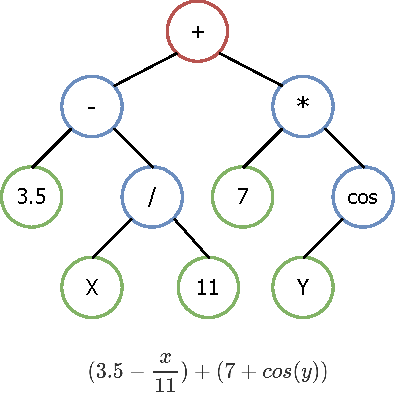
\includegraphics{obrazky-figures/tree.pdf}
    \caption{Reprezentace programu pomocí stromového GP a jeho ekvivalentního matematického zápisu. Barevně jsou zde zvýrazněny kořenový (červený), vnitřní (modré) a vnější (zelené) uzly.}
    \label{fig:tgp_representation}
\end{figure}

Genetické programování je jedna z~nejnovějších technik evolučních algoritmů založená na strojovém učení sloužící k~řešení netriviálních úloh za pomocí biologické evoluce reprezentující jednotlivá řešení jako stromové struktury, viz obr. \ref{fig:tgp_representation}. Jiným způsobem by se tato technika dala popsat následujícím citátem.
\vspace{0.2cm}
\begin{center}
\emph{How can computer learns to solve problems without being explicitly programmed? In other words, how can computers be made to do what is needed to be done, without being told exactly how to do it. -- Arthur Samuel (1959)}
\end{center}
\vspace{0.2cm}

Od ostatních evolučních algoritmů se liší nejen svou reprezentací, ale taky svou aplikací na velkou škálu různých problémů včetně optimalizace, predikce, kontroly řízení a datové analýzy. Má schopnost najít řešení, která jsou jednoduchá a zároveň efektivní a také kompetenci řešit problémy s~komplexními datovými strukturami a vícero objekty. V průběhu dalších let vznikly další varianty GP. Vyjma stromového je rozlišováno např. mezi lineárním~\cite{LGP}, kartézským~\cite{CGP}, zásobníkovým~\cite{SBGP} nebo gramatickou evolucí~\cite{wiki:Genetic_programming}.

Oblast GP byla poprvé představena v~80. letech americkým vědcem a matematikem Johnem Kozou. Byl to právě on, kdo aplikoval genetické algoritmy na jazyku LISP k~řešení velkého rozsahu různých problémů. Ačkoliv myšlenka zkombinovat genetické algoritmy a~počítačové programy tu už byla mnohem dříve~\cite{wiki:Genetic_programming}. Koza zároveň konstatuje, že je GP nejobecnějším paradigmatem strojového učení~\cite{NatSelectionGP}. Následně sepsal několik publikací o~této technice, ale byla to až série 4 knih s doprovodnými videi\footnote{Odkaz na první knihu ze série \uv{Genetic Programming: On the Programming of Computers by Means of Natural Selection} včetně doprovodných videí \url{http://gpbib.cs.ucl.ac.uk/gp-html/koza_book.html}}, díky níž se začala tato technika  v~průběhu 90. let postupně více upevňovat, dostávat se do podvědomí ostatním vědcům, a~to i díky každoročním konferencím, jež Koza v r. 1996 započal~\cite{wiki:Genetic_programming}. V r. 2010 představil Koza 76 výsledků ve kterých bylo GP konkurence schopné lidem~\cite{Koza:2010:GPEM} v mnoha různých oblastech. 

\section{Terminologie}
Ke správnému pochopení následujících kapitol a podkapitol je potřeba zmínit a vysvětlit několik klíčových pojmů, které jsou pro GP zcela typické a jsou důležité pro porozumění evolučního vývoje programů. 
\begin{itemize}
    \item \textbf{Populace} -- Jedná se o soubor kandidátních řešení v podobě programů, které se postupem generací vyvíjejí.
    \item \textbf{Jedinec} -- Je objekt reálného světa představující potenciální řešení daného problému, jinak jej lze taktéž nazvat jako \textbf{kandidátní řešení} nebo \textbf{fenotyp}.
     \item \textbf{Chromozom} -- Odkazuje na reprezentaci jedince v populaci, jinak jej lze taktéž nazvat jako \textbf{genotyp}.
    \item \textbf{Fitness funkce} -- Je funkce hodnotící kvalitu kandidátních řešení ke vztahu k danému problému na základě určitých kritérií. Je základem mechanismu selekce a slouží taktéž jako ukončovací podmínka algoritmu. Jinak též nazývána jako \textbf{účelová funkce}.
    \item \textbf{Genetický operátor} -- Algoritmus sloužící k tvorbě jedince nové populace z jednoho či dvou rodičů. Mezi takovéto operátory se například řadí mutace, rekombinace nebo permutace. 
\end{itemize}
Mezi další méně důležitější lze zařadit \textbf{gen} -- značí element v chromozomu, \textbf{alela} -- hodnota genu a \textbf{lokus}, který značí pozici genu v chromozomu.

\section{Charakteristika GP a vývoj programu}
Při použití GP pro řešení daného problému je nutné určit několik klíčových částí. Těmi jsou reprezentace, fitness funkce, populace, selekční mechanismus rodičů a na závěr variační operátory. Mimo ty je taktéž nutné definovat inicializační proceduru a ukončovací podmínku.

Nejprve je potřeba namapovat řešený problém z~domény reálného světa do domény evolučních algoritmů, zde GP. Často tento krok zahrnuje zjednodušení a zabstraktnění daného problému. Následně se rozhodne, jakým způsobem budou řešení v~rámci počítačového problému reprezentována. Tato potenciální kandidátní řešení jsou označována jako fenotypy, způsobem kterým jsou reprezentována a kódována v~rámci GP, tak jsou označována jako genotypy. Mapování problému na fenotypy a následně na genotypy se nazývá reprezentace. Tu v této technice zastávají syntaktické stromy, jež jsou tvořeny z kořenového, vnitřních a vnějších uzlů. Dále se stanoví zbylé kroky o~nichž bude hlouběji pojednáno v~dalších podkapitolách. 

Nejprve si je třeba stanovit množiny terminálních a neterminálních symbolů, které budou programy tvořit. Musí být zvoleny pečlivě tak, aby vyhovovaly zvolenému problému. Program poté vygeneruje počáteční populaci jedinců, jejíž velikost je dána inicializačním parametrem. Následně dojde k~ohodnocení všech jedinců v~populaci fitness funkcí, která určuje schopnost a kvalitu těchto jednotlivých kandidátních řešení. Selektivní funkcí se vybere jedinec či jedinci, kteří budou dále použití pro tvorbu potomstva. Pro tvorbu je používána různá množství genetických operátorů, jimiž můžou jsou typicky mutace, křížení, permutace nebo i řada pokročilejších operátorů. Tito potomci jsou poté přidáni do nové populace. Následně je tato populace ohodnocena. Tento cyklus se opakuje až do té doby, dokud není dosaženo alespoň jedné ukončovací podmínky. Jednu z~nich vždy tvoří nalezení co nejlepšího řešení pro danou úlohu. Jednotlivé kroky GP jsou ilustrovány v pseudokódu Algoritmu~\ref{alg:genetic_programing}.\\

\bigskip
\begin{algorithm}
\caption{Pseudokód genetického programování}\label{alg:cap}
\begin{algorithmic}
\State vytvoř počáteční populaci $p$
\State ohodnoť fitness funkcí každého jedince v $p$
\If{\emph{některý jedinec dosáhl nejlepší hodnoty fitness}}
    \State vrať tohoto jedince
\EndIf
\While{\emph{není-li dosaženo max. počtu generací, nebo není splněna ukončovací podmínka}}
    \For{\emph{proveď tolikrát, jaká je velikost populace}}
        \State vyber dva rodiče
        \If{\emph{splněna pravděpodobnost křížení}}
            \State proveď křížení a vrať potomka
        \EndIf
        \If{\emph{splněna pravděpodobnost mutace}}
            \State proveď mutaci a vrať potomka
        \EndIf
    \State přidej potomka do nové populace $p$
    \EndFor
    \State ohodnoť fitness funkcí každého jedince v $p$
\If{\emph{některý jedinec dosáhl nejlepší hodnoty fitness}}
    \State vrať tohoto jedince
\EndIf
\EndWhile
\end{algorithmic}
\label{alg:genetic_programing}
\end{algorithm}

\newpage
\section{Fitness funkce}
Fitness funkce, jinak též zvaná účelová funkce, je matematická funkce, pomocí níž jsou ohodnocována jednotlivá kandidátní řešení v~populaci. Vstupem je kandidátní řešení a výstupem je numerická hodnota udávající jeho kvalitu, jinak též zdatnost. Je především důležitá při výběru vhodných jednotlivců pro evoluci. Ve spojitosti s~přírodou lze říci, že jedinec s~větší (lepší) fitness hodnotou má větší šanci na přežití a na reprodukci. Fitness funkce je pro každý problém zcela individuální a závisí na jednom či více kritériích. Musí se volit pečlivě tak, aby dokázala vhodně reprezentovat kvalitu daného jedince.
Lze klasifikovat několik různých fitness funkcí.
\begin{itemize}
    \item \textbf{Hrubá fitness} -- Je vždy udávána v~hodnotách přirozených v~doméně řešeného problému.
    \item \textbf{Normalizovaná fitness} -- Udává se jako podíl fitness hodnoty jedince vůči sumě fitness hodnot celé populace. Její rozsah leží na intervalu od 0 do 1 a její součet je vždy 1. Používá se například při proporcionálním výběru, viz kap.~\ref{selection_op}. 
    \item \textbf{Přizpůsobená fitness} -- Kalkuluje se ze standardizované $s(i)$ fitness následovně $a(i) = \frac{1}{1 + s(i)}$, její výhoda oproti standardizované fitness spočívá v~tom, že zvýrazňuje důležitost malých rozdílů v~populaci v~případě, že se standardizovaná fitness blíží hodnotě 0. 
    \item \textbf{Standardizovaná fitness} -- Přepočítává hrubou fitness tím způsobem, že menší hodnota znamená lepší řešení, tzn. že fitness 0 je nejlepší řešení.
\end{itemize}

\section{Inicializační procedury}
Inicializace populace probíhá od kořene stromu směrem k~listovým uzlům. Před inicializací musí být nejprve stanoveny konečné množiny terminálních a neterminálních symbolů, které následně reprezentují jednotlivé vnitřní, resp. listové uzly. Existuje několik metod, které lze ke generování použít. Každá z~nich může mít teoreticky vliv na rychlost a kvalitu nalezeného řešení. Mezi ty úplně nejzákladnější metody patří \emph{full} a \emph{grow}, dále metoda kombinující předchozí \emph{ramped half-and-half}.
\begin{itemize}
    \item \textbf{Grow} -- Tato metoda inicializace vybírá náhodně uzly z množin terminálů a neterminálů a ukončí větev stromu, pokud je vybrán terminál, ačkoliv daný program nemusel dosáhnout maximální hloubky. Díky této metodě vznikají stromy s nepravidelnými tvary.
    \item \textbf{Full} -- Dokud není dosaženo maximální hloubky, tak jsou uzly vybírány pouze z~množiny neterminálů. Jakmile je dosaženo maximální hloubky, tak se větve zakončí pomocí terminálních symbolů. Stromy tímto dostávají pravidelné tvary.
    \item \textbf{Ramped half-and-half} -- J. Koza navrhl novou metodu inicializace, která kombinuje metody \emph{full} a \emph{grow} pro dosažení větší rozmanitosti generovaných stromů v~počáteční populaci, protože podle něj tyto metody samy o~sobě tuto rozmanitost dostatečně neposkytují.
\end{itemize}

\section{Selekční operátor}\label{selection_op}
Selekce je proces výběru jedinců z~populace, kteří budou následně využiti k~tvorbě potomstva a nové generace. Používá se zároveň s~variačními operátory. Hlavním účelem selekčního operátoru je upřednostňovat pro reprodukci zdatnější jedince. Následující výčet uvádí několik algoritmů, jež se k výběru aplikují \cite{eiben-2015B}.

\begin{itemize}
    \item \textbf{Proporcionální výběr} -- Tento technika vybírá jedince z populace na základě jejich ohodnocení. Čím vyšší hodnoty nabývá fitness funkce, tím větší je šance na výběr. Pravděpodobnost výběru jedince je vypočítána jako podíl fitness daného jedince a~suma fitness celé populace. Součet všech ohodnocení se musí rovnat 1. Často zde dochází k předčasné konvergenci, kdy jsou obzvláště na počátku upřednostňováni vhodnější jedinci. Pokud je rozptyl fitness v populaci velmi malý, tak se zde nenachází skoro žádný selekční tlak a zejména v pozdějších generacích, když se v populaci nenachází už nejhorší řešení, tak průměrná fitness stoupá velmi pomalu. Existuje několik přístupů pro řešení výše zmíněných problémů, např. \emph{windowing} nebo \emph{sigma scaling}~\cite[str. 81]{eiben-2015B}. Jeden ze způsobů jak se tenhle algoritmus implementuje se nazývá \emph{vážená ruleta}.
    \item \textbf{Ranking} -- Po ohodnocení je populace seřazena podle fitness od nejzdatnějšího jedince po nejhoršího. Každému jedinci je přiřazen rank $k$, což je hodnota vyjadřující relativní kvalitu jedince vůči ostatním jedincům v populaci. Čím vyšší ohodnocení, tím nižší je pravděpodobnost výběru. To znamená, že jedinci s lepšími hodnotami fitness funkce  mají vyšší šanci, že budou vybráni.
    \item \textbf{Turnaj} -- Je vybrán určitý vzorek populace v závislosti na zvolené hodnotě a z tohoto vzorku je pomocí turnaje zvolen ten nejvhodnější jedinec. Selekční tlak je nastavitelný velikostí vybraného vzorku jedinců. Velmi často používaná technika.
    \item \textbf{Elitismus} -- Tento operátor je od těch výše zmíněných mírně odlišný a lze jej tedy používat v kombinaci. Elitismus v populaci zajišťuje, že na počátku každé generace je do nové populace vložen aktuálně nejschopnější jedinec. Tímto způsobem je možno zabezpečit, že se nejlepší fitness funkce nemůže náhle zhoršovat. 
\end{itemize}

\textbf{Selekční tlak} určuje, do jaké míry jsou upřednostňováni jistí jedinci před jinými a~vyjadřuje jak moc velký vliv má selekce na výběr populace. Nízký selekční tlak umožňuje prohledávat širší množinu jedinců ale současně se může prohledávání jevit spíše jako náhodné. Větší selekční tlak může pomoci k~rychlejší konvergenci k~požadovanému řešení, ale zároveň  může způsobit ztrátu diverzity. 

\section{Genetické operátory}
Variačními operátory je rozuměno technice, pomocí níž je zajišťována tvorba a diverzita nové populace. Jejich účelem je také zlepšit kvalitu aktuálních řešení. Řešení na nichž jsou operátory aplikovány, jsou vybráni selekční metodou. Jejich počet se liší v závislosti na operátoru. Mezi ty základní je klasifikována mutace a rekombinace (křížení). J. Koza definoval pro komplexnější problémy ještě další operátory permutace a inverze. 

\subsection{Křížení}
Je n-ární operátor, ve kterém potomci dědí genetický materiál po rodičích. Nejprve se za pomocí selekce zvolí dva rodiče z~populace, ti se následně překříží a vzniknou tak noví potomci, kteří jsou zařazení do nové populace. Používá se  klasické jednobodové křížení podstromů, kdy je náhodně vybráno číslo, které vyjadřuje uzel v~obou vybraných rodičích, kde se křížení provede. Tato čísla nemusí být stejná a může být vybráno pro každého rodiče rozdílné. V~bodu křížení prvního podstromu je připojen podstrom druhého rodiče. Tímto vznikne jeden nový potomek. V~závislosti na implementaci můžou vzniknout potomci dva, kdy je analogicky přesný postup proveden i u~druhého rodiče. Na obr.~\ref{fig:tgp-crossover} lze vidět dva programy, jež jsou překříženy v~náhodně vybraných bodech A~a B. \\

\vspace{0.5cm} 
\begin{figure}[h!]
    \centering
    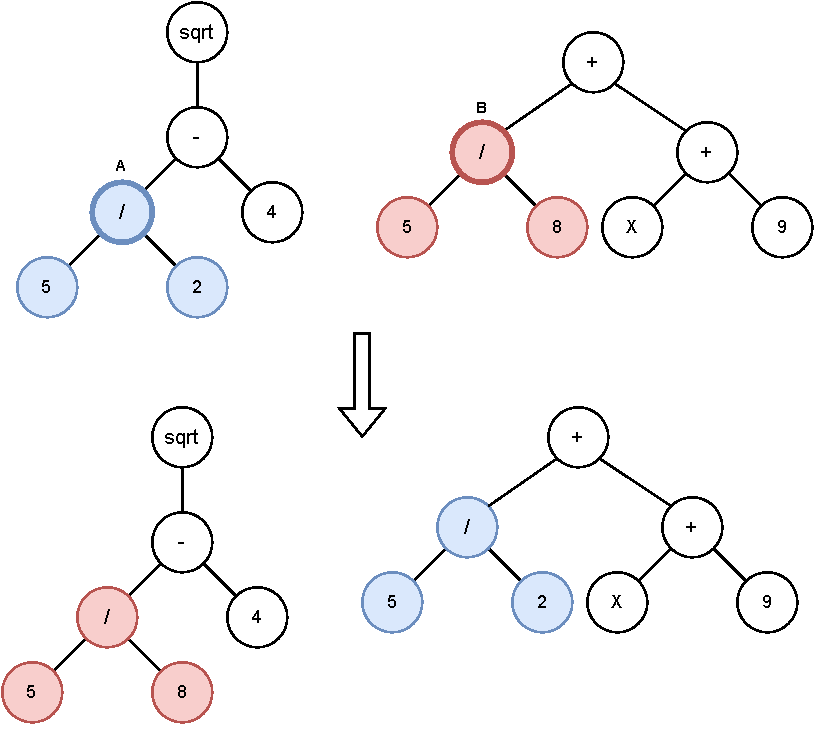
\includegraphics[scale=1]{obrazky-figures/tgp-crossover.pdf}
    \caption{Genetický operátor křížení}
    \label{fig:tgp-crossover}
\end{figure} 
\vspace{0.5cm}

\subsection{Mutace}

Tento unární operátor přináší ve vybraném rodiči náhodné změny a zajišťuje nový genetický materiál, čímž se často předejde konvergenci k~lokálnímu optimu. Nejprve se vybere jeden rodič na němž bude operátor mutace aplikován, následně je náhodně vybrán stromový uzel v~němž k~mutaci dojde. Na zvoleném místě je poté vygenerovaný nový podstrom o~maximální určené výšce. Někdy to může být i pouze jeden uzel, pokud se bod mutace nachází v~maximální hloubce. Občas může dojít k~mutaci již na úrovni kořenového uzlu, čímž se většinou znehodnotí celý program. Mimo variantu generující podstromy existuje varianta, která prochází systematický celý strom a u~každého uzlu dochází s~jistou pravděpodobností k~mutaci, jinak též zvaná bodová mutace. Na obr.~\ref{fig:tgp-mutation} lze vidět variantu generující podstrom v vybraném bodě A. 

\vspace{0.5cm}
\begin{figure}[h!]
    \centering
    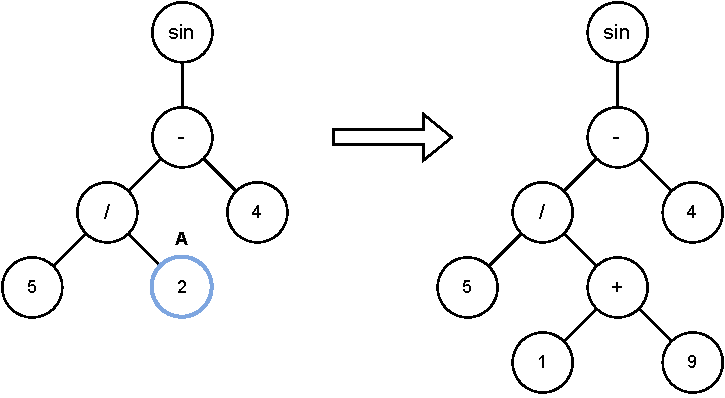
\includegraphics[scale=1]{obrazky-figures/tgp-mutation.pdf}
    \caption{Genetický operátor mutace}
    \label{fig:tgp-mutation}
\end{figure}
\vspace{0.5cm}


\section{Srovnání s dalšími evolučními algoritmy}
Jak již bylo zmíněno na začátku kapitoly, genetické programování je silně inspirováno \textbf{genetickými algoritmy} (GA) a sdílí spolu veliké množství vlastností. Obě techniky využívají podobné genetické operátory, snaží se prohledávat prostor a zároveň neuváznout v~lokálním minimu, negarantují nalezení globálního optimálního řešení, ale snaží se konvergovat k~vhodnému řešení v~rozumném čase. Jeden z~rozdílů je možné zaznamenat v~reprezentaci jednotlivých řešení, viz obr.~\ref{fig:ga_vs_gp}, kde GA reprezentuje populaci jako řetězce čísel neměnné délky, zatímco GP je v~jeho základní reprezentaci tvořeno syntaktickými stromy, které pokud nejsou uživatelem explicitně omezeny, tak můžou dosahovat nekonečných velikostí. Rozdíl je taktéž v~aplikaci genetického operátoru křížení -- v~GA se genetický materiál často vyměňuje na stejných pozicích, zatímco v~GP se vybrané podstromy mění na různých pozicích. Ačkoliv všechny tyto výše zmíněné rysy se dají modifikovat, ta důležitá rozdílnost spočívá v~interpretaci řešení a tedy mapování popisu problému na objekt řešení. To v~GA může být \emph{1 to 1} nebo \emph{many to 1}, u~GP je to vždy \emph{many to 1}~\cite{GAorGP}.

\begin{figure}[!h]
    \centering
    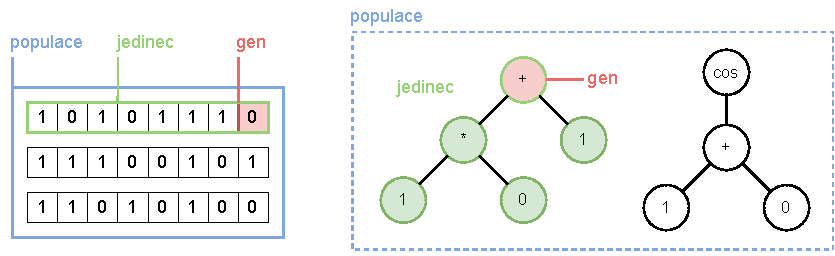
\includegraphics[scale=1]{obrazky-figures/tgp-differences-ea.pdf}
    \caption{Srovnání reprezentace populace, jedince a genu v genetickém algoritmu (vlevo) a genetickém programování (vpravo).}
    \label{fig:ga_vs_gp}
\end{figure}

\textbf{Evoluční strategie} (ES) využívá vektorovou reprezentaci, kde každý prvek vektoru představuje jeden parametr řešení. Mezi genetické operátory se řadí rekombinace a mutace (jakožto hlavní operátor~\cite{EvoFitLectures}), kde nový jedinec vzniká přidáním náhodného čísla ke každé hodnotě rodičovského vektoru. Dokážou pracovat s reprezentací chromozomů ve vícerozměrném prostoru. Jeden z výrazných rysů ES se nazývá pokročilá samoadaptace parametrů, kdy se tyto parametry mění za běhu specifickým způsobem, například samoadaptace velikosti mutačního kroku. Nedávné formy ES se dokonce řadí mezi špičkové algoritmy sloužící k optimalizaci netriviálních funkcí reálných čísel~\cite{eiben-2015B}. 

\textbf{Evoluční programování} (EP) nemá striktní pravidla pro reprezentaci jedinců.  Klasické EP reprezentovalo jedince v~podobě konečných automatů, novodobé pomocí vektorů reálných čísel, takže se velmi přiblížilo ES a lze jej tedy někdy chápat jako speciální případ ES. Hlavní rozdíl, kde se tyto techniky odlišují, spočívá v~biologické inspiraci, kde každý jedinec je považován za odlišný druh, proto zde neexistuje žádný rekombinační operátor a~pouze jediným tu je tedy mutace~\cite{eiben-2015B}. Tím pádem každý jedinec populace generuje pouze jednoho potomka na rozdíl od GP, kde genetické operátory můžou generovat až dva potomky.

\section{Nedostatky stromového GP}
Ačkoliv je stromová technika GP tou nejznámější, tak skýtá i pár problémů. Protože velikost řešení zde není prakticky omezená, tzn. syntaktické stromy reprezentující jednotlivá řešení můžou nabývat jakékoliv výšky, omezení je většinou dáno jen u~generace první populace, tak zde může docházet k~tzv. \emph{bloatu}, což znamená nadměrný růst řešení v~průběhů generací, které je většinou způsobeno genetickými operátory. Neexistuje univerzální řešení a často závisí na implementaci. Řešení tohoto problému jsou navržena v~praktické části této práce. 

Vyhodnocení stromové reprezentace programu je často velmi náročné, obzvláště pokud jsou řešení komplexní nebo dochází k~výše zmiňovanému nekontrolovatelnému růstu. To jak bude řešení komplexní závisí i na výběru neterminálních symbolů, které tvoří vnitřní uzly, a jejich aritě. Stromové uzly často nejsou uloženy v~paměti kontinuálně. Toto může mít za následek pomalejší přístup do pamětí. Taktéž rekurze využívaná ve stromových strukturách je výpočetně náročná operace (zejména u~jazyků jako je C nebo Python, které implementují rekurzi jako volání nové funkce včetně zásobníkových operací), jež si žádá alokaci většího množství paměti~\cite{RecursionAndLooping}. Proto lze v~literatuře~\cite{Brameier1998} často vidět GP implementováno pomocí jazyka LISP, který je považován za funkcionální jazyk, a prefixové notace.   

% ===================================================
% KAPITOLA 3 -- LINEÁRNÍ GENETICKÉ PROGRAMOVÁNÍ

\chapter{Lineární genetické programování}\label{ch:3}
Lineární genetické programování je jedna z dalších variant GP. V~této kapitole je detailně popsána její charakteristika, reprezentace programů, postupy jakými se tyto programy inicializují, genetické operátory včetně grafické ilustrace a na závěr krátké porovnání se stromovou variantou GP. Zdrojem informací pro tuto kapitolu je literatura~\cite{LGP}. Tato technika reprezentuje jednotlivá kandidátní řešení jako sérii instrukcí, jež se vykonávají v~sekvenčním pořadí jako v~tradičním imperativním jazyce nebo jazyce symbolických instrukcí. Nejen že se tato varianta GP vyznačuje kompaktností generovaných řešeních, ale také umožněním velmi malých variačních změn v programech~\cite[str. 8]{LGP}. Je využívána například v~problémech, kde je zapotřebí vykonat určité instrukce ve specifickém pořadí, jako např. kontrolní systémy~\cite{realtimefeedback}, kde se ve zmíněném problému tato metoda projevila jako nejúčinnější.

\section{Reprezentace programu}
Program se skládá ze sekvenčně se vykonávajících instrukcí. Každá instrukce může být složená z~operace a operandů, které mohou být vyjádřeny registrem či konstantou. Na pravé straně se nachází zdrojové operandy a operace a na levé cílový registr pro uložení výsledku. V~inicializační fázi je vždy stanovena množina možných konstant, operací a skupina registrů. Na obrázku~\ref{fig:lgp_rep} lze vidět příklad matematického programu zapsaného v~jazyce C využívající jednoduché aritmetické operace, 7 vstupních registrů a jeden registr výstupní.

\begin{figure}[!h]
    \centering
    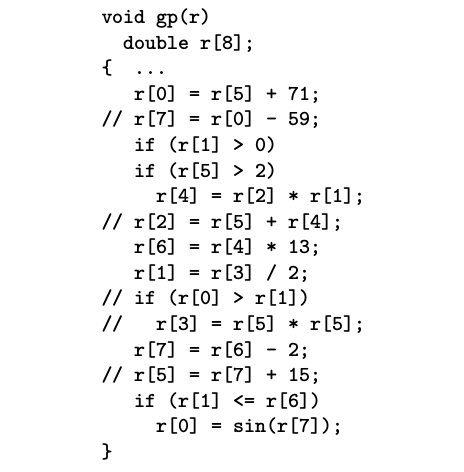
\includegraphics[scale=0.45]{obrazky-figures/lgp-program-in-c.png}
    \caption{Reprezentace lineárního GP v~notaci jazyka C. Převzato z~lit.~\cite[str. 14]{LGP}.}
    \label{fig:lgp_rep}
\end{figure}

Programová řešení nejsou omezena pouze na jednoduché instrukce, ale mohou podporovat i složitější koncepty. Zatímco ve stromovém GP existují různě neterminální uzly s~podmínkou, které zaručují různé chování programu na různé vstupní situace, tak obdobný koncept lze realizovat v~lineárním GP větvením programů, které může být implementováno podmíněnou instrukcí např. \texttt{if (x < 5) then} a následně počtem instrukcí, které se po splnění této podmínky vykonají. Existují zde i vnořené podmínky, kdy je několik podmínek pod sebou spojeno logickými operátory konjunkce (\texttt{AND}) nebo disjunkce (\texttt{OR}). Druhá varianta je podpora podprogramů, kdy se opět po splnění podmínky odkazuje na místo v~paměti označující daný podprogram po jehož ukončení se pokračuje ve vykonávání hlavního programu. Koncepce iteračních bloků kódu není v~lineárním GP zas až tak důležitá a~hlavně častá. Mimo jiné s~sebou přináší řadů problémů, které je potřeba řešit. To zahrnuje možné nekonečné zacyklení nebo třeba vnořené cykly.

\section{Charakteristika lineárního programu}
Jeden z~důvodů vzniku lineárního GP bylo překonat různé nevýhody spjaté s~tradičním stromovým GP, které zahrnují nevhodnou reprezentaci genotypu nebo náročné vyhodnocování. Velmi charakteristické pro tuto sekvenční reprezentaci jsou například nevyužité části programového kódu. S lineárním GP se proto pojí následující pojmy.

Pokud se v~programu nachází taková instrukce, která ovlivňuje výslednou hodnotu programu, nebo fitness hodnotu alespoň pro jeden možný vstup daného problému, tak je nazývána \textbf{efektivní instrukcí}. Naproti tomu \textbf{neefektivní instrukcí} nebo \textbf{intronem} jsou nazývány ty instrukce, které mají nulový vliv na výsledek pro celou množinu různých vstupů. Další možný výklad tohoto termínu by mohl být, že nemá žádný vliv na konečnou hodnotu funkce fitness. Neefektivní instrukce může být z~programu odstraněna, viz obr.~\ref{fig:introns-removal}, nebo zachována. Na obr.~\ref{fig:lgp_rep} je neefektivní instrukce v~rámci programu značená symboly dvou lomítek \texttt{//}, čímž tedy není při interpretaci vykonána, ale je nadále jako genetický materiál zachována.

\textbf{Strukturální intron} označuje v~programu takovou neefektivní instrukci, jež vznikla z~manipulace s~neefektivními registry, které nemají vliv na konečný výsledek programu. Ve stromovém GP k~strukturálním intronům nedochází. Algoritmem který program zpětně analyzuje, tedy každou instrukci a její cílový registr a závislost tohoto registru na předchozí instrukci, lze eliminovat neefektivní kód, který zefektivní následné vyhodnocování fitness funkce. Velký vliv na vznik těchto neefektivních úseků kódu mají třeba parametry délky programu nebo počtu registrů. 

\textbf{Sémantickým intronem} je nazývána ta neefektivní instrukce nebo skupina neefektivních instrukcí, jež jsou strukturálně správně, tedy manipulují s~registry, které mají vliv na výsledek programu, ale zjednodušeně řečeno, hodnota efektivních registrů se po provedení instrukce nijak nezmění. Na vznik těchto intronů má z~největší části vliv vybraná množina instrukcí a konstant. Nelze se jim v~lineárním GP bohužel úplně vyhnout, ale je dobré si stanovit a formulovat pravidla k vyvarování se alespoň těm nejzákladnějším intronům a~zároveň zanechání dostatečného prostoru evoluci.

\newpage
\begin{figure}[!h]
    \centering
    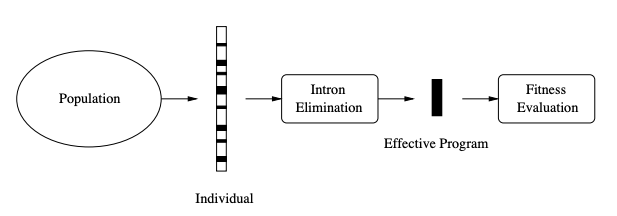
\includegraphics[scale=0.6]{obrazky-figures/lgp-introns.png}
    \caption{Obecný proces odstranění neefektivních instrukcí (vyznačeny bílou barvou). Převzato z~lit.~\cite[str. 39]{LGP}.}
    \label{fig:introns-removal}
\end{figure}

\begin{center}
$(a) \quad r_0 := r_i/0 
  \quad  \quad  \quad (b) \quad r_1 := r_0 - r_0 
\quad \quad r_0 := r_i/r_1 $ \\ 
\vspace{0.6cm}
$ (c) \quad if \, (r_i > r_i) 
\quad \quad r_0 := r_j + c $   \\
\vspace{0.6cm}

Příklady sémantických intronů -- dělení nulou (a), (b) a nenaplnitelná podmínka (c), tudíž nikdy nedojde k~vykonání instrukce, jež je závislá právě na této podmínce.
\end{center}
\vspace{0.3cm}

Detekce a odstranění není sémantických intronů již tak zcela snadné jak tomu bylo u~strukturálních. Programy dosahují dostatečného zrychlení již odstraněním  strukturálních intronů a~je tedy otázkou, zdali se vůbec vyplatí algoritmus pro odstranění těch sémantických intronů implementovat. Možnou motivací by mohla být snadnější interpretace a~porozumění jednotlivým programovým řešením~\cite[str. 44]{LGP}.

\section{Inicializace populace}
 U~varianty lineárního GP existují několik klíčových faktorů, které ovlivňují to, jak bude generovaná populace vypadat. Těmito faktory, parametry, jsou 
 zde délka programu a počet registrů. U~délky programu je třeba stanovit dolní a horní hranici. Oba tyto parametry musí být zvoleny s~rozvahou a úměrou vzhledem k~velikosti problému. Je neefektivní například generovat dlouhé programy o~stovkách řádcích k~vyřešení jednoduchého matematického problému. Nejen že by opakované vyhodnocování tohoto programu zabralo velké množství času, ale zřejmé by nikdy nedošlo k~nalezení nejlepšího řešení.
Zde je uvedeno několik inicializačních technik. 
\begin{itemize}
    \item \textbf{Volná inicializace} -- Zahrnuje standardní inicializaci bez omezení.
    \item \textbf{Plně efektivní inicializace} -- Program nebude obsahovat neefektivní instrukce,  tzv. \emph{introny}.
    \item \textbf{Maximální inicializace} -- Inicializace programů v~jejich maximální možné délce.
    \item \textbf{Konstantní inicializace} -- Inicializace všech programů v~délce určené konstantou.
    \item \textbf{Proměnlivá inicializace} -- Programy budou mít proměnlivou délku na základě definovaného rozsahu.
\end{itemize}

\section{Genetické operátory}
\subsection{Mutace}
Mutační operátor je klasifikován do dvou kategorií -- mikro mutace a makro mutace. Makro mutace manipuluje s instrukcí s jakožto atomickým prvkem, takže operací s ní spojené se dějí na úrovní celých instrukcí. Kdežto mikro mutace se zaměřuje na změnu prvků uvnitř instrukce. Ta může zahrnovat změnu konstant, registrů či operací. U makro mutací se rozlišují následující tři operace (definované zkratky -- $l(gp)$ vyjadřuje délku programu; $l_{min},\;  l_{max}$ minimální a maximální délku programu):
\begin{itemize}
    \item \textbf{Aditivní mutace} -- Před vybranou instrukci je vložena nová instrukce za podmínky, že je splněno $l(gp) < l_{max}$, viz obr.~\ref{fig:lgp-macro-add-mutation}.
    \item \textbf{Destruktivní mutace} -- Vybraná instrukce je odstraněna za podmínky, že $l(gp) > l_{min}$, viz obr.~\ref{fig:lgp-macro-destructive-mutation}. Je doporučeno vzájemně aplikovat s aditivní mutací k předcházení nadměrné redukci programu.
    \item \textbf{Měnící mutace} -- Vybraná instrukce je nahrazena za jinou, viz obr.~\ref{fig:lgp-macro-mutation}, kde dochází k výměně instrukce A za instrukci B.
\end{itemize}

\begin{figure}[!h]
    \centering
    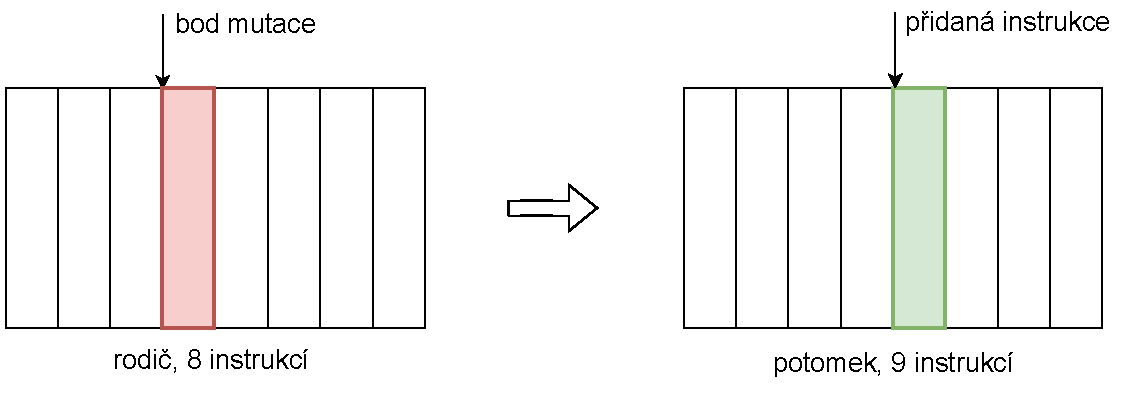
\includegraphics[scale=0.65]{obrazky-figures/lgp-mut-additive.pdf}
    \caption{Aditivní mutace}
    \label{fig:lgp-macro-add-mutation}
\end{figure}

\begin{figure}[!h]
    \centering
    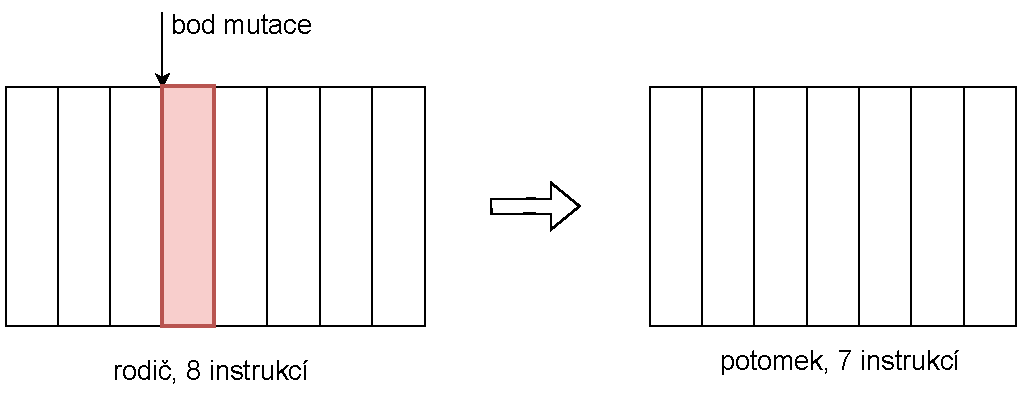
\includegraphics[scale=0.65]{obrazky-figures/lgp-mut-destructive.pdf}
    \caption{Destruktivní mutace}
    \label{fig:lgp-macro-destructive-mutation}
\end{figure}

\begin{figure}[!h]
    \centering
    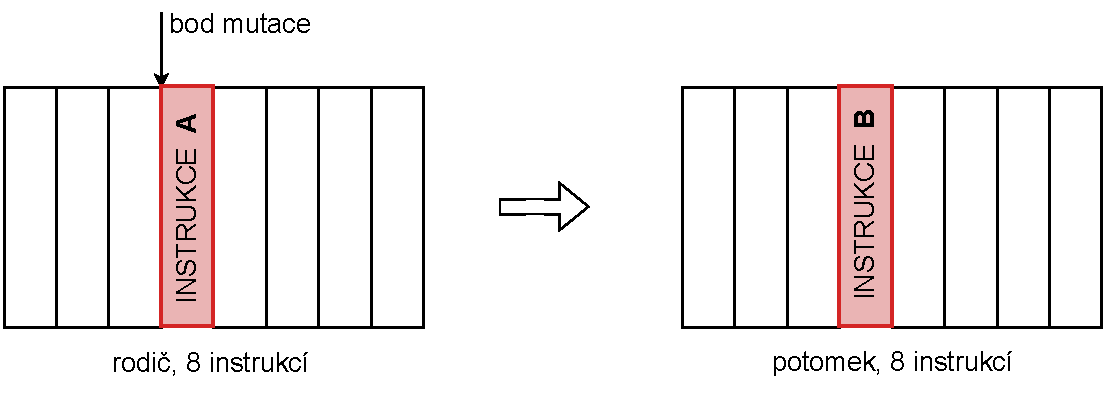
\includegraphics[scale=0.65]{obrazky-figures/lgp-mut-mut.pdf}
    \caption{Měnící mutace}
    \label{fig:lgp-macro-mutation}
\end{figure}


\newpage
\subsection{Křížení}
Křížení je segmentový variační operátor, který vytváří v závislosti na implementaci jednoho či dva nové potomky z dvou vybraných rodičů. Tato metoda spočívá v tom, že chromozomy rodičů se rozdělí na dva či více segmenty a ty  se pak následně mezi sebou vymění. Existují dva základní typy tohoto operátoru.
\begin{itemize}
    \item \textbf{Jednobodové křížení} -- 
    V~obou rodičích je náhodně zvolen jeden bod, ve kterém následně nastane křížení, kdy se vymění poslední segmenty obou rodičů, viz obr.~\ref{fig:lgp-crossover-one-point}. Pokud je jeden z~potomků delší než je maximální délka programu, tak proběhne křížení znovu, ale se zvolením stejné pozice křížení v~obou rodičích. Často zde dochází k větší absolutní velikosti kroku v porovnání s vícebodovým křížením.
    \item \textbf{Vícebodové křížení} -- Jsou zvoleny dva body křížení v~obou rodičích, z nichž druhý je dán délkou segmentu od prvního bodu. Prostřední segmenty obou rodičů, jež se mezi těmito dvěma body nachází, se poté vzájemně vymění, viz obr.~\ref{fig:lgp-crossover-two-point}. 
\end{itemize}

\vspace{0.3cm}

\begin{figure}[!h]
    \centering
    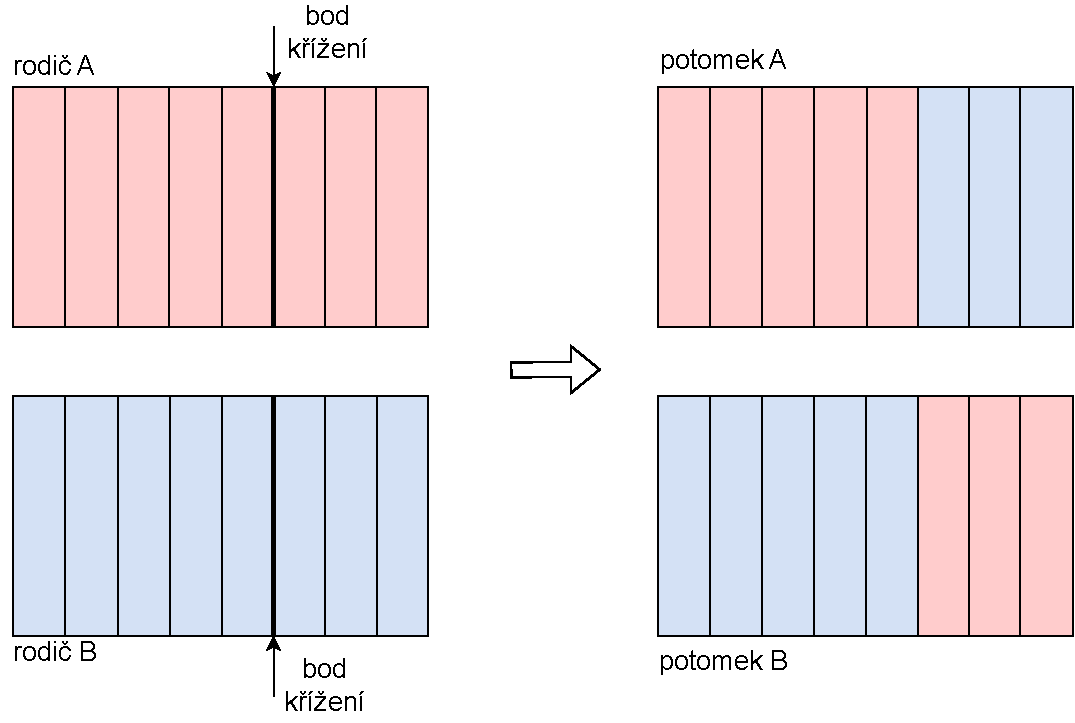
\includegraphics[scale=0.65]{obrazky-figures/lgp-cross-one.pdf}
    \caption{Jednobodové křížení}
    \label{fig:lgp-crossover-one-point}
\end{figure}

\begin{figure}[!h]
    \centering
    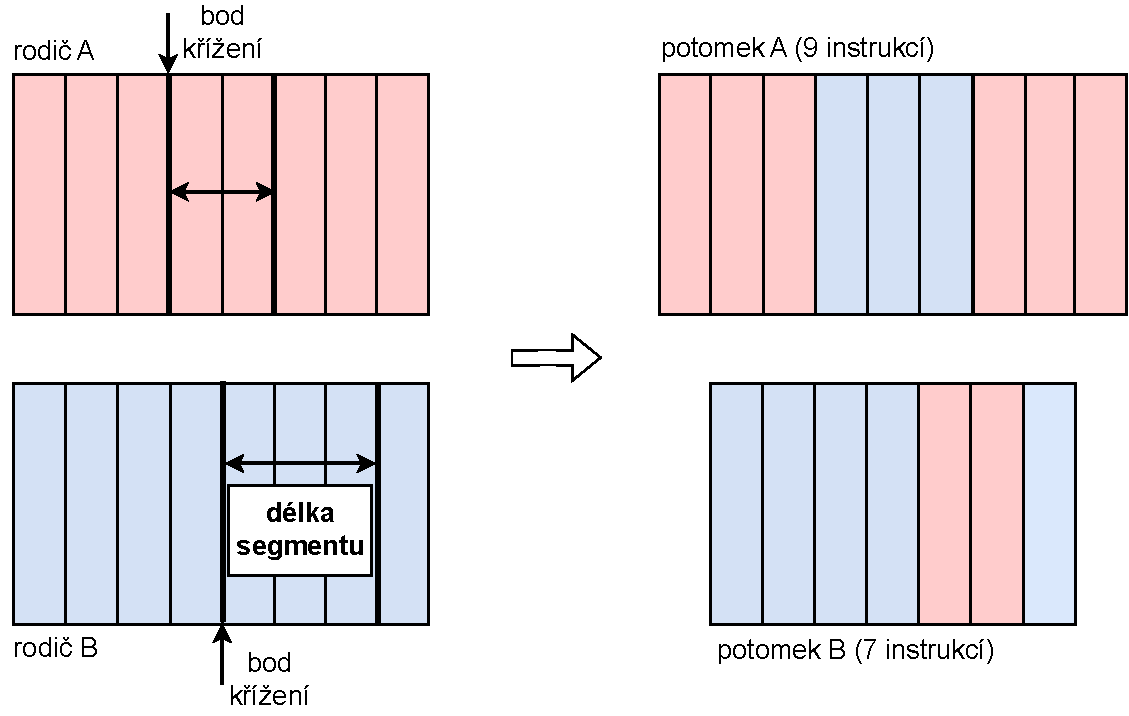
\includegraphics[scale=0.65]{obrazky-figures/lgp-cross-two.pdf}
    \caption{Dvoubodové křížení}
    \label{fig:lgp-crossover-two-point}
\end{figure}

\newpage
\section{Srovnání se stromovým GP}
Stromové a lineární genetické programování jsou techniky GP, které sdílejí podobné koncepty, ale i kvůli na první pohled odlišné programové reprezentací implementují spoustu věcí odlišně a vykazují i jiné chování. Stromové GP implementuje datový tok omezený stromovou strukturou, zatímco lineární GP využívá mnohem flexibilnějšího datového toku v~registrech. Komplexita a náročnost vyhodnocování těchto reprezentací je značně odlišná. U~stromového GP je potřeba rekurzivně procházet stromovou strukturu, zatímco u~lineárního GP jsou sekvenčně zpracovávány instrukce jako u~strojového kódu. Bylo tomu dokázáno na kolekcí dvou benchmarků, jež navzájem tyto dvě techniky porovnávaly~\cite[kap. 8]{LGP}. Taktéž se na základě něj prokázalo, že lineární GP je schopno vytvářet menší a efektivnější programy. Nejen že těží z~výhody právě své reprezentace, která neskýtá mnohá omezení, ale taktéž znovu využívá obsahy registrů a odstraňuje neúčinný kód, zatímco stromové GP vykoná program bez ohledu na efektivitu. Právě i proto je lineární GP flexibilnější strukturovaným změnám oproti syntaktickému stromu ve stromovém GP, kde je velice obtížné přidávat anebo odstraňovat vnitřní uzly. Vložením či odstraněním instrukce u~lineárního GP nejsou ztraceny případné podstruktury programu jak by tomu bylo u~stromového GP. Obě techniky implementují odlišným způsobem i genetické operátory, podrobněji viz předchozí kapitoly. Zatímco u~stromového dochází ke křížení stromových podstruktur v~náhodně vybraném bodu, tak u~lineárního  je možné aplikovat i vícebodové kříženi s~variabilní délkou segmentu. Mutační operátor u~stromového GP běžně generuje v~bodu mutace náhodný podstrom, zatímco u~lineárního je rozlišováno mezi mikro a makro mutacemi.

% ===================================================
% KAPITOLA 4 -- APLIKACE GENETICKEHO PROGRAMOVANI

\chapter{Aplikace a vývoj genetického programování}\label{ch:4}
Genetické programování našlo již mnohé uplatnění v~řešení různých problémů. V~této kapitole jsou krátce zmíněné aplikace GP, jak na ty nejzákladnější úlohy na kterých je často tato technika představována, tak i  složitější. Použití GP má zcela mnoho výhod -- dokáže automaticky generovat programy, které mohou řešit komplexní problémy, které jsou jen stěží řešitelné pomocí konvenčních metod, ať již programování nebo jiných metod strojového učení. Je praktické při problémech, kde není jasné, jakým postupem se dostat k~požadovanému výsledku, dále taktéž pokud je nutné před výpočtem předzpracovat a klasifikovat velký objem vstupních dat~\cite{Koza:2010:GPEM}. Mezi další vlastnosti a benefity použití této techniky patří:
\begin{itemize}
    \setlength\itemsep{0.01em}
    \item podpora veliké škály programových struktur, znovupoužití kódu,
    \item optimalizace a paralelní zpracování,
    \item redukce doby vývoje,
    \item prohledávaní širokého prostoru možných řešení,
    \item nezávislost na řešeném problému,
    \item přínos konkurenceschopných výsledků.
\end{itemize}
\noindent Obzvláště poslední bod připomíná důležitost toho, proč je GP tak stále využívané. Aby produkovalo užitečné výsledky, namísto pouze řešení problémů, které se ve vědeckých disciplínách nazývají \emph{toy problem}, které tedy nejsou pro vědu nikterak užitečné a slouží spíše pro demonstrační ukázky nějaké obecné techniky~\cite{gptrends}. Pokud není jinak konkrétněji uvedeno, vychází tato kapitola z~literatury~\cite{Brameier1998, Koza:2010:GPEM}.

\section{Aplikace genetického programovaní}
\begin{itemize}
    \item \textbf{Symbolická regrese} -- Jeden z~nejznámějších problémů na kterém je GP prvotně demonstrováno, je právě symbolická regrese. Cílem programu je nalézt takovou matematickou rovnici, která splňuje podmínky pro zadané vstupní a výstupní hodnoty a tedy najít souvislost mezi těmito daty. Na počátku je vygenerována populace programů, kde jsou funkční symboly reprezentovány matematickými funkcemi (např. +, -, *, /, sin, cos, \dots) a terminály proměnnými či konstantami. Fitness funkce následně měří přesnost každého kandidátního řešení na daném datasetu. Ta je měřena na základě odchylky mezi očekávanými a aktuálními výsledky. Tento problém může být aplikován na širokou řadu aplikací včetně funkčních aproximací, identifikaci systému nebo vhodnosti nějakého modelu. Je aplikován v~různých oborech, např. v~inženýrství, biologii či financích.

    \item \textbf{Analogové obvody} --  Zatímco jednoduché obvody lze řešit pomocí tradičních výpočetních metod, u~složitějších problémů, jako je třeba návrh komplexní ALU jednotky, se tento proces stává časově náročným. Jednotlivé programy jsou stromově reprezentovány obsahující logické členy (AND, OR, NOT), sčítačky (celá, poloviční, \dots) a klopné obvody (JK, RS, D, \dots). Terminálními symboly jsou reprezentovány proměnné uvnitř obvodu. Kalkulace fitness hodnoty zde probíhá na základě pravdivostní tabulky, která nastiňuje vztahy mezi vstupy a výstupy obvodu. Pokud je dosáhnuto požadované hodnoty fitness, tak je provedena validace elektrického obvodu, zdali je plně vyhovující~\cite{analog_digital_circuits}.
    
    \item \textbf{Cart centering problem} -- V~tomto problému se snaží GP nalézt takovou řídicí strategii, která vyvine dostatečnou sílu k~posunutí vozíku na přímce na předem určené místo za co nejlepší čas. Tento problém zahrnuje systém, jehož stav je popsán stavovými proměnnými. To znamená aktuální pozici $x(t)$ a rychlost $v(t)$. Nachází se zde taktéž jedna kontrolní proměnná tzv. \emph{big-bang} síla, která dokáže posunout vozíkem jak v~pozitivním tak negativním směru. Její hodnotu se snaží program určit tak, aby se systém dostal do cílového stavu za co nejlepších podmínek. Ty můžou být měřeny například v~ceně nebo času~\cite{Brameier1998}.
\end{itemize}

Genetické programování se už běžně používá jako metoda řešení různých problémů v~mnoha oblastech včetně hydrologie, hydrauliky, prediktivního modelování, elektronice, klasifikace obrázků, diagnostiky nemocí a mnoha dalších. V~následujících podkapitolách je podrobněji popsáno pár z~nich, např. jak tato metoda dokáže opravovat a vylepšovat software a jak může být užitečná v~inženýrství při návrhu stavebních základů.

\subsection*{Geneticky vylepšený software}
Genetické programování se již osvědčilo v~mnoha případech jako vhodný nástroj k~úpravě či generaci programového kódu~\cite{ApplicationOfGP}. První aplikace a případ užití bylo pro hashovaní, caching a garbage collector, kde i velká moderní paměť a její správa může znamenat značnou režii. Další příklady využití jsou například internetové mashupy, což v~překladu znamená nějakou internetovou stránku, která v~rámci poskytování služeb kombinuje data či funkcionalitu z~více zbrojů, nebo také pro generaci kódu. Kompilátory by totiž neměly pouze vytvářet korektní kód, ale zároveň ideálně krátký a dostatečně efektivní. 

GP se taktéž osvědčilo v~automatické opravě programového kódu. Ačkoliv se podle několika teoretických analýz a studií stále jedná o~ne velmi rozšířenou metodu. Na mnoha příkladech se snaží GP využít již napsaný kód, který se snaží přeskupit. A~zde to platí ještě víc, že jeden řádek kódu může rozbít celý program, ale taktéž můžou v~rámci mutace nebo křížení vzniknout kvalitní programy. Tato technika dokázala vyřešit problém nalezený 31.~prosince 2008, kdy uživatelé zaznamenali rozsáhlý bug v~přehrávačích Microsoft Zune, který zapříčinil jejich zamrznutí. Tento příklad vychází z~článku~\cite{AutomaticBugFixing}.

\subsection*{Aplikace GP v~inženýrských systémech}
V~posledních letech bylo dokázáno, že GP je úspěšné i v~oblasti návrhu geotechnických systémů~\cite{ApplicationOfGP}. Materiály které se s~tímto inženýrstvím často pojí, např. zemina anebo kamení, vykazují ze své podstaty nejisté chování spojené často s~fyzikálními procesy spojené s~tvorbou těchto materiálů. Modelování chování těchto materiálů je často za hranicemi tradičních metod. Proto se nabízela možnost využití umělé inteligence v~této oblasti. Tyto techniky se používají ve strojírenství k~řešení problémů učením se z~příkladů datových vstupů a výstupů. To pomáhá zachytit funkční vztahy mezi daty, i~když základní vztahy jsou neznámé nebo obtížně vysvětlitelné. Podobný koncept je de facto vysvětlen na příkladu symbolické regrese v~podkapitole 4.1. Z~technik umělé inteligence se v~této oblasti velmi dobře uchytila metoda umělých neuronových sítí, ačkoliv se v~poslední době velmi dobře osvědčila právě i~metoda GP. Přestože neuronové sítě byly úspěšné v~analýze a simulaci mnoha aplikací geotechnického inženýrství, tak jsou kritizovány za to, že jsou \uv{černými skříňkami} kvůli jejich nedostatečné transparentnosti a extrakci znalostí. Nejnovější metodou GP, která je pro toto inženýrství používána, se nazývá evoluční polynomiální regrese (EPR). Je to metoda, která využívá polynomiální funkce a genetické operátory k~vývoji matematických výrazů pro regresní analýzu. Z~pohledu transparentnosti jsou klasifikovány jako \uv{šedé skřínky}, u~nichž jsou známy matematické výrazy, které nejsou těžké na interpretaci. Takže tedy o~třídu lepší než neuronové sítě. Ideální by byly samozřejmě \uv{bílé skříňky} u~nichž jsou používány prvotní principy, tedy fyzikální zákony a fungování systému tedy může být jasně vysvětleno.

Jedna z~konkrétních aplikací v~tomto oboru byla provedena při návrhu mělkých základů na nesoudržné půdě. Usazení takovýchto základů je stále velké téma, které je komplexní a~stále ještě ne zcela pochopené. Tento fakt podnítil řadu vědců k~použití GP, konkrétně výše zmíněné EPR techniky, kdy na základě datasetu dokázali model, jenž dosahoval vynikajících výsledků. Na základě pěti vstupních proměnných, jako je například výška a šířka základu nebo hloubka ukotvení základů, generoval výsledné usazení základů. Výsledky tedy prokázaly, že tento model dosahoval nejen eminentních výsledků, ale byl taktéž úspěšnější než tradiční metody a dokonce než umělé neuronové sítě. \\

\section{Aktuální vývoj v oblasti GP}
Výzkum v oblasti GP se nezaměřuje pouze na zkoumání nových aplikací, ale taktéž na poznávání vlastností GP jako samotného, jež ještě nejsou známé. Jedna z~nich je populační diverzita. Diverzita v~populaci je jedna z~klíčových vlastností potřebná k~tvorbě nové populace, jež pomáhá efektivněji nalézt optimálnější řešení. Se ztrátou diverzity v~populaci je riskována rychlá konvergence k~sub-optimálnímu řešení. Zápis z~poslední konference o~GP~z~r.~2022~\cite{GPTPXVIII} se snaží o~tomto problému diskutovat a dokázat, že jisté metriky  dokážou předpovědět důležité informace a pomoci k~dosáhnutí optimálního řešení. 

Existuje celá řada technik, která se o~tento problém zhroucení populace zajímá, ale stále není dostatečně porozuměno, co ji způsobuje, či k~ní přispívá. Diverzita je standardně v~populaci vymezena počtem unikátnosti jednotlivých řešení dle stanovených metrik. Ale tyto metriky jsou jen malým vzorkem, které jsou dnes využívány. Jedna z~nich, která ještě nebyla dostatečně prozkoumána se nazývá fylogenetická, jež určuje diverzitu na základě předků v~populaci. Na obr.~\ref{fig:pop_diverisities} lze vidět dvě rozdílné diverzity. Šipkami jsou zde znázorněny vztahy mezi rodičem a potomky. Listové uzly zde představují aktuální populaci, kde každý jedinec je unikátní. Zatímco na obrázku (a) je zřejmé, že fenotypová rozmanitost je velká (5), tak fylogenetická malá (\emph{mean pairwise distance}\footnote{Mean pairwise distance vyjadřuje vzdálenost vyjádřenou v~počtu hran (v~grafu) v~nejkratší cestě mezi každou dvojici jedinců v~aktuální populaci.} = 2), u~obrázku (b) je tomu zcela obráceně.

\begin{figure}[!h]
    \centering
    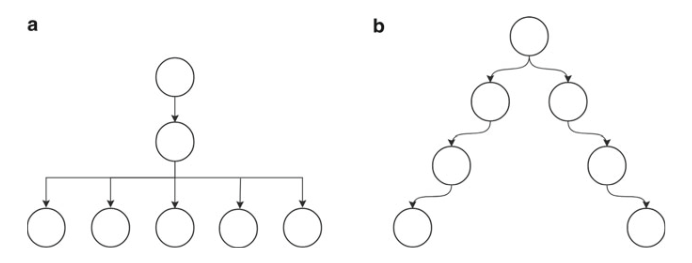
\includegraphics[scale=0.4]{obrazky-figures/diversities.png}
    \caption{Zobrazení dvou různých typů diverzit. Převzato z lit.~\cite[str. 65]{GPTPXVIII}.}
    \label{fig:pop_diverisities}
\end{figure}


Předběžná data podporují dvě hypotézy, že fylogenetická diverzita zachytává data, jež jinší diverzity nezachytávají a zároveň, že může být lepším prediktorem pro úspěch ostatních metrik. Tato studie se snaží za pomocí vybraných selekčních metod a problémů tyto hypotézy ověřit.

\begin{figure}[!h]
    \centering
    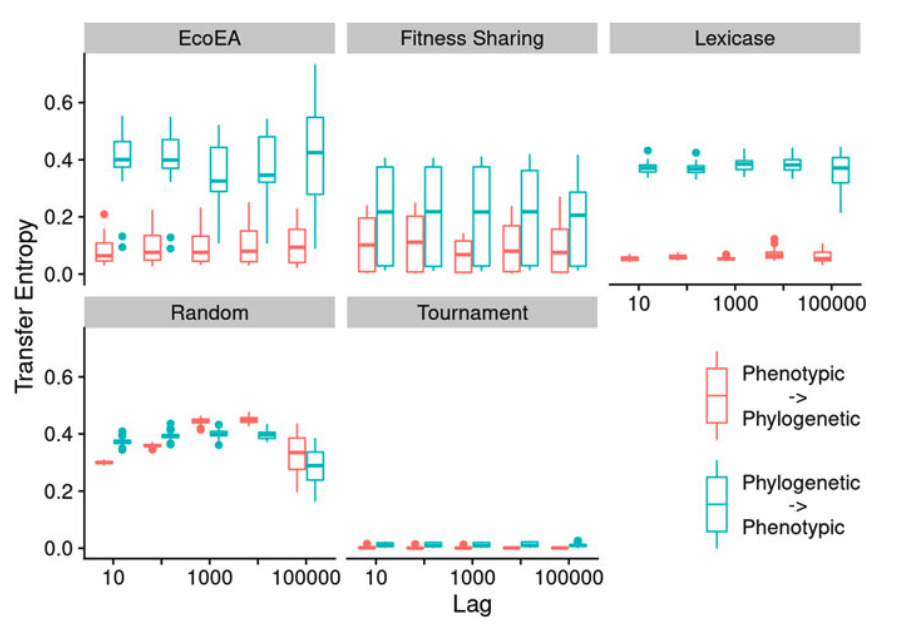
\includegraphics[scale=0.4]{obrazky-figures/diversities-entropies.png}
    \caption{Graf zobrazující míru přenosové entropie ve dvou směrech na různých selekčních metodách a zpoždění. Převzato z lit.~\cite[str. 77]{GPTPXVIII}.}
    \label{fig:diversities-entropies}
\end{figure}


% Jake nove informace se zjistili o fylogeneticke metrice -- cca 5 radku
Na počátku bylo porovnáno několik metrik od obou diverzit. Protože se vyskytla vysoká korelace mezi vybranými metrikami u~fenotypové diverzity, tak byla pro další účely zvolena pouze jedna. U~fylogenetické diverzity byla vybrána střední vzdálenost mezi všemi jedinci aneb \emph{mean pairwise distance}. Ačkoliv při následném porovnávaní výše dvou vybraných metrik byla očekávána vysoká korelace, vzešlo najevo, že je tomu opak a došlo se k~závěru, že se v~průběhu času chovají velmi odlišeně. 

Schopnost předpovídat jedna diverzita druhou byla otestována za pomocí změření přenosové entropie z~fylogenetické diverzity na fenotypovou. Jak lze  vidět na obr.~\ref{fig:diversities-entropies}, tak značně vyšší hodnoty byly nalezeny u~přenosu z~fylogenetické na fenotypovou, což tedy znamená, že fylogenetická diverzita může poskytovat i jiné informace, které ostatní diverzity nemůžou. Menší rozdíly lze pozorovat u~turnajové a náhodné metody, kde se obě diverzity predikují navzájem. Dále byla provedena další analýza za účelem zjištění, zdali výsledky získané na obr.~\ref{fig:diversities-entropies} jsou nějak užitečné, ze kterých následně vyplynulo, že je fylogenetická diverzita skutečně prediktivnější.

Na závěr lze tedy konstatovat, že fylogenetická diverzita obecně více předpovídá úspěch než fenotypová. Stále zde ale záleží na řešeném problému a aplikované selekční metodě. 

% ===================================================
% KAPITOLA 5 -- LANGTONŮV MRAVENEC

\chapter{Úloha Langtonova mravence}\label{ch:5}

Cílem této kapitoly je popsat úlohu Langtonova mravence, na jejíž instancích jsou aplikovány obě dvě varianty GP. Hlavním zdrojem k~této kapitole je literatura~\cite{Brameier1998}. Tato úloha byla poprvé představena Jeffersonem a kol. s~využitím genetických algoritmů. Jejich cílem bylo studium několika základních aspektů genetických algoritmů, kde využili reprezentaci konečných automatů. Později byl tento problém zpopularizován J.~Kozou, jehož přístup k~řešení navrhoval aplikaci GP.   

\section{Princip úlohy}
Tato úloha zahrnuje nalezení kontrolní strategie umělého mravence pohybujícího se ve dvojdimenzionálním poli buněk, jež může obsahovat potravu. Cílem je sesbírat v~co nejlepším čase, tím je zde rozuměno v co nejmenším počtu kroků mravence, všechnu potravu za pomocí sady pravidel sloužících k~navigaci a pohybu mravence. Tato pravidla jsou zakódována v~genu chromozomu jednotlivých kandidátních řešeních. 

\begin{figure}[!h]
    \centering
    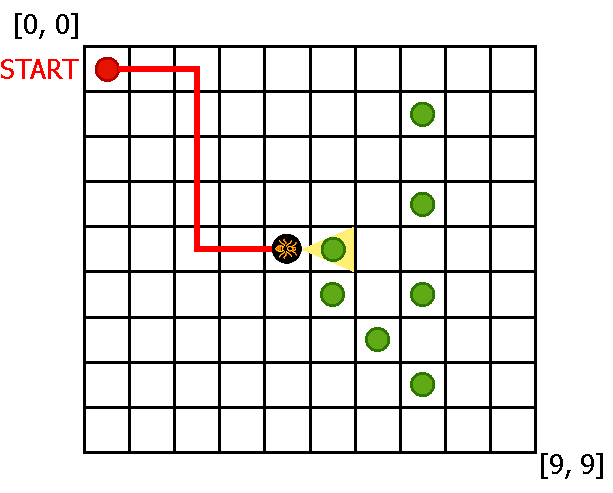
\includegraphics[scale=0.7]{obrazky-figures/langtonsant.pdf}
    \caption{Langtonův mravenec}
    \label{fig:langtons_ant}
\end{figure}

Na obr.~\ref{fig:langtons_ant} lze vidět mřížku o~velikosti 10x10, kde zelená kolečka reprezentují buňky s~potravou, které musí mravenec sesbírat a červená čára znázorňuje jeho dosavadní cestu včetně startovní pozice. Mravenec obvykle začíná na pozici [0, 0], tzn. v~levém horním rohu. Mravenec má v~základu velmi omezené schopnosti pohybu, vidí pouze o~jedno políčko vpřed (na obr. znázorněno žlutým trojúhelníkem) a nemá žádné informace o~své současné pozici.
Literatura aktuálně přistupuje k~tomuto problému pomocí stromového GP a definuje následující sadu pravidel, pomocí níž se může mravenec pohybovat. Protože se jedná o~stromové GP, tak se pravidla dělí na terminální, tedy ty co jsou umístěny v~listech syntaktických stromů a definují pohyb mravence, tak neterminální, tedy funkce pomocí kterých se rozhoduje, jakým způsobem se budou pravidla vykonávat. 
V~aktuálním řešení dle literatury je definována tato sada pravidel.
\begin{description}
    \item \texttt{LEFT} -- Mravenec se na místě otočí o~90° v~protisměru hodinových ručiček.
    \item \texttt{RIGHT} -- Mravenec se na místě otočí o~90° ve směru hodinových ručiček.
    \item \texttt{MOVE} -- Mravenec provede pohyb o~jedno políčko vpřed.
    \item \texttt{PROGN2} -- Binární funkční symbol pro jehož splnění musí být vykonán pravý i levý podstrom.
    \item \texttt{PROGN3} -- Ternární funkční symbol pro jehož splnění musí být vykonán levý, střední a~pravý podstrom.
    \item \texttt{IF-FOOD-AHEAD} -- Podmíněný binární funkční symbol, pokud je podmínka splněna, tak je vykonán levý podstrom, v~opačném případě podstrom pravý.
\end{description}

\vspace{0.2cm}
\begin{figure}[!h]
    \centering
    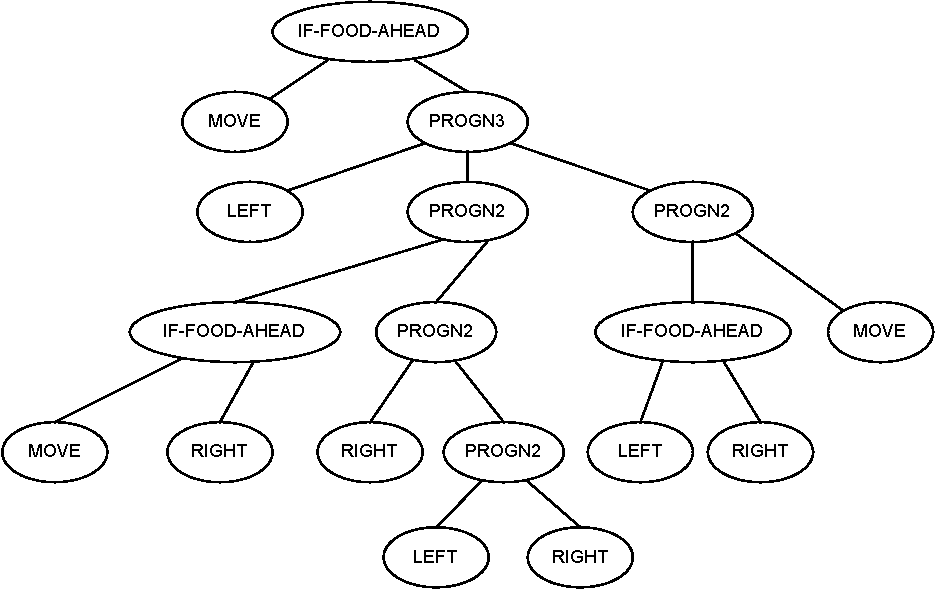
\includegraphics[scale=0.7]{obrazky-figures/lit-santafe-example-tree.pdf}
    \caption{Reprezentace kandidátního řešení úlohy Langtonova mravence. Převzato z~lit.~\cite[str. 154]{Brameier1998} a~graficky upraveno.}
    \label{fig:langtons_ant_tree_rep}
\end{figure}
\vspace{0.2cm}

Na obr.~\ref{fig:langtons_ant_tree_rep} je vyzobrazeno jedno z~nekonečno možných řešení. Při interpretaci tohoto řešení se nejprve mravenec podívá, jestli před sebou vidí potravu, protože kořenový uzel obsahuje funkční symbol \texttt{IF-FOOD-AHEAD}. Pokud potravu vidí, tak se vydá levým podstromem k~instrukci \texttt{MOVE}. V~opačném případě dojde k~vykonání pravého podstromu a funkčního symbolu \texttt{PROGN3}, pro jehož splnění musí být vykonány všechny ostatní podstromy, takže se nejdříve vykoná levý, prostřední a nakonec pravý. Takto analogicky se pokračuje, dokud se nevykoná celý strom.

Úloha je často prezentována na stezkách\footnote{Stezkou je zde myšlena dvojdimenzionální mřížka obsahující políčka s~potravou.}, jež byly navrhnuty jak samotným autorem, tak i osobami, které se o~tento problém zajímaly. Původně byla pro tento problém využívána stezka Johna Muira.

\begin{itemize}
    \item Stezka \textbf{Santa Fe} -- Často používána v~odkazované literatuře, navržena Christopherem Langtonem, viz obr.~\ref{fig:santa-fe}. Je složitější než původní stezka J. Muira.
    \item Stezka \textbf{J. Muira} -- Původně využívána stezka pro tento problém, obsahuje 89 buněk s~potravou, 20 zatáček, 4 mezery, 7 dvojtých mezer a 7 trojtých mezer. 
    \item Stezka \textbf{Los Altos Hills} -- Složitější stezka o~rozloze 100x100 buněk. Pro řešení je ideální přidat nový funkční symbol \texttt{PROGN4}, což je kvartální funkční symbol fungující analogicky jako \texttt{PROGN2/3}. 
\end{itemize}

\begin{figure}[!h]
    \centering
    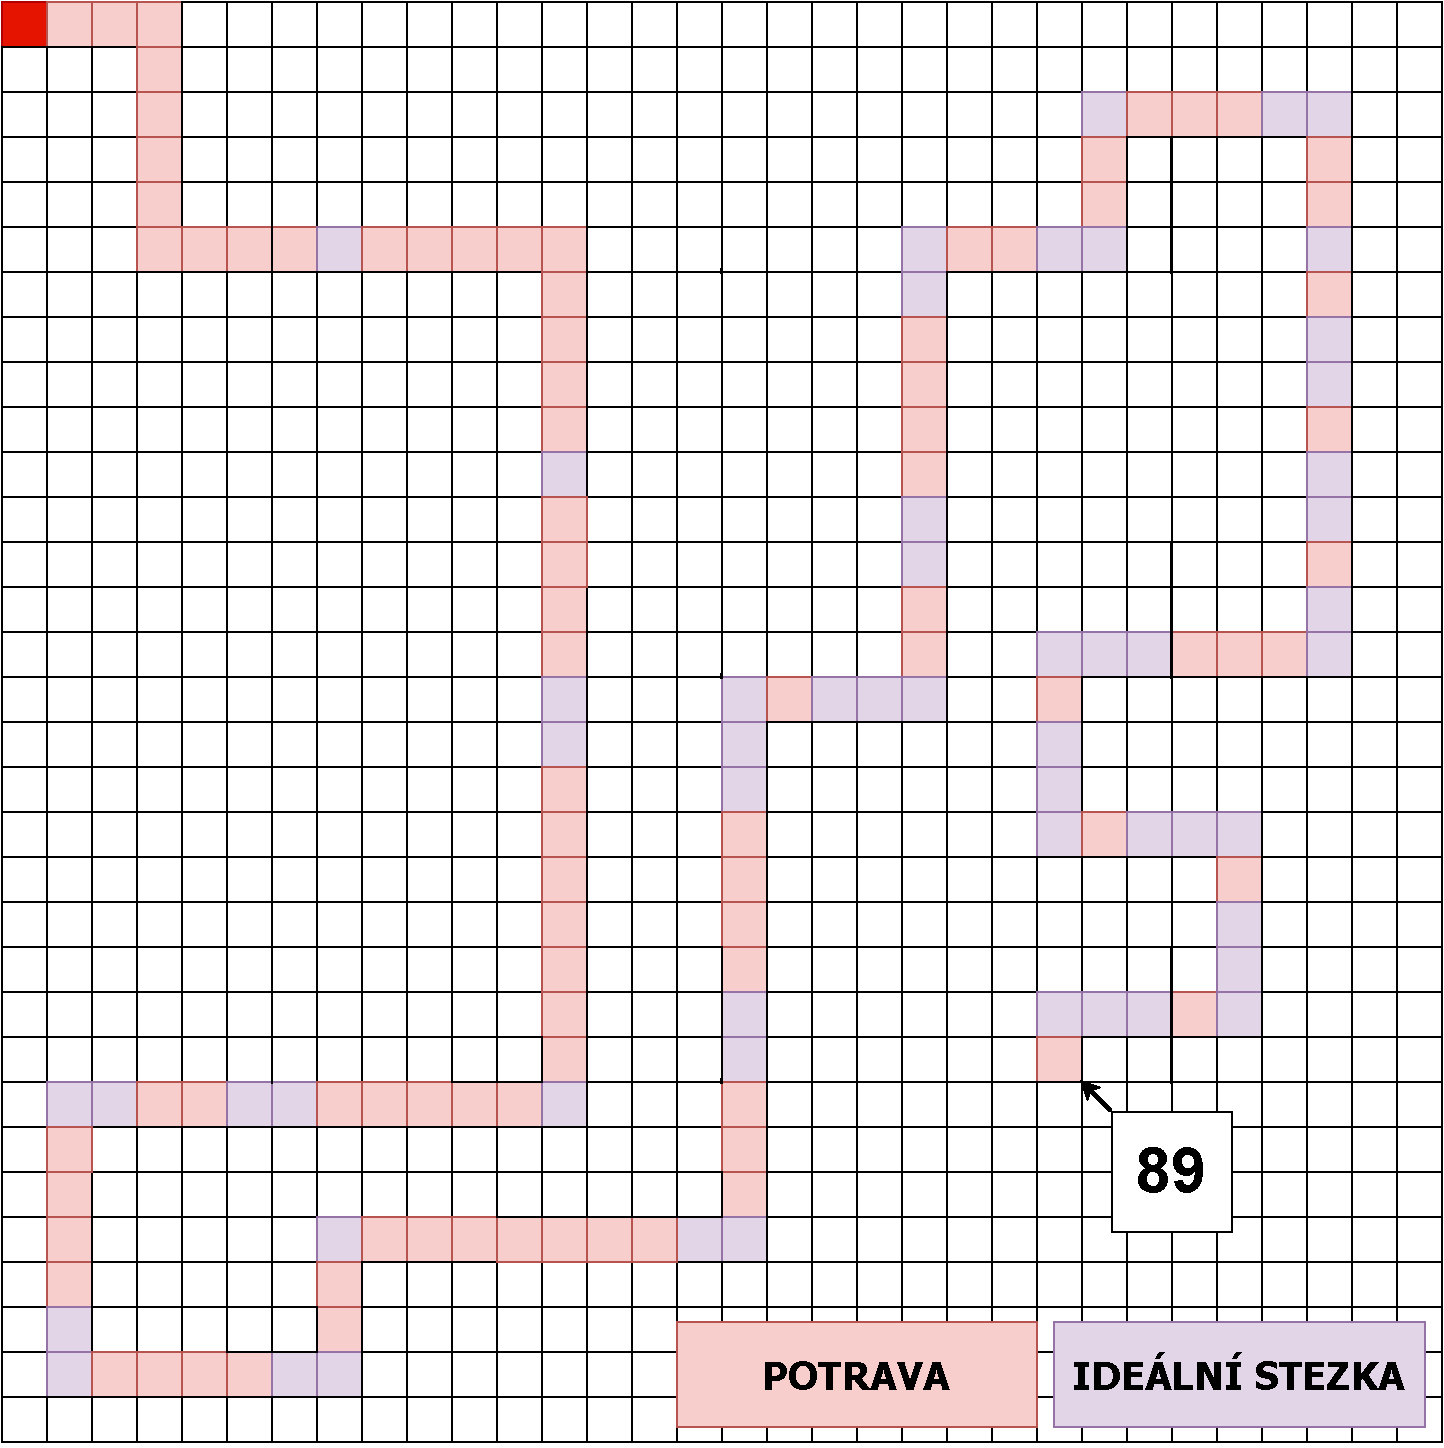
\includegraphics[scale=0.35]{obrazky-figures/santafe.pdf}
    \caption{Stezka Santa Fe (výrazněji červené políčko znázorňuje startovní pozici, číslo 89 v pravém dolním rohu znázorňuje poslední buňku s potravou. Převzato z lit. \cite[str. 55]{Brameier1998} a graficky upraveno.}
    \label{fig:santa-fe}
\end{figure}


\section{Vlastní přístup k~řešení}
K~problému přistupuji velmi obdobně, tak jak je tomu popsáno v~literatuře, která mi byla předlohou. S~odlišnostmi se stavím ke genetickým operátorům či inicializačním parametrům mravence včetně počáteční polohy, která se nemusí vždy nacházet v~levém horním rohu. Rozložení potravy po mřížce je generováno stochasticky, nebo již na předem nadefinovaných stezkách. Ačkoliv je lineární GP v~základu velice tomu stromovému podobné, tak je zde jiná reprezentace programů. Protože mi implementace této úlohy v~této technice nebyla dříve známa, tak jsem se inspiroval stromovým GP a patřičně jsem jej pro tuto techniku upravil. Například jsem musel opustit od funkcí typu \texttt{PROGN2/3}, které jsou zcela typické pouze pro stromové GP a v~lineárním GP nejsou využitelné. Podrobnější implementace je popsána v~následující kapitole.


\chapter{Implementace}\label{ch:6}
V~této kapitole je představen a popsán způsob implementace úlohy Langtonova mravence v~obou variantách GP. Nemalou část implementace tyto varianty navzájem sdílí. Odlišují se hlavně v~návrhu, jak budou jednotlivá programová řešení realizována, následně interpretována a~taktéž jak s~nimi bude zacházeno například při aplikaci genetických operátorů. Ke konci této kapitole je přestaven způsob, kterým je úloha vizualizována uživateli.\\

Pro implementaci byl zvolen jazyk Python3\footnote{https://www.python.org/} a to z~několika důvodů. Poskytuje veliké množství knihoven, které byly k~vývoji použity. Je to multiplatformní jazyk~\cite{payne_2022}, takže je velice snadné tento program spouštět v~různých operačních systémech a distribucích bez větších potíží. Mezi primárně využívané knihovny patří matplotlib\footnote{https://matplotlib.org/}, realizující grafovou vizualizaci, numpy\footnote{https://numpy.org/} pro výpočty nejen u statistického vyhodnocovaní a imageio\footnote{https://pypi.org/project/imageio/} pro výstupní vizualizaci úlohy ve formátu \emph{gif}.

Nejprve jsou shrnuty implementační detaily, jež obě varianty sdílí. Mřížka s~potravou a prázdnými políčky je reprezentována pomocí dvojrozměrné matice obsahující tři různé hodnoty. Nula (0) představuje prázdná políčka, jednička (1) políčka s~potravou a dvojka (2) dosud nalezenou cestu mravencem. Při každém vyhodnocování fitness je tedy počítán počet políček s~hodnotou 1, v~nejideálnějším případě je požadováno, aby se jejich počet rovnal nule, v~tom případě je nalezeno nejlepší řešení. Proto také byla zvolena standardizovaná fitness, která tomuto problému nejlépe vyhovuje. Pro statistické účely jsou v průběhu běhu sbírány hodnoty nejhorší, průměrné a nejlepší této fitness funkce. Obě dvě techniky sdílí stejné implementace selekčních operátorů -- turnaj, ruletu a ranking. 

V~čem se tyto dvě implementace liší, a to zejména v množině symbolů, interpretaci programu a způsob implementace variačních operátorů, je popsáno v~následujících podkapitolách. 

\section{Stromové GP}
Varianta tohoto GP je postavena na základech již existujícího algoritmu sloužícího k výpočtu symbolické regrese~\cite{Sipper2019tinyGP}, jež byla následně upravena, aby vyhovovala problému Langtonova mravence. V~této variantě reprezentují populaci kolekce jedinců, v nichž každý jedinec představuje stromovou strukturu, viz obr.~\ref{fig:langtons_ant_tree_rep}, kde si každý uzel uchovává hodnotu genu, ukazatele na další následovníky a~informace o aktuální pozici a směru mravence včetně jeho aktuálně uražené cesty. Program využívá v~základu množiny terminálních (T) a funkčních (F) symbolů. Jejich význam a funkčnost je popsána v~kapitole~\ref{ch:5}.  


\begin{center}
    \texttt{T = \{ LEFT, RIGHT, MOVE \}} \\
    \texttt{F = \{ PROGN2, PROGN3, IF\_FOOD\_AHEAD \}} \\[0.1cm]
    {\small Množiny terminálních (T) a funkčních (F) symbolů u stromového GP bez rozšíření.}
\end{center}
\vspace{0.3cm}

\noindent Každý tento jedinec tedy představuje instanci stromové třídy, jež obsahuje různé metody mezi které patří například zjištění výšky či velkosti stromu, vygenerování náhodného podstromu ve zvoleném bodě, aplikaci genetických operátorů a další. Interpretace takového jedince probíhá vždy vyhodnocením aktuálního uzlu a pokud je to možné, tak následně vyhodnocením levého podstromu (jinak středního, popřípadě pravého). Tento postup je shodný s metodou procházení stromu \emph{pre-order}. Před vykonáním instrukce \texttt{MOVE} je vždy zkontrolováno, aby se mravenec nedostal za hranice mřížky. Pokud instrukci nelze provést, tak se pozice mravence nemění.

V~rámci řešení operátoru křížení bylo implementováno několik variant, z~nichž se každá vypořádává jiným způsobem s~problémem \emph{bloatu}. V~základu ale tyto varianty fungují téměř podobně, kdy náhodně ze dvou vybraných rodičů vznikne pouze jeden potomek, který je použit pro novou generaci. První varianta křížení se s~problémem \emph{bloatu} vypořádává tím nejjednodušším způsobem. Po vytvoření potomka je provedena kontrola, zdali nový strom vyhovuje maximálnímu výškovému omezení a v~případě nevyhovění je strom zarovnán terminálními symboly. Druhá varianta operátoru postupuje obdobným způsobem, ale namísto zarovnání stromu se provede křížení s~původními rodiči znovu a pokud opět nevyhovuje výšce, tak je s~původními rodiči provedena mutace a případně i poté strom zarovnán.
Mutační operátor je implementovaný ve variantě generující podstromy se standardně omezenou výškou 2 v~náhodně vybraném uzlu mutace. Pokud opět následně potomek nevyhovuje výškovým omezením, tak je zarovnán na maximální hloubku terminálními symboly.

\section{Lineární GP}
Populaci zde tvoří kolekce objektů, jež reprezentují jednotlivá kandidátní řešení, která si udržují svou hodnotu fitness a podrobné informace o~aktuálním řešení problému. Každé kandidátní řešení je definováno kolekcí objektů, instrukcemi, které obsahují informace o~jejím typu a obsahujících datech. Každý jedinec obsahuje několik metod, např. pro výpočet fitness, vložení zjištění délky celého programu, hlavního programu či získání první instrukce požadovaného podprogramu. Reprezentace programu je lineární, kde se jednotlivé instrukce vykonávají sekvenčně. Pro základní variantu této techniky jsou definovány následující množiny terminálních (T) a funkčních (F) symbolů. 

\vspace{0.3cm}
\begin{center}
    \texttt{T = \{ LEFT, RIGHT, MOVE \}} \\
    \texttt{F = \{ IF\_FOOD\_AHEAD ? X : Y \}}\\[0.1cm]
    {\small Množiny terminálních (T) a funkčních (F) symbolů u lineárního GP bez rozšíření.}
\end{center}
\vspace{0.3cm}

\noindent Mimo to program může obsahovat předem definovaný počet podprogramů, které jsou na jejich počátku značeny pomocí návěští ve tvaru \texttt{* SR [X]}, kde \texttt{X} je písmenné označení podprogramu. Na podprogram se odkazuje v~rámci ternárních operátorů. Význam terminálních symbolů je vysvětlen v~kapitole~\ref{ch:5}. Jediný zde přítomný funkční symbol vyjadřuje známý ternární operátor s~podmínkou. Pokud mravenec o~políčko vpřed vycítí potravu, tak je vykonán kód \texttt{X}, jinak \texttt{Y}. Po spuštění programu je nejprve vygenerována počáteční populace, nastavením parametru může být nastaven typ inicializace. Je stanoven dolní a horní limit pro délku hlavního těla programu a podprogramu a také jejich počet. Podprogramy se nemůžou odkazovat v~rámci podmínek na další podprogramy.

\vspace{0.5cm}
 \begin{center}
  \begin{tabular}{l}
   \texttt{MOVE} \\
    \texttt{LEFT}\\
    \texttt{LEFT}\\
    \texttt{IF\_FOOD\_AHEAD ? MOVE : A}\\
    \texttt{RIGHT}\\
    \texttt{* SR A:}\\
    \texttt{MOVE}\\
    \texttt{MOVE}\\
    \texttt{LEFT}\\
    \texttt{* SR B:}\\
    \texttt{RIGHT}\\
    \texttt{LEFT}\\
  \end{tabular}\\
\vspace{0.3cm}
Ukázka jednoduchého programu skládající se ho z celkově z 10 instrukcí, z čehož 5 instrukcí je součástí podprogramů A a B (návěští se jako instrukce nezapočítávají).
\end{center} 
\vspace{0.5cm}

\noindent Interpretace probíhá sekvenčně instrukce po instrukci. Pokud by měl být vykonán skok na adresu s podprogramem, tak dojde k uložení aktuální adresy instrukce v hlavním programu a následně se pokračuje na první instrukci daného podprogramu. Pokud podprogram končí, odkazuje se program na uloženou adresu.

 V~základu je implementováno jednobodové křížení, přičemž jsou vybrány náhodně body, kde se hlavní programy rodičů navzájem překříží. Následně je provedena kontrola, zdali je zachována minimální a maximální délka nového potomka. Pokud je delší, tak dojde k~ořezu nadbytečných instrukcí. Pokud je kratší, tak je vybrán druhý potomek. Protože podobná manipulace s~podprogramy by byla mnohonásobně náročnější, kde by museli být kontrolovány jednotlivé podprogramy a zdali vyhovují všem podmínkám, což se při prvních náznacích implementace této varianty nezdálo ve většině případech vyhovující, tak se v~závěru vybere náhodně jeden podprogram v~obou nových potomcích a ty se překříží. Analogickým postupem, ale se třemi segmenty je implementováno i dvoubodové křížení.
Mutační operátor se vyskytuje jak v jeho makro verzi, kde pracuje s instrukcemi jako atomickými prvky, tak i mikro verzi, kdy může dojít u funkčního symbolu \texttt{IF\_FOOD\_AHEAD ? X : Y } k~náhodné obměně proměnných \texttt{X} a \texttt{Y}, a to buď odkazem na na podprogram nebo instrukcí. U~makro mutace může nastat jedna z variant -- a to buď mutace aditivní, destruktivní anebo měnící. 

Než byla implementována varianta s charakterem jazyka symbolických instrukcí a podprogramy, tak bylo prvotně uvažováno o variantě registrové, která se později pro tento problém ukázala ne zcela ideální. O něco slibněji již vypadal první prototyp využívající větvení \texttt{if\dots else}, ale stále bez lepších výsledků.

\section{Vizualizace problému}
První verze vizualizace problému a jeho řešení byla implementována prostým zobrazením v~terminálu za pomocí ASCII Art. Tuhle vizualizaci lze vidět po každém doběhnutí algoritmu ve spuštěném okně. Toto zobrazení bylo doplněno barevnou interpretací pomocí knihovny \emph{colored}. S~využitím knihovny \emph{matplotlib} a \emph{imageio} bylo dokázáno tuhle vizualizaci ještě vylepšit, viz obr.~\ref{fig:ant-vis}. Pomocí prvně zmíněné knihovny a modulu \emph{cmap} a několika zvolených barev je zaznamenáván každý pohyb mravence. Každý krok se uloží jako obrázek a ty se následně spojí pomocí funkce z~knihovny \emph{imageio} a je vytvořena \emph{gif} animace.

\begin{figure}[!h]
    \centering
    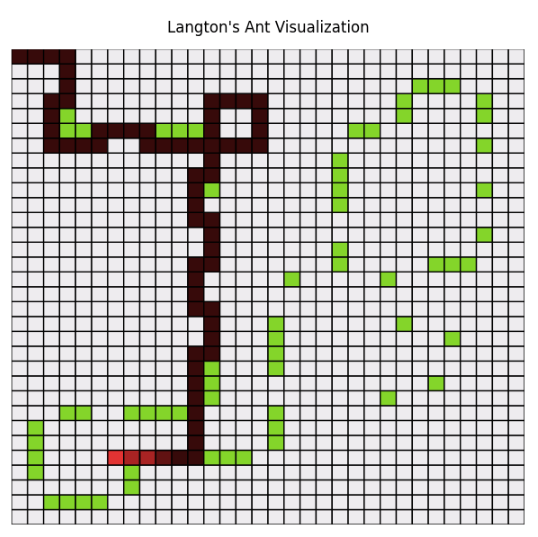
\includegraphics[scale=0.65]{obrazky-figures/ant-vis.png}
    \caption{Pokročilá vizualizace řešení}
    \label{fig:ant-vis}
\end{figure}


Zelená políčka v obr.~\ref{fig:ant-vis} reprezentují potravu, šedá políčka bez potravy, červená mravence a hnědá jeho cestu.
Jednotlivé obrázky se uchovávají ve složce \texttt{/images} a výsledný gif lze najít ve složce \texttt{/gif}. Aktivaci a deaktivaci je možné nastavit v~souboru \texttt{init\_params.py} u~parametru \texttt{CREATE\_GIF}.

\chapter{Experimentování}\label{ch:7}
Praktické části práce se věnuje právě tato kapitola, jež nejprve obsahuje obecný popis metod pomocí kterých jsou experimenty
statisticky vyhodnocovány a poté i následné experimenty. Ty se prvně zaměřují na
lineární GP (LGP), porovnání různých vylepšení, selekčních metod a taktéž hledání ideálních parametrů pro dané nastavení u~vybrané a náhodné stezky. Poté analogicky následuje stromové
GP (TGP) s~podobnými experimenty. Mezitím jsou taktéž srovnány obě varianty s~výsledky z~literatury. Nejsou zde bohužel zahrnuta všechna vylepšení a také kombinace různých nastavení,
která byla v~průběhu implementace nalezena a otestována z~důvodu již tak pravděpodobně
velkého rozsahu praktické části. Na závěr je o~těchto dalších vylepšeních, případně těch,
které se na první pohled zdály jako vylepšení, ale později se ukázalo, že algoritmus spíše
degradují, pojednáno.

\section{Způsob vyhodnocování experimentů}
Statistické vyhodnocování je prováděno a vizualizováno níže vysvětlenými metodami. \\

\noindent \textbf{Boxploty} 
\vspace{0.2cm} \\
Často jsou výsledky vizualizovány pomocí boxplotu, což je grafická reprezentace, která zobrazuje data na základě pětičíselného souhrnu. Ten se skládá z~minimální a maximální hodnoty, dolního (Q1) a horního (Q3) kvartilu a mediánu. Medián je reprezentován vertikální čárou uvnitř grafu, viz obr.~\ref{fig:boxplot}. Kvartily vyjadřují střední hodnotu mezi mediánem a nejmenší či největší hodnotou. Dále nám dokáže tato reprezentace říct, zdali jsou data symetrická, jejich rozptyl a variabilitu nebo jestli se v~nich nachází nějaké vyčnívající hodnoty (angl. \emph{outliers})~\cite{galarnyk_2022}.\\

\begin{figure}[!h]
    \centering
    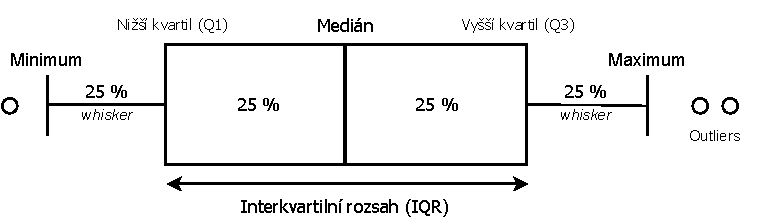
\includegraphics[scale=0.95]{obrazky-figures/boxplot.pdf}
    \caption{Vizualizace a popis boxplotu}
    \label{fig:boxplot}
\end{figure}
 
Dalším výsledkem experimentů jsou \textbf{konvergenční křivky}, jež vyjadřují grafické závislosti konvergence algoritmu na počtu iterací, tedy jak rychle se algoritmus přibližuje k~řešení. Posledním prostředkem k~vizualizaci je \textbf{tepelná mapa}, což je grafické zobrazení dat, ve kterém je každá hodnota reprezentována barvou určitého barevného spektra. Grafy v~následujících experimentech jsou zpracovány knihovnou \emph{matplotlib}.\\ 

\noindent Každá sada experimentů má definovanou skupinu stálých parametrů, které jsou shodné pro všechny testy v~této sadě. Tato tabulka obsahuje:
\begin{itemize}
    \item \emph{(jen LGP)} Uspořádanou pětici P = ($L_{min}, L_{max}, SR_{num}, SR_{min}, SR_{max}$) vyjadřující velikostní omezení programu, kde:
        \begin{description}
            \item $L_{min}$ -- minimální délka hlavního programu
            \item $L_{max}$ -- maximální délka hlavního programu
            \item $SR_{num}$ -- počet generovaných podprogramů
            \item $SR_{min}$ -- minimální délka podprogramu
            \item $SR_{max}$ -- maximální délka podprogramu
        \end{description}
    \item \emph{(jen TGP)} výškové omezení programu min. a max. hloubkou stromové struktury,
    \item inicializační metodu,
    \item selekční, rekombinační, mutační operátory,
    \item vybranou stezku (nahlédnutí na konkrétní stezku je možné ve zdrojových kódech v~souboru \texttt{trails\_plots.py}).
  
\end{itemize}

\noindent Pokud je experimentováno s~velikostí populace, tak je důležité, aby bylo dodrženo stejné velikosti prohledávaného prostoru k~najití nejlepšího řešení každému běhu, tzn. musí se zajistit, aby platila rovnice: \\

\begin{center}
    \fbox{\begin{minipage}{25em}
    \centering
    \textbf{velikost populace $\times$ počet generací = konstanta}
    \end{minipage}} 
\end{center} 
\bigskip
\noindent Pro všechny experimenty bude společná následující tab. parametrů~\ref{tab:params_all}.

\begin{table}[!h]
\centering
\begin{tabular}{ll}
\hline
\textbf{Parametry} &                                     \\
Cíl                & sesbírání veškeré potravy na mřížce \\
Fitness funkce     & standardizovaná                       \\
Elitismus          & ano                       \\
Počáteční pozice   & {[0, 0]}                          \\ \hline
\end{tabular}
\caption{Společné parametry pro všechny experimenty}
\label{tab:params_all}
\end{table}

\clearpage
\section{Experimenty}
\subsection{Vylepšení LGP I -- Motion Instruction Restriction}\label{subsection:2}

\begin{table}[!h]
\centering
\begin{tabular}{ll}
\hline
\textbf{Parametry}      &             \\
Délka programu       & P = (10, 15, 5, 4, 5)  \\
Stezka               & Santa Fe (max. fitness 89) \\
Inicializační metoda & náhodná s vel. omezeními  \\
Selekce              & turnajová          \\
Křížení              & jednobodové s P(0.5) \\
Mutace               & makro \& mikro s P(0.1)\\ 
Populace             & 100 \\ 
Generace             & 250 \\ \hline
\end{tabular}
\label{tab:6.3.3}
\caption{Parametry}
\end{table}

Toto vylepšení spočívá v~znemožnění algoritmu v~rámci genetického operátoru mutace v~podprogramech přidávat nebo nahrazovat jinou instrukci instrukcí \texttt{MOVE} (při inicializaci počáteční populace se v~podprogramech nadále nacházet může!). V~experimentu bylo spuštěno 60 nezávislých testů pro každé nastavení. 

\begin{figure}[!h]
    \centering
    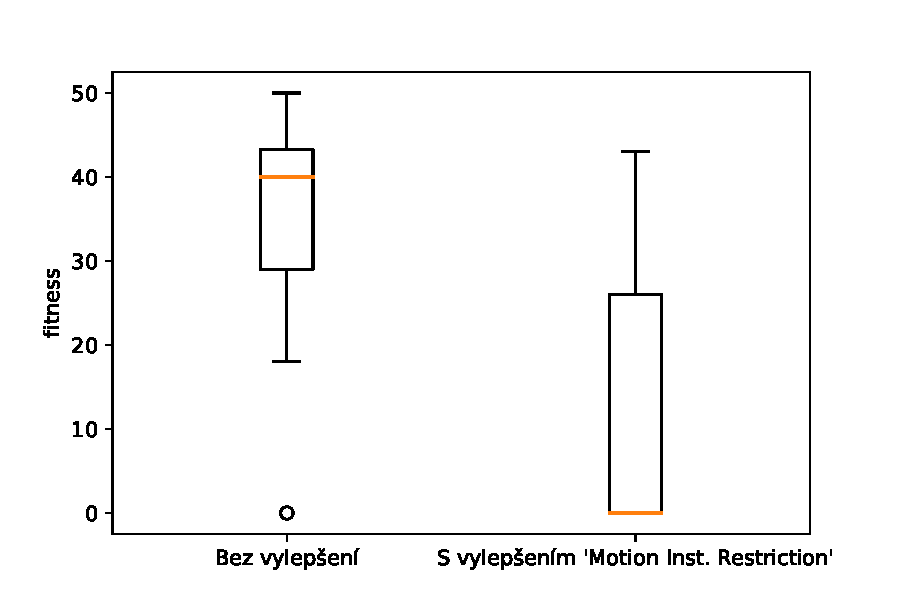
\includegraphics[scale=0.8]{obrazky-figures/exp-lgp-santafe-improvement-mut.pdf}
    \caption{Porovnání aplikovaného vylepšení}
    \label{fig:exp-lgp-santafe-improvement-mut}
\end{figure}

Z~výsledků testů na obr.~\ref{fig:exp-lgp-santafe-improvement-mut} je patrné, že i taková drobnost jako odstranění instrukce může učinit tak znatelný rozdíl ve výsledcích. 
Chvíli jsem nad tímto chování programu přemýšlel a dospěl jsem k~závěru, že je pro algoritmus mnohem snazší najít řešení, pokud dostane během evoluce více prostoru ke správnému nasměrování se v~rámci mřížky, než vykonávání ukvapených pohybů k~uražení co největší vzdálenosti, ale neefektivně. Často se tedy v~rámci hlavních programů vyskytují pouze jeden či dvě pohybové instrukce, které si s~úlohou hravě poradí, než kupříkladu deset pohybových instrukcí a minimum instrukcí k~určení směru pohybu. Dále z výsledků vyplynulo, že bez vylepšení se podařilo algoritmu najít řešení v~celkem 11 případech z~60, zatímco s~vylepšením v~36 případech. Nárůst řešení je tedy více než trojnásobný a pokles mediánu dokonce o~40 čísel!

\subsection{Vylepšení LGP II -- Grid Border Turn} 
\begin{table}[!h]
\centering
\begin{tabular}{ll}
\hline
\textbf{Parametry}   &             \\
Délka programu       & P = (10, 18, 6, 3, 4)  \\
Stezka               & Santa Fe (max. fitness 89) \\
Inicializační metoda & náhodná s vel. omezeními \\
Selekce              & turnajová  \\
Křížení              & jednobodové s P(0.4) \\
Mutace               & makro \& mikro s P(0.1)\\ 
Populace             & 100 \\ 
Generace             & 250 \\ \hline
\end{tabular}
    \caption{Paramtery}
\end{table}

Toto vylepšení spočívá v~tom, že pokud je mravenci znemožněn pohyb instrukcí \texttt{MOVE}, protože se nachází na hranici dvojdimenzionální mřížky, tak se pootočí o~90° ve směru hodinových ručiček. Toto opatření vkládá do pravidel určitou další diverzitu, která může znamenat najití lepších řešení. Pro každé z~obou variant bylo nezávisle spuštěno 4krát 40 testů, tedy 160 testů. Obě dvě varianty již zahrnují implementované rozšíření I.

\begin{figure}[!h]
    \centering
    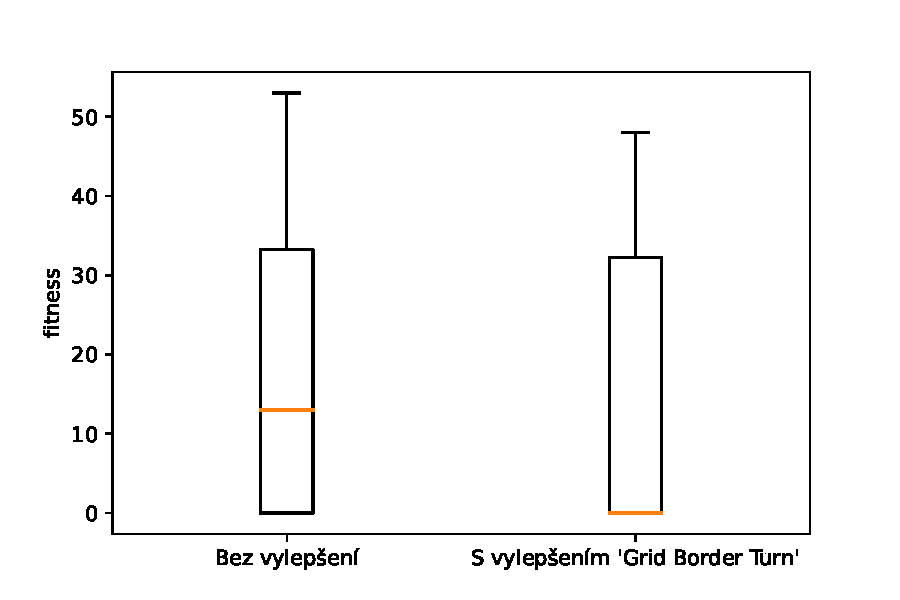
\includegraphics[scale=0.8]{obrazky-figures/exp-lgp-improvement-2-wall.pdf}
    \label{fig:exp-lgp-improvement-2-wall}
    \caption{Porovnání aplikovaného vylepšení, obě nastavení již implementují první vylepšení}
\end{figure}

Na první pohled je jasné, že se zdaleka nejedná o~tak markantní zlepšení jako v~případě prvního vylepšení, viz~\ref{subsection:2}. I~proto bylo provedeno mnohem více testů. Taktéž je dobré připomenout, že počáteční fixní hodnoty pro oba algoritmy se od předchozího, prvního, mírně liší. I~tak bylo dosaženo lepších výsledků. Hodnota mediánu se v~obou variantách mírně liší, konkrétně o~hodnotu 8 ve prospěch varianty s~vylepšením.


\subsection{Srovnání selekčních metod}
\begin{table}[!h]
\centering
\begin{tabular}{ll}
\hline
\textbf{Parametry}      &             \\
Délka programu       & P = (10, 15, 5, 4, 5)  \\
Stezka               & Santa Fe (max. fitness 89)\\
Inicializační metoda & náhodná s vel. omezeními \\
Selekce              & turnajová / ruleta / ranking \\
Křížení              & jednobodové s P(0.5) \\
Mutace               & makro \& mikro s P (0.1)\\ 
Populace             & 100 \\ 
Generace             & 250 \\ \hline
\end{tabular}
\caption{Parametry}
\end{table}

V~tomto experimentu jsem se zaměřil na porovnaní několika různých selekčních operátorů. Často je aplikován pouze operátor turnajový, ale co když existují i takové operátory, které si dokážou právě na této úloze vést lépe? Pro porovnání byla ještě kromě turnaje vybrána selekce ruletová a ranking. Pro každý níže zobrazený box plot bylo spuštěno 120 nezávislých běhů.

\begin{figure}[!h]
    \centering
    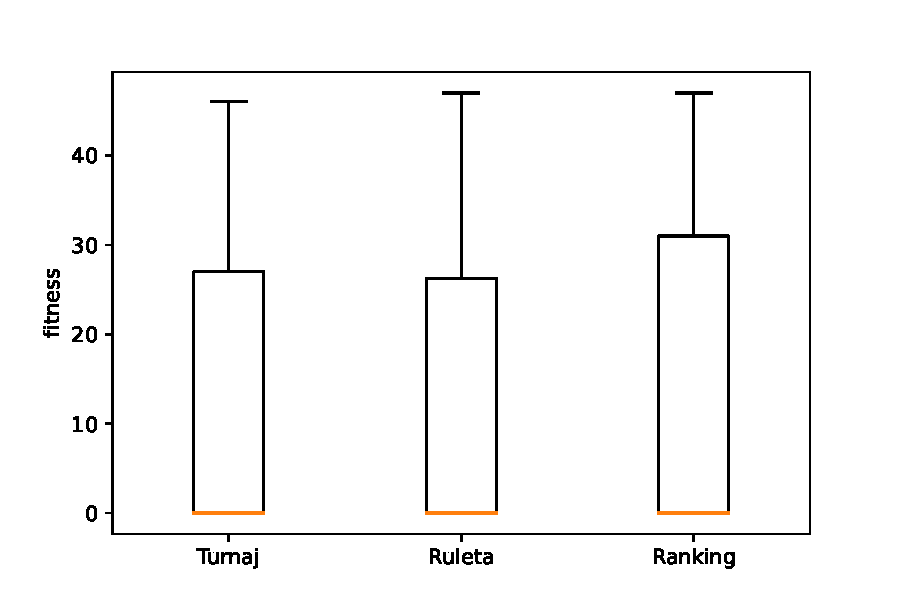
\includegraphics[scale=0.8]{obrazky-figures/exp-lgp-selection-met-comp.pdf}
    \caption{Výsledky experimentů selekčních metod}
    \label{fig:exp-lgp-selection-met-comp}
\end{figure}

Na obr.~\ref{fig:exp-lgp-selection-met-comp} lze vidět, že všechny operátory si s~touto instancí problému úspěšně poradily. Medián všech se drží na té nejlepší hodnotě. Menší výkyvy je možné zaznamenat ve~vyšších hodnotách, ačkoliv ani tyto rozdíly nejsou nikterak velké, 75 procent všech hodnot je nejmenších právě u~selekce ruletové. 
Konečné výsledky běhů ale nebyly pouze to jediné co mě zajímalo. Bohužel se u~tohoto problému neprojevila skutečnost zmíněná v~teoretické části, že některé z~těchto operátorů jsou náchylnější k~rychlejší konvergenci nebo v~nadměrném upřednostňování vhodnějších jedinců. Na všech vzorcích nebyl patrný větší rozdíl. U~turnajové selekce lze selekční tlak ještě ovlivnit nastavením velikostí počtu jedinců, jež do turnaje vstupují.

\subsection{Hledání ideálních parametrů LGP na vybrané stezce}\label{subsection:1}

\begin{table}[!h]
\centering
\begin{tabular}{ll}
\hline
\textbf{Parametry}      &             \\
Délka programu       & P = (10, 15, 5, 4, 5)  \\
Stezka               & Santa Fe (max. fitness 89)\\
Inicializační metoda & náhodná s vel. omezeními  \\
Selekce              & turnajová           \\
Křížení              & jednobodové \\
Mutace               & makro \& mikro \\ \hline
\end{tabular}
\caption{Parametry}
\end{table}  

Tento experiment již zahrnoval komplexnější hledání ideálního nastavení algoritmu. A~to konkrétněji u~tří parametrů -- velikosti populace, pravděpodobnosti křížení a mutace pro nalezení optimálního řešení. Nejprve byly testy spuštěny pro parametr populace, následně byl vybrán nejlepší výsledek, fixace této velikosti a analogickým postupem provedení stejného postupu i u~p. křížení a mutace. Bylo provedeno 120 nezávislých testů pro každé nastavení algoritmu. Tato i následující sady experimentů již zahrnují první implementované rozšíření. 

\begin{figure}[!h]
    \centering
    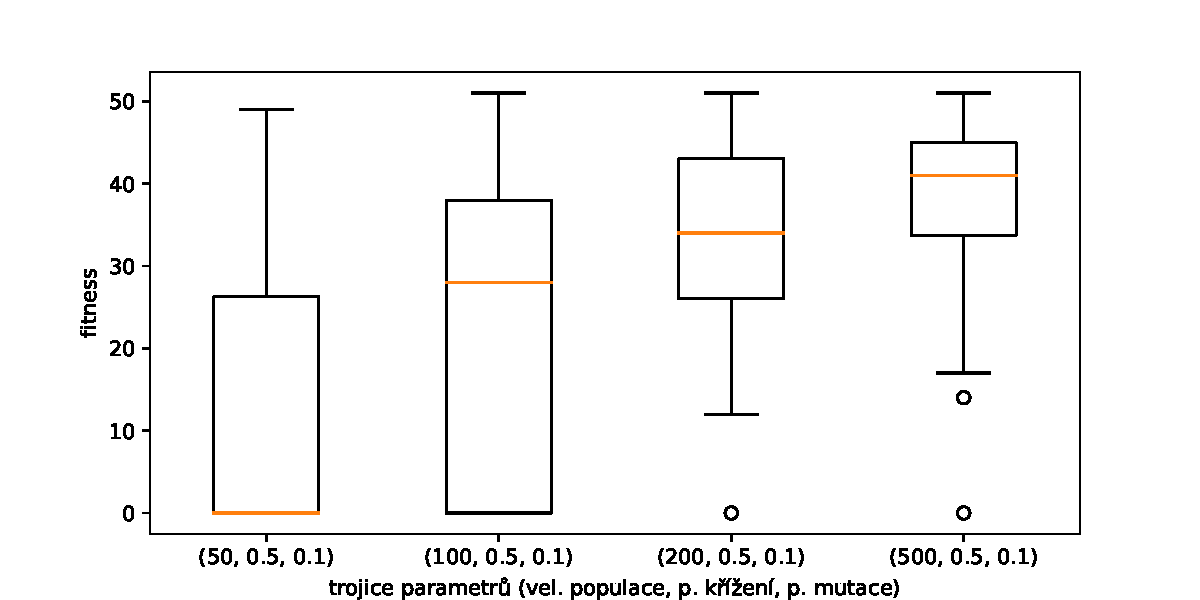
\includegraphics[scale=0.75]{obrazky-figures/exp-lgp-santafe-searching-params-1.pdf}
    \caption{Zjištění závislosti dosažené fitness na vel. populace}
    \label{fig:exp-lgp-santafe-searching-params-1}
\end{figure}

Z~grafu~\ref{fig:exp-lgp-santafe-searching-params-1} lze vidět, že řešení byla nalezena u~každé velikosti populace. Nejlepší výsledky byly obdrženy při nejmenší populaci. Podobného výsledku dosahuje i boxplot s~velikostí populace 100, ale již s~vyšším mediánem. Proto do dalšího spuštění programu byla zafixována velikost populace na 50 a zkoumán vliv různých hodnot pravděpodobnosti křížení. 

\begin{figure}[!h]
    \centering
    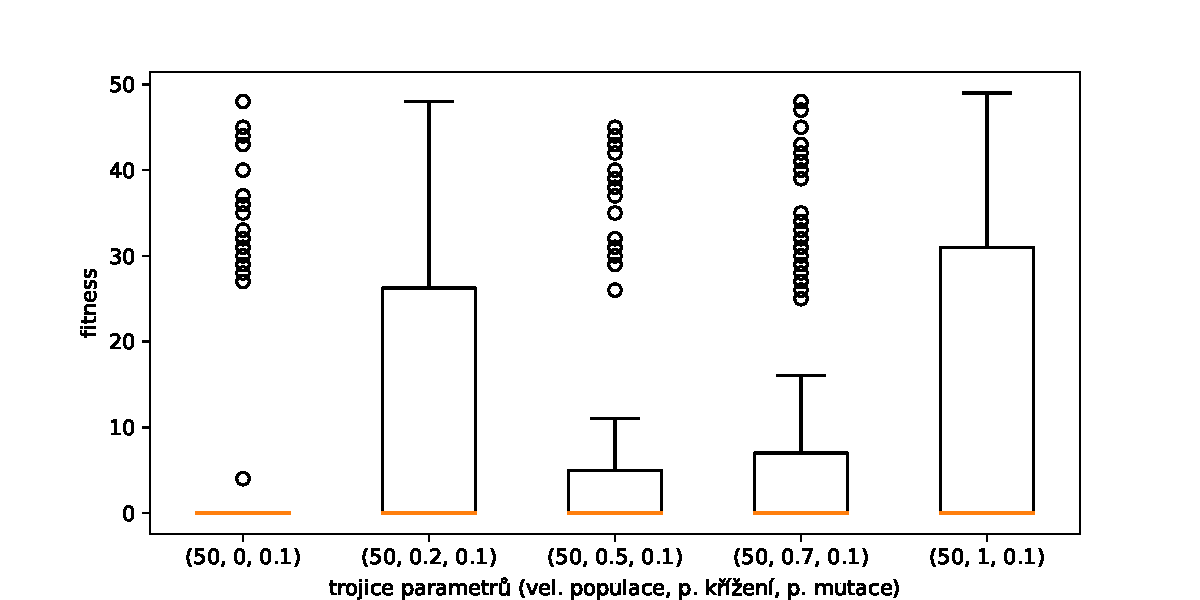
\includegraphics[scale=0.75]{obrazky-figures/exp-lgp-santafe-searching-params-2.pdf}
    \caption{Zjištění závislosti dosažené fitness na prav. křížení}
    \label{fig:exp-lgp-santafe-searching-params-2}
\end{figure}

Z~obr.~\ref{fig:exp-lgp-santafe-searching-params-2} je patrné, že medián se u~všech řešení nachází na hodnotě nula. Parametr pravděpodobnosti křížení byl zafixován pro první nastavení, protože se zde dosáhlo nejlepších výsledků. Ostatní nastavení pravidelněji dosahují vyšších hodnot fitness.

\begin{figure}[!h]
    \centering
    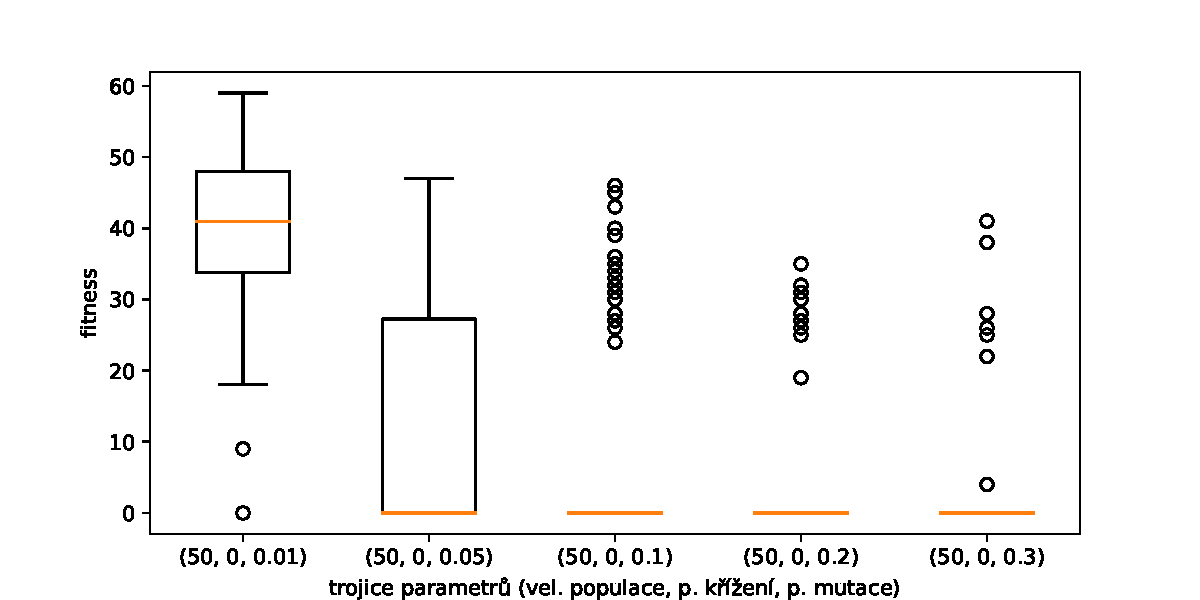
\includegraphics[scale=0.75]{obrazky-figures/exp-lgp-santafe-searching-params-3.pdf}
    \caption{Zjištění závislosti dosažené fitness na prav. mutace}
    \label{fig:exp-lgp-santafe-searching-params-3}
\end{figure}

U~prvního boxplotu, viz~\ref{fig:exp-lgp-santafe-searching-params-3}, je viditelné, že nulová pravděpodobnost křížení a velmi nízká pravděpodobnost mutace způsobila narůst mediánu. Již u~druhého nastavení bylo dosaženo viditelného pokroku. Nejlepších výsledků je dosahováno u~pravděpodobnosti 0.1, 0.2 a 0.3. Ty se již liší jen v~počtu a rozsahu odlehlých hodnot. Nejoptimálnějšímu výsledku proto vyhovují všechna tři poslední nastavení v~grafu. Celkově až na některé hodnoty variačních operátorů, které byly například u mutace nastaveny velice nízko, dosahovala ostatní řešení velice dobrých výsledků. Každé nastavení našlo minimálně jedno řešení. Je patrné, že výběr p. křížení zde nehrál tak zásadní roli jako při mutaci či velikosti populace. Je velice obdivuhodné, jak si tento algoritmus dokázal poradit s~touto instancí problému.

\subsection{Hledání ideálních parametrů LGP na náhodné stezce} 
\begin{table}[!h]
\centering
\begin{tabular}{ll}
\hline
\textbf{Parametry}      &             \\
Délka programu       & P = (8, 12, 5, 3, 5)  \\
Stezka               & Random Trail L (max. fitness 68) \\
Inicializační metoda & náhodná s vel. omezeními \\
Selekce              & turnajová       \\
Křížení              & jednobodové \\
Mutace               & makro \& mikro \\ 
\hline
\end{tabular}
\caption{Parametry}
\end{table}

Opět jako u předchozího experimentu byly zjišťovány nejlepší kombinace parametrů -- velikosti populace, pravděpodobnost křížení a mutace pro dosažení co nejlepších výsledků. Velikost dvojdimenzionální mřížky je opět 32 na 32 buněk, dohromady tedy 1024 buněk, z~čehož 68 tvoří náhodně rozmístěnou potravu.

\begin{figure}[!h]
    \centering
    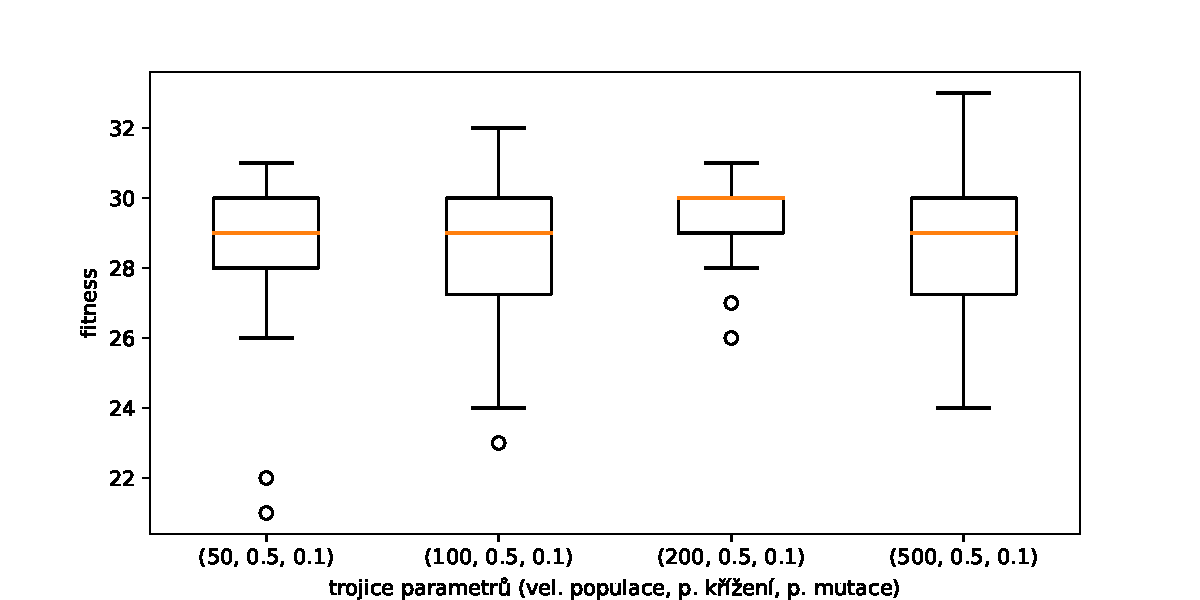
\includegraphics[scale=0.75]{obrazky-figures/exp-lgp-random-searching-params-1.pdf}
    \caption{Zjištění závislosti dosažené fitness na vel. populace}
    \label{fig:exp-lgp-random-searching-params-1}
\end{figure}

Na obr.~\ref{fig:exp-lgp-random-searching-params-1} lze vidět, že rozdíly ve výsledcích testů nejsou nikterak markantní, ale je zde pozorovatelné, že některá nastavení si vedla o~něco málo lépe než ostatní. Nejnižší fitness byla nalezena u~nastavení s~nejmenší populací, ale je to hodnota, která vybočuje. Velice se liší od ostatních hodnot u~tohoto nastavení. Proto pro další spuštění algoritmu byla vybrána varianta s~populací o~velikosti 100, kde minimální hodnoty dosahují častěji menších hodnot než u~předchozího nastavení. Varianta o~populaci 500 je zde na tom podobně, nejhůř dopadla varianta s~velikostí 200, kde se nachází velmi malý rozptyl získaných hodnot, které se ve většině případů pohybují okolo hodnoty fitness 28 až 30.  

Křížení na obr.~\ref{fig:exp-lgp-random-searching-params-2} opět nevykazuje velký vliv na získaná řešení, ale podařilo se nalézt opět o~něco lepší řešení, které dosahuje hodnoty fitness 20. Medián všech box plotů se zde ve většina případů až na malé desetinné odchylky rovná. Nejlepší minima, nepočítaje opět vyčnívající hodnoty, byla nalezena u~nastaveni křížení s~pravděpodobností 1, a proto bude i~toto nastavení použito pro další experimentování.

\begin{figure}[!h]
    \centering
    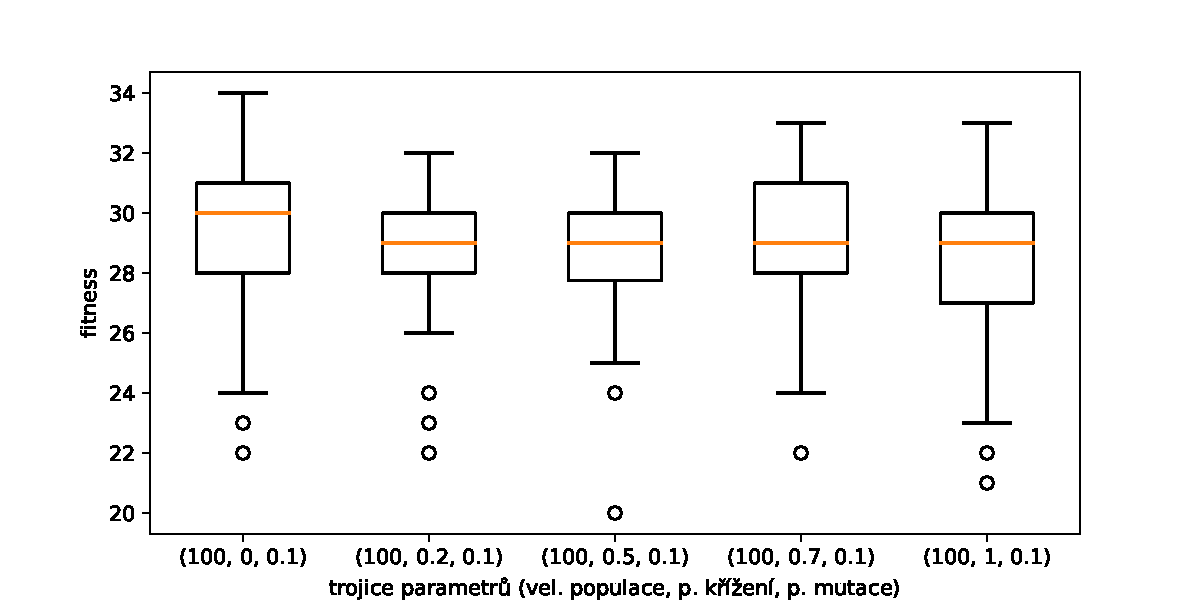
\includegraphics[scale=0.75]{obrazky-figures/exp-lgp-random-searching-params-2.pdf}
    \caption{Zjištění závislosti dosažené fitness na prav. křížení}
    \label{fig:exp-lgp-random-searching-params-2}
\end{figure}

Kombinace parametrů (100, 1, 0.01) na obr.~\ref{fig:exp-lgp-random-searching-params-3} bylo označeno jako nejlepší řešení a~to s~hodnotou fitness 16. Řešení s~vyšší pravděpodobnosti mutace si již nevedou tak dobře, jejich medián je oproti zbylým vyšší a rozptyl hodnot menší. 

\begin{figure}[!h]
    \centering
    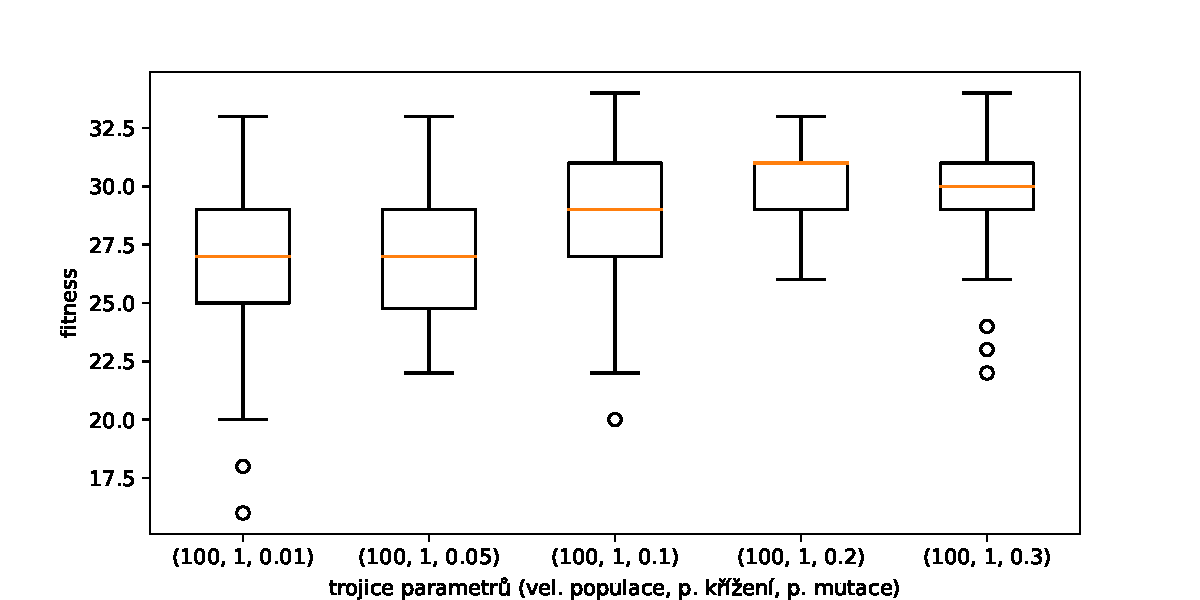
\includegraphics[scale=0.75]{obrazky-figures/exp-lgp-random-searching-params-3.pdf}
    \caption{Zjištění závislosti dosažené fitness na prav. mutace}
    \label{fig:exp-lgp-random-searching-params-3}
\end{figure}

Experimentování s~náhodnými stezkami je mnohem náročnější než s~těmi ideálními, které jsou především tvořené ze souvislých části obsahující pár menších či větších mezer. Pokud se náhodně na mřížce vyskytuje až příliš mnoho políček s~potravou, tak je velice nepravděpodobné nalézt řešení s~nejlepší fitness hodnotou, protože by často muselo dojít k~systematickému projití celé mřížky než najití nějakého schopného algoritmu s~co nejkratší cestou. Na druhou stranu, pokud se políček s~náhodně rozmístěnou potravou nachází na mřížce v~malém množství, tak sice nalezení takového programu, jenž by instanci tohoto problému zvládnul splnit je možné, ale opět to nebude snadné. Jedna z~klíčových vlastností tohoto algoritmu je podmíněnost, kde právě role políček s~potravou a podmíněných funkčních symbolů tvoří tu část, že se algoritmus nebude pokaždé chovat stejně. Terminální podmínky pro náhodné stezky jsou nadsazenější než u~ideálních, většinou na 40 \% projitých políček z~celé mřížky, což je optimální hodnota pro to, aby řešení nebylo tvořeno jen náhodnou procházkou, ale zároveň bylo poskytnuto dostatečné množství prostoru. Podobné testy byly provedeny i na menší mřížce (Random Trail S) o~velikosti 400 políček s náhodně rozmístněnou potravou. Zde si algoritmus vedl o~něco lépe, kde nacházel řešení průměrně v~5~bězích ze 40. V~bězích u~nichž se řešení nenašlo, se průměrná fitness pohybovala kolem 1 až 3.

\subsection{Porovnání s výsledky dostupnými v literatuře} 

Srovnání proběhlo na základě řešení dostupného v literatuře~\cite{Brameier1998} (str. 153 -- 155) s výsledky získanými s oběma variantami GP, u nichž byly vybrány jedny z nejlepších řešení. Obr.~\ref{fig:lit-santafe-example-tree} znázorňuje řešení, kterého bylo dosaženo za pomocí stromového GP v 21. generaci.

\begin{table}[h!]
\centering
\begin{tabular}{llll}
\hline
Parametry      & \multicolumn{1}{c}{Literatura TGP} & \multicolumn{1}{c}{LGP} & \multicolumn{1}{c}{TGP} \\ \hline
Délka programu & \emph{(nebylo zjištěno)}             & P = (6, 12,  5,  4,  5) & min. = 4, max. = 6 \\
Stezka         &  Santa Fe                          &  Santa Fe  &  Santa Fe                        \\ 
Populace       & 500                                & 100                     & 100   \\
Generace       & 51                                 & 120                     & 120   \\ \hline
\end{tabular}
\caption{Parametry}
\end{table}

\begin{figure}[!h]
    \centering
    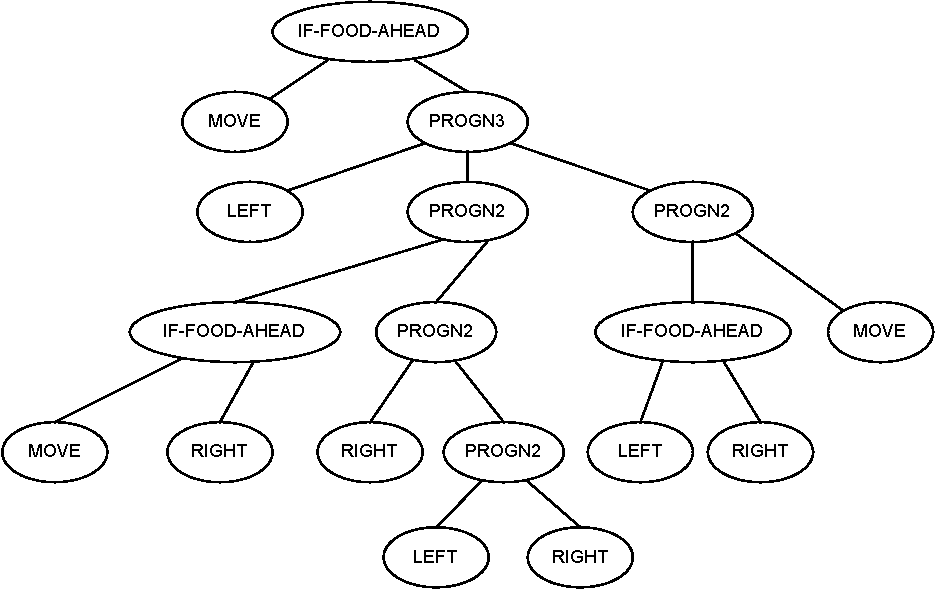
\includegraphics[scale=0.65]{obrazky-figures/lit-santafe-example-tree.pdf}
    \caption{Řešení uvedené v literatuře}
    \label{fig:lit-santafe-example-tree}
\end{figure}

Řešení je velice úsporné, dosahuje hloubky pět a k~pohybu mravence zde slouží 11 terminálních symbolů. Podmíněných uzlů se zde nachází tři, obzvláště ten v~kořenu stromu má zásadní vliv, jestli vykoná pouze instrukce \texttt{MOVE} nebo i~zbytek podstromu. Obr.~\ref{fig:lgp-santa-fe-comp-w-lit} značí mnou dosaženého řešení za pomocí lineárního GP v~22. generaci. Program se skládá z~hlavního programu obsahujícího 7 instrukcí, z~čehož většinu tvoří instrukce mravence a~2~ternární operátory. Šedou barvou jsou vyznačeny části kódu, resp. podprogramy, které se nikdy nevykonají. Je zajímavé, že celý program obsahuje pouze 3 instrukce \texttt{MOVE}, z~kterých je pouze jedna nepodmíněná a~evoluce taktéž upřednostnila podprogramy bez této instrukce, podprogramy A~ji totiž obsahuje. Obě zde zmíněná řešení splnila úlohu v~co nejkratší možnou dobu, tedy nejmenším počtu kroků.

\begin{figure}[]
    \centering
    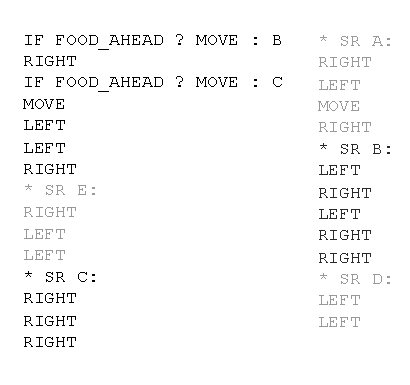
\includegraphics[scale=1]{obrazky-figures/lgp-santa-fe-comp-w-lit.pdf}
    \caption{Řešení nalezené lineárním GP}
    \label{fig:lgp-santa-fe-comp-w-lit}
\end{figure}

\newpage
\begin{figure}[!h]
    \centering
    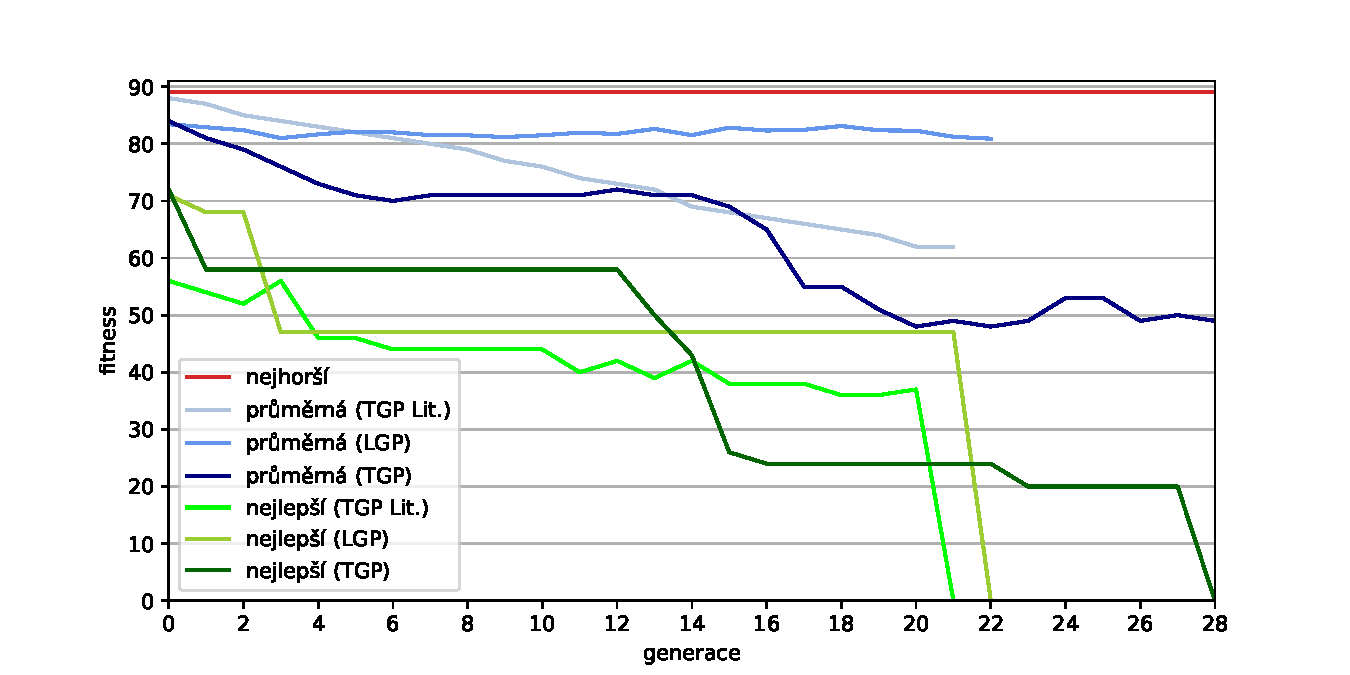
\includegraphics[scale=0.68]{obrazky-figures/lit-corv-curves.pdf}
    \caption{Konvergenční křivky s fitness hodnotami}
    \label{lit-corv-curves}
\end{figure}

Velikost a strukturu řešení získané vlastním programem stromového GP si je možné prohlédnout na přiloženém médiu ve složce s experimenty. 

Ačkoliv mé řešení stromového GP vykazuje o~trochu lepší výsledky průměrné fitness, tak trend klesající fitness na mnoha místech kopíruje křivku fitness hodnoty z~literatury, viz~\ref{lit-corv-curves}. Zajímavé hodnoty vykazuje řešení lineárního GP, kde fitness klesala markantněji pouze na začátku a poté byly zaznamenány pouze menší ojedinělé výkyvy. Řešení byla nalezena vcelku rychle. Lineární GP zde kopíruje křivku nejlepší fitness stromového GP z~literatury. Nejdéle trvalo najití řešení mé implementaci stromového GP. 

\clearpage
\subsection{Komplexní analýza parametrů TGP na vybrané stezce} 

\begin{table}[h!]
\centering
\begin{tabular}{ll}
\hline
\textbf{Parametry}  &                               \\ \hline
Velikost programů   & minimální = 3, maximální = 5 \\
Stezka              & Trail C (max. fitness 25)                     \\
Inicializační metoda & grow                          \\
Selekce             & turnajová                    \\
Křížení             & křížení se zarovnáním         \\
Mutace              & generující podstromy          \\ \hline
\end{tabular}
\caption{Parametry}
\label{tab:6.3.10}
\end{table}

\begin{table}[h!]
\centering
\begin{tabular}{lccccc}
\hline
\textbf{Populace}   & 50   & 100 & 200 & 500 & 1000 \\
\textbf{P(Křížení)} & 0.2  & 0.5 & 0.7 & 1   &      \\
\textbf{P(Mutace)}  & 0.01 & 0.1 & 0.2 & 0.5 & 1    \\ \hline
\end{tabular}
\caption{Analyzované hodnoty}
\label{tab:tgp-complex-params}
\end{table}

V~rámci tohoto experimentu byla provedena komplexní analýza všech třech parametrů a jejich hodnot zmíněných v~tab.~\ref{tab:tgp-complex-params}, tzn. důkladné testování všech možných trojic, které z~této tabulky můžou vzniknout ($5 * 4 * 5 = 100$ trojic). Pro každou trojici bylo provedeno 20 nezávislých běhů.

\begin{figure}[!h]
    \centering
    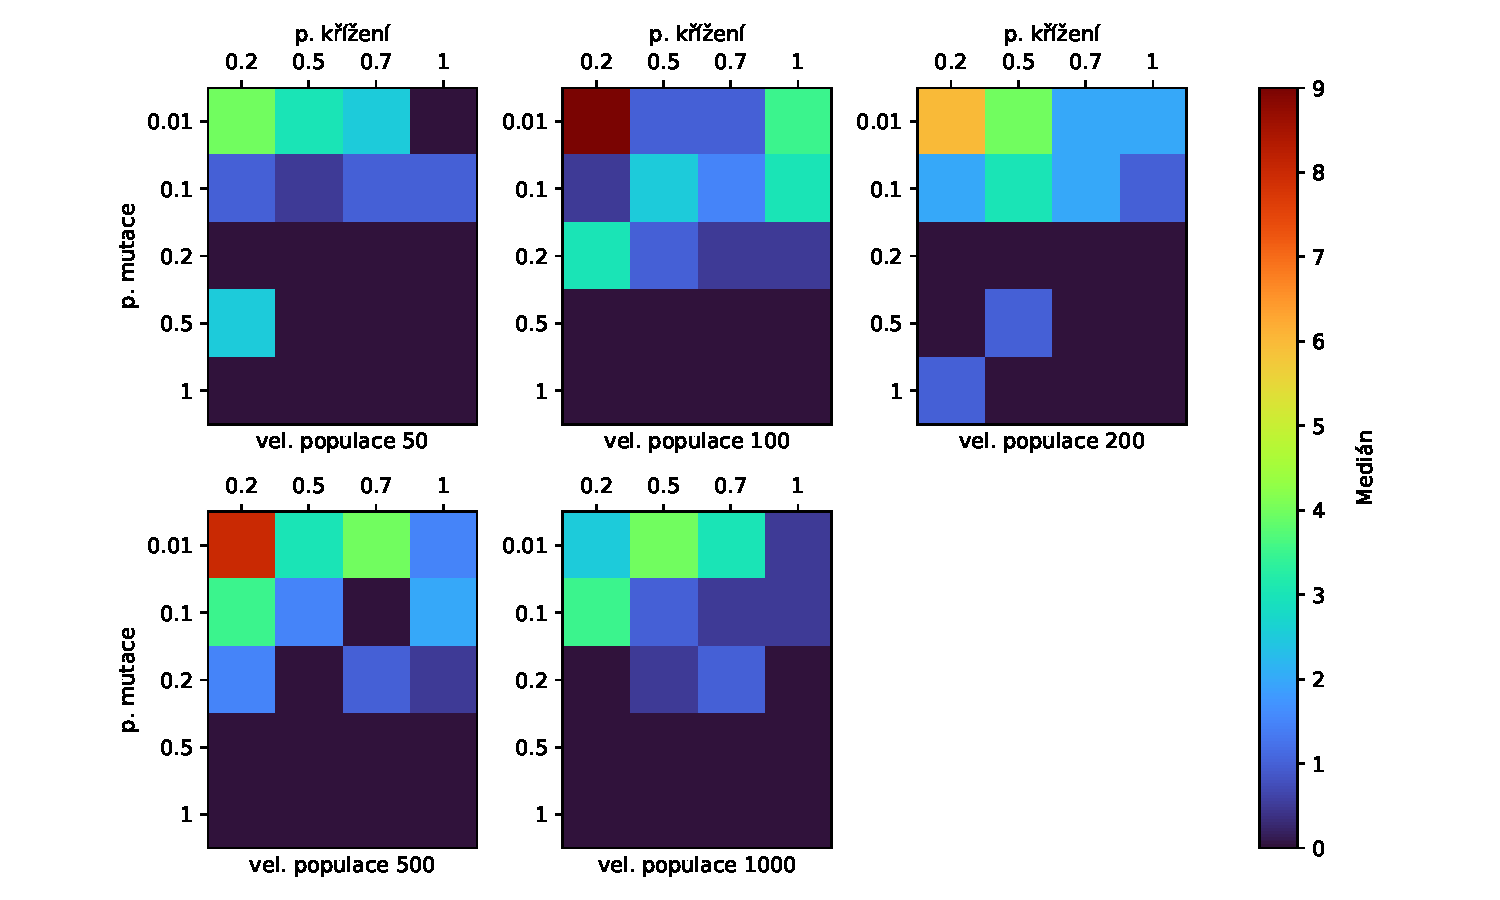
\includegraphics[scale=0.6]{obrazky-figures/tgp-20x20-heatmap.pdf}
    \caption{Teplotní mapy znázorňující velikost mediánu pro různé populace}
    \label{fig:gp-20x20-heatmap}
\end{figure} 


V~této práci je prezentována podrobněji pouze část experimentů z~důvodu rozsáhlosti, která by tato analýza spotřebovala. Hodnota mediánu všech sad je vyobrazena na obr.~\ref{fig:gp-20x20-heatmap}. Experimenty jsou rozděleny do 5 skupin (každá o různé populaci), vždy po 20 boxplotech. Pro podrobnější prezentaci bylo vybráno nastavení s~velikostí populace 500, viz obr.~\ref{fig:exp-tgp-20x20-pop500.pdf}. Osa \emph{x} je vždy popsána  kombinací parametrů pro které byla sada experimentů spuštěna. Tučně je vyznačen parametr shodný pro danou pětici sad, v tomto případě pravděpodobnost křížení. V každé této pětici se následně ještě mění pravděpodobnost mutace. U~všech 4~pětic se opakoval obdobný trend, viz obr.~\ref{fig:exp-tgp-20x20-pop500.pdf}, že řešení s~větší pravděpodobností mutace ($\geq 0.5$), nezávisle na křížení, dosahovala lepších výsledků povětšinou mediánu s~hodnotou 0~a malým počtem hodnot s vysokou fitness, než řešení naopak s~menší pravděpodobností. Největší medián je k~spatření u~nejmenší hodnoty křížení. Taktéž nezávisle na populaci, viz obr.~\ref{fig:gp-20x20-heatmap}, se zde nikterak neprojevila výhoda větší či menší populace i s tím, že každé z~nich byl poskytnut stejný prohledávací prostor řešení. Závěrem lze tedy říct,  že mutace se z~tohoto experimentu jeví jako silnější operátor než křížení majícího vliv na kvalitu výsledného řešení.

\bigskip
\bigskip
\bigskip

\begin{figure}[!h]
    \centering
    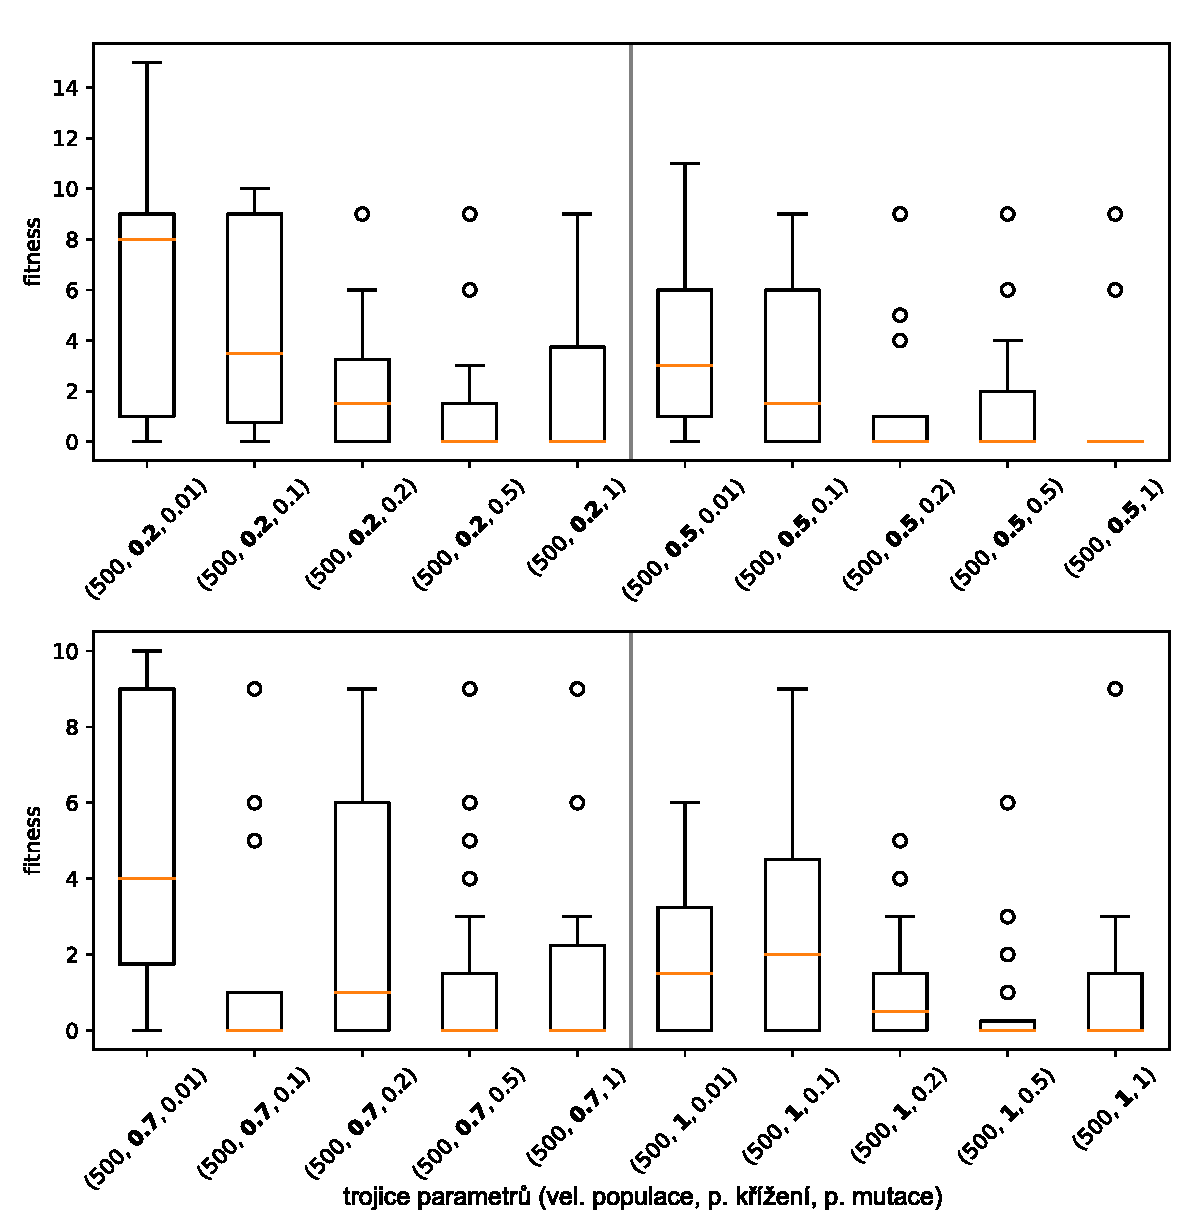
\includegraphics[scale=0.7]{obrazky-figures/exp-tgp-20x20-pop500.pdf}
    \caption{Vybraná skupina experimentů se stejnou velikostí populace}
    \label{fig:exp-tgp-20x20-pop500.pdf}
\end{figure} 


\newpage
\subsection{Hledání ideálních parametrů TGP na vybrané stezce}\label{subsection:3} 
\begin{table}[h!]
\centering
\begin{tabular}{ll}
\hline
\textbf{Parametry}  &                               \\ \hline
Velikost programů   & minimální = 4, maximální = 6 \\
Stezka              & Santa Fe (max. fitness 89)     \\
Inicializační metoda & grow                          \\
Selekce             & turnajová                     \\
Křížení             & křížení se zarovnáním         \\
Mutace              & generující podstromy          \\ \hline
\end{tabular}
\caption{Parametry}
\label{tab:6.3.9}
\end{table}
%max 100 000 vyhodnoceni fitness
Obdobně jako v~experimentu~\ref{subsection:1} byly hledány ideální parametry (velikost populace, p.~křížení a p.~mutace) algoritmu pro  hodnoty v~tab.~\ref{tab:6.3.9}. Ačkoliv velikostní omezení programu je jen o~jedničku vyšší ve srovnání s~minulým experimentem, což se může zdát pro již takto komplexnější úlohu málo, tak toto omezení nebere v~potaz šířku řešení, tzn. stromu, které může být neomezené. Tyto výsledky budou následně použity pro porovnání s~lineárním GP. Pro každé nastavení bylo spuštěno 120 nezávislých běhů.

\begin{figure}[!h]
    \centering
    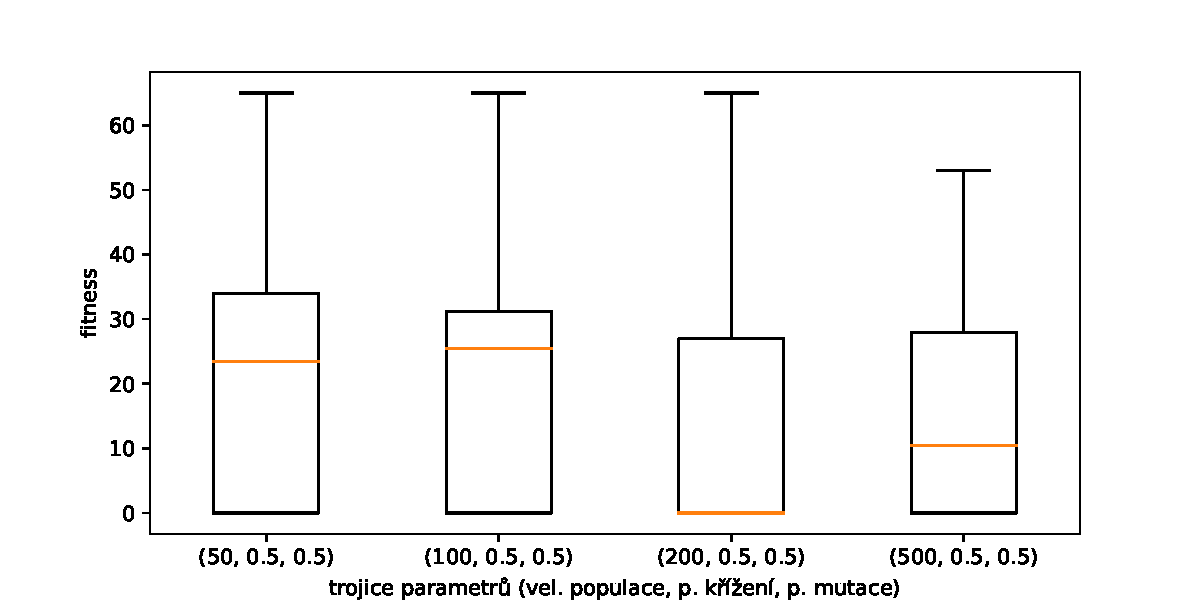
\includegraphics[scale=0.65]{obrazky-figures/exp-tgp-santfe-searching-params-1.pdf}
    \caption{Zjištění závislosti dosažené fitness na velikosti populace}
    \label{fig:exp-tgp-santa-fe-1}
\end{figure} 

Všechna nastavení úspěšně našla několik řešení, ale jejich medián se poněkud liší. Za nastavením s~populací 200 značně pokulhávají první dvě nastavení. Všechna řešení si taktéž udržují vyšší hodnoty maximální fitness v porovnání s lineárním GP v~experimentu~\ref{subsection:1}. Všechna data jsou ale konzistentní, žádné hodnoty nevybočují. Pro další experimenty bylo vybráno nastavení s~populací 200 z~důvodu nejnižší hodnoty mediánu.

\begin{figure}[!h]
    \centering
    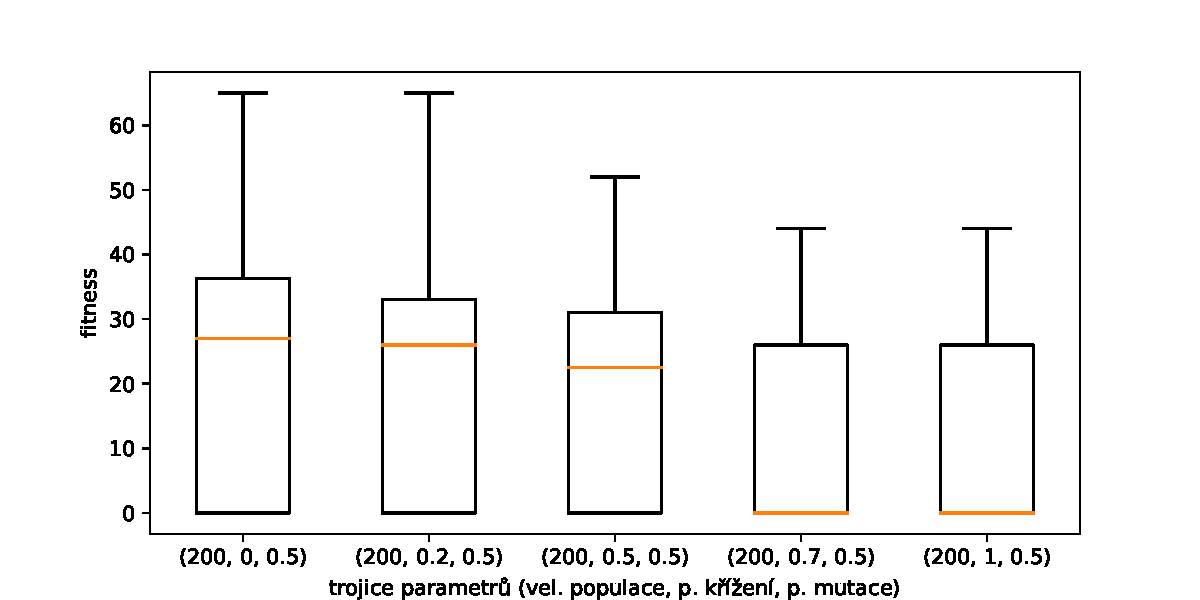
\includegraphics[scale=0.65]{obrazky-figures/exp-tgp-santfe-searching-params-2.pdf}
    \caption{Zjištění závislosti dosažené fitness na pravděpodobnosti křížení}
    \label{fig:exp-tgp-santa-fe-2}
\end{figure} 

Na obr.~\ref{fig:exp-tgp-santa-fe-3} lze vidět již tendenci mediánu klesat se zvyšující se pravděpodobností křížení. Poněkud větší skok lze vidět mezi pravděpodobnostmi 0.5 a 0.7. Skoro až identicky se podobají řešení s~dvěma nejvyššími pravděpodobnostmi, náhodně jsem proto do dalšího experimentování vybral tu variantu s~hodnotou 0.7.

\newpage
\begin{figure}[!h]
    \centering
    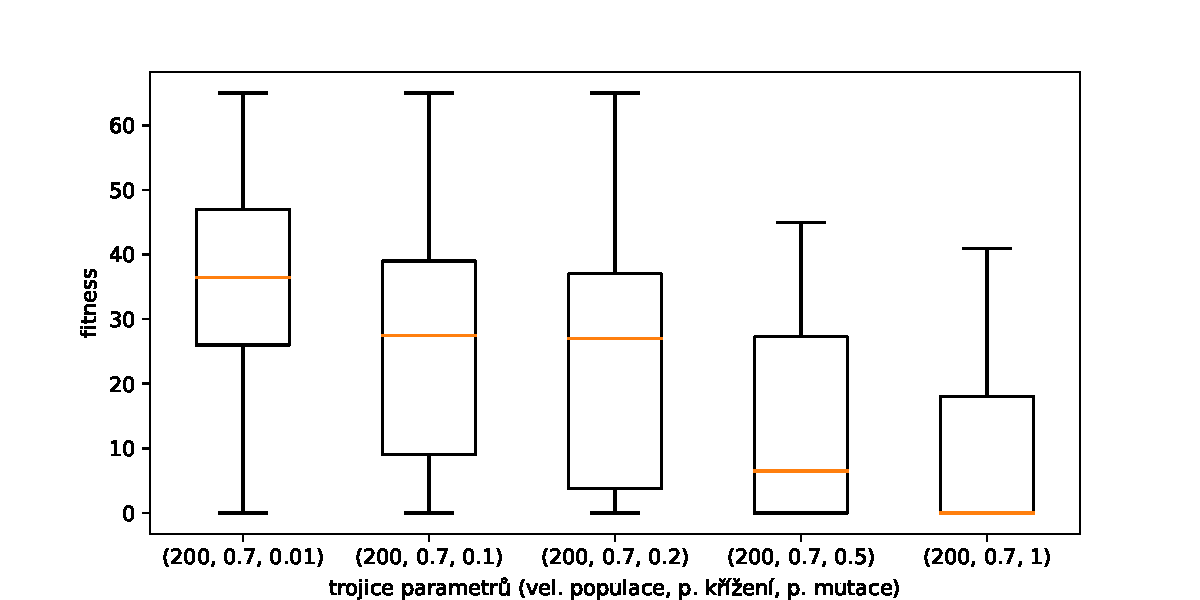
\includegraphics[scale=0.65]{obrazky-figures/exp-tgp-santfe-searching-params-3.pdf}
    \caption{Zjištění závislosti dosažené fitness na pravděpodobnosti mutace}
    \label{fig:exp-tgp-santa-fe-3}
\end{figure}    

Různé pravděpodobnosti mutace přináší do řešení ještě větší diverzitu. Na rozdíl od obr.~\ref{fig:exp-tgp-santa-fe-2}, kde se 75 \% všech hodnot nacházelo mezi hranicí prvního a třetího kvartilu, zde u~prvních třech boxplotech a~zejména toho prvního lze pozorovat opět důležitost tohoto operátoru a to jak se fitness zhorší, pokud se operátor vyskytuje s velice malou pravděpodobností. Nejlepším řešením se tedy osvědčila kombinace parametrů (200, 0.7, 0.1), kde jako u jediné kombinace parametrů se medián nachází na hodnotě 0.

\clearpage
\subsection{Srovnání stromového a lineárního GP}
V rámci tohoto srovnání stromového a lineárního GP bylo primárně vycházeno z experimentů z podkapitol~\ref{subsection:1} a~\ref{subsection:3}, konkrétně z nastavení, které poskytovalo nejlepší výsledky. U lineárního GP kombinace parametrů (50, 0, 0.2) (obr.~\ref{fig:exp-lgp-santafe-searching-params-3}), u stromového GP (200, 0.7, 1) (obr.~\ref{fig:exp-tgp-santa-fe-3}). Pro každé toto nastavení bylo provedeno 120 nezávislých testů, ze kterých vzejde hlubší statistické vyhodnocení.

\begin{table}[!h]
\centering
\begin{tabular}{|l|l|l|}
\hline                               & \textbf{TGP} & \textbf{LGP} \\ \hline
\textbf{počet testů}                 & 120          & 120          \\ \hline
\textbf{$\sum$ fitness}          &   1067         &  	281            \\ \hline
\textbf{$\varnothing$ fitness}                   & 8.89         & 2.34             \\ \hline
\textbf{↑ max. fitness}              & 41           &  35            \\ \hline
\textbf{↓ min. fitness}              & 0            &  0            \\ \hline
\textbf{modus (počet)}              & 0 (70)       &  0 (110)           \\ \hline
\end{tabular}
\caption{Statistické porovnání stromového (TGP) a lineárního (LGP) GP}
\label{tab:stats-tgp-lgp-comp}
\end{table}

Již na první pohled tab.~\ref{tab:stats-tgp-lgp-comp} je znatelné, že se  varianty v~úspěšnosti řešení této úlohy velice liší. Nepatrné odlišnosti lze vidět nejen u~součtu celkové hodnoty fitness, ale taktéž u~počtu nalezených řešeních. To se v~případě lineárního GP podařilo téměř u~každého běhu. Maximální fitness hodnota se u~obou variant je velice podobá, za to průměrná fitness je u~varianty lineárního GP až 4krát nižší.

\begin{figure}[!h]
    \centering
    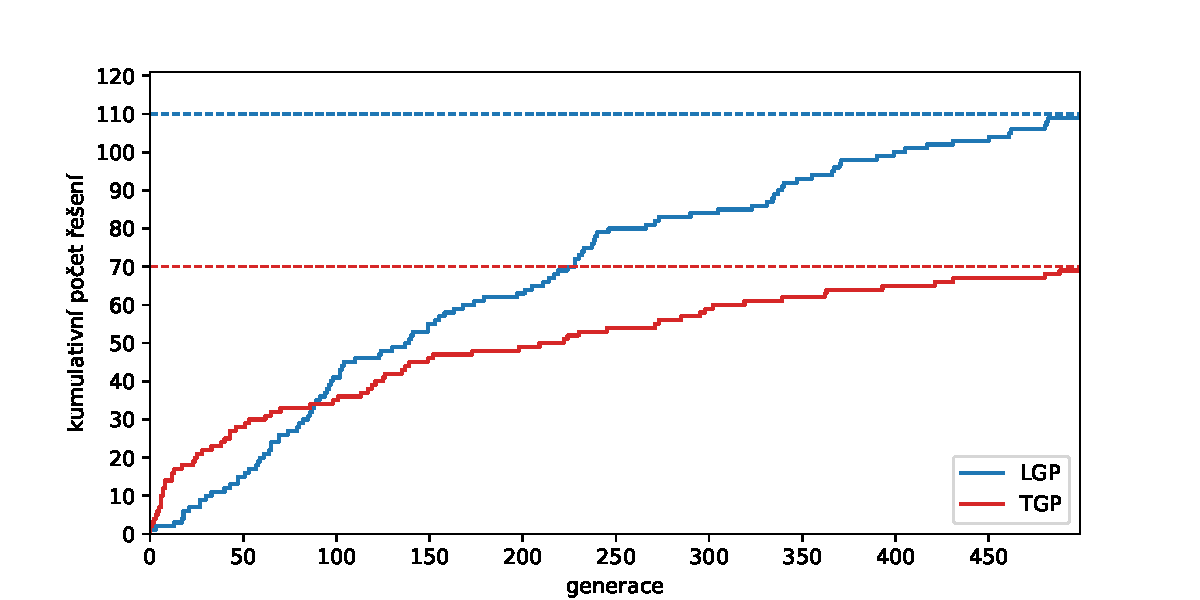
\includegraphics[scale=0.7]{obrazky-figures/tgp-lgp-comp-cumulative.pdf}
    \caption{Graf zobrazující generace a počet dosud získaných řešení v každé generaci ze všech spuštěných běhů.}
    \label{fig:tgp-lgp-comp-cumulative}
\end{figure}

Graf~\ref{fig:tgp-lgp-comp-cumulative} znázorňující generace na ose \emph{x} a počet celkově dosud získaných řešení na ose \emph{y} v dané generaci z celkově 120 nezávislých běhů. Na počátku lze vidět, že si běhy stromového GP vedou s~větší populací jedinců lépe. Téměř 30 běhům se podařilo najít řešení do 50 generací, zatímco u~lineárního GP pouze 10 běhům. Zlom nastává po cirka sto generacích, kdy přírůstek již dostává pomalejšího charakteru. Rychlost nalezení řešení lineárního GP se zdá býti až na menší občasné výkyvy konstantní.

\newpage
Dále byly pro toto srovnání spuštěny sady nezávislých testů o~10 bězích pro každou variantu GP. Následující dva grafy znázorňují konvergenční křivky průměrné a nejlepší fitness.

\begin{figure}[!h]
    \centering
    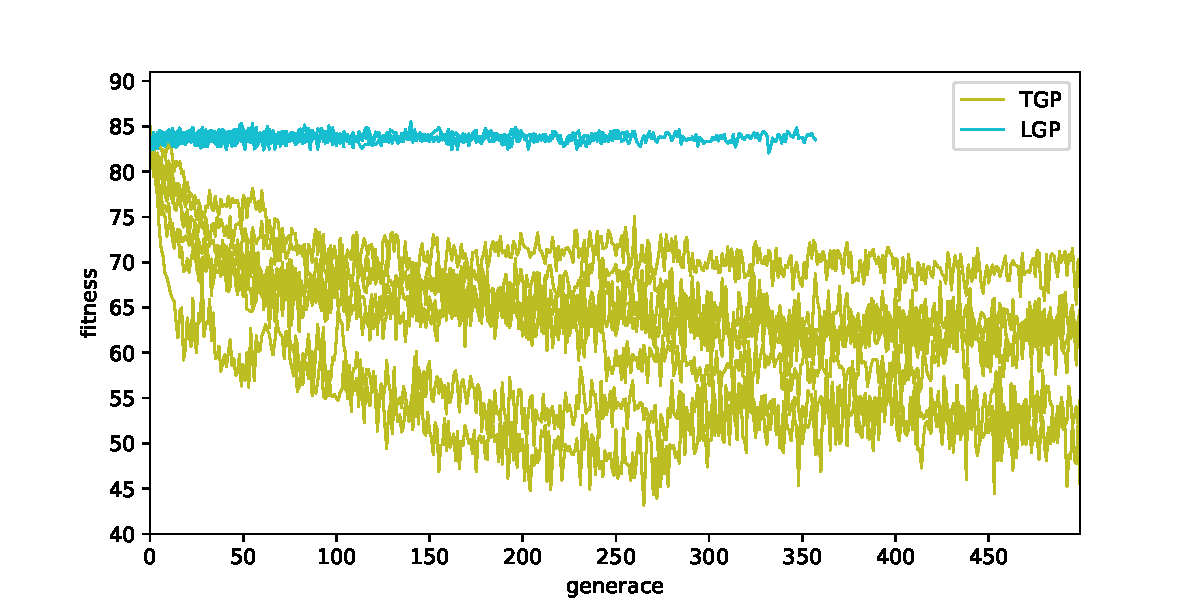
\includegraphics[scale=0.7]{obrazky-figures/tgp-lgp-comp-avg-fitness.pdf}
    \caption{Průměrná fitness
    }
    \label{fig:tgp-lgp-comp-avg-fitness}
\end{figure}  

Z~grafu~\ref{fig:tgp-lgp-comp-avg-fitness} lze vidět, že chování průměrné fitness je u~obou variant velmi rozdílné a~zároveň i~velmi podobné tomu, co bylo prezentováno v~podkapitole ve srovnání s~literaturou, viz obr.~\ref{lit-corv-curves}. Zatímco u~stromového GP fitness hodnota v~průběhu generací klesá, tak u~lineárního GP lze pozorovat velmi podobný model chování u všech běhů, tedy fluktuaci s~velmi ojedinělými výkyvy. 

\begin{figure}[!h]
    \centering
    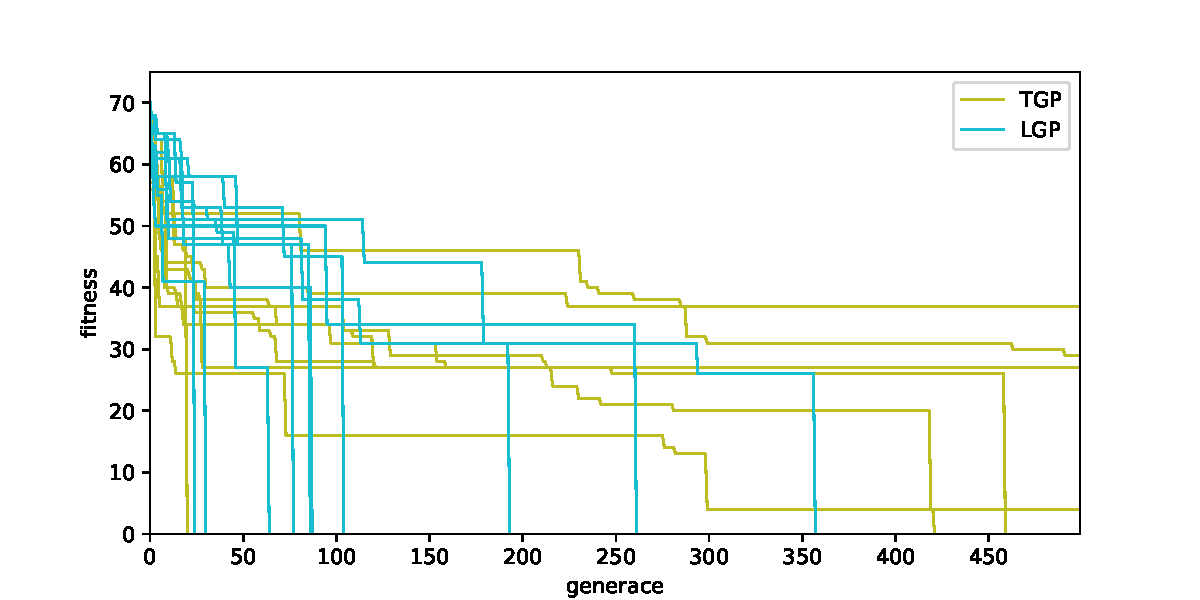
\includegraphics[scale=0.7]{obrazky-figures/tgp-lgp-comp-best-fitness.pdf}
    \caption{Nejlepší fitness}
    \label{fig:tgp-lgp-comp-best-fitness}
\end{figure}  

Graf~\ref{fig:tgp-lgp-comp-best-fitness} zobrazuje hodnoty nejlepších fitness hodnot v průběhu generací. Zatímco lineárnímu GP se podařilo vyřešit úlohu v každém z deseti běhů, tak u stromového GP bylo nalezeno řešení pouze u čtyř běhů (pozn. první řešení bylo nalezeno již v nulté generaci, které bohužel nelze v grafu vidět). Ke konvergenci zde dochází pomaleji oproti lineárnímu GP. Většina řešení byla u lineárního GP nalezena poměrně rychle a~lze u~nich pozorovat v~prvních generacích vcelku svižný pokles fitness hodnot.

\subsection{Srovnání variant operátorů křížení u TGP}

\begin{table}[h!]
\centering
\begin{tabular}{ll}
\hline
\textbf{Parametry}  &                               \\
Velikost programů   & minimální = 4, maximální  = 6 \\
Stezka              & Santa Fe (max. fitness 89)                    \\
Inicializační metoda & grow                          \\
Selekce             & turnajová                     \\
Mutace              & generující podstromy s P(1)         \\ 
Populace              & 200         \\ \hline
\end{tabular}
\caption{Parametry}
\label{tab:tba}
\end{table}

V tomto posledním experimentu byly porovnány varianty operátoru křížení, jež různě přistupují k řešení problému \emph{bloatu}, které s touto variantou GP souvisí. Bez nich by totiž docházelo k~tvorbě řešení s neomezenou velikostí. Pro porovnání byly vybrány následující dvě varianty:

\begin{itemize}
    \item \textbf{Cross \& Cut} -- Metoda po křížení zkontroluje výšku řešení a případně jej na tuto výšku zarovná terminálními symboly. Využívána v předchozích experimentech u stromového GP.
    \item \textbf{Double Cross, Mutate \& Cut} -- Provede křížení, zkontroluje výšku, v případě že výška není dodržena provede s původním rodičem opětovné křížení, analogicky opět zkontroluje výšku a pokud stále nevyhovuje velikostním omezením, tak je provedena mutace s případným zarovnáním.
\end{itemize}

\begin{figure}[!h]
    \centering
    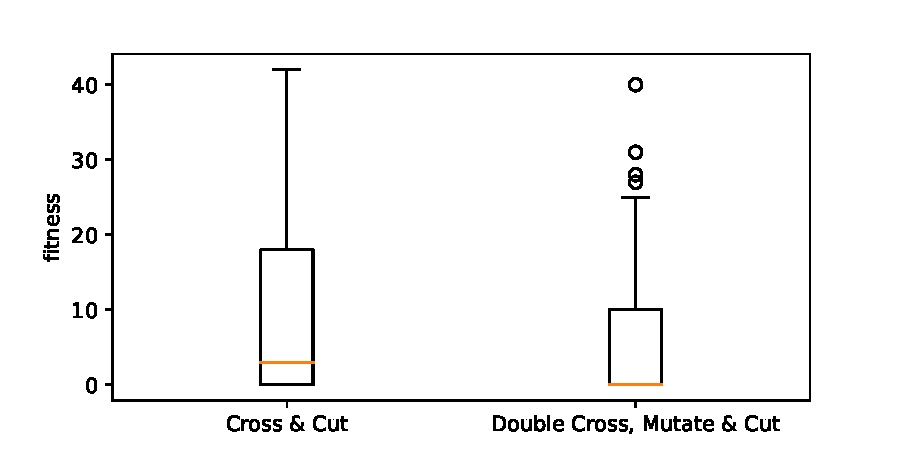
\includegraphics[scale=0.9]{obrazky-figures/exp-tgp-cross-comp.pdf}
    \caption{Porovnání fitness hodnot obou variant křížení (obě s P(0.7))}
    \label{fig:exp-tgp-cross-comp}
\end{figure}  

Z výsledků z obr.~\ref{fig:exp-tgp-cross-comp} vyplynulo, že si druhá varianta křížení vede o mnoho lépe. Obě techniky dosahují téměř podobného mediánu, ale liší se v hranicích třetího kvartilu a taktéž maximálních hodnotách (nepočítaje vyčnívajících hodnot). Druhá varianta je ale výpočetně mnohem složitější. Pro další porovnání bylo spuštěno dalších 20 nezávislých testů s modifikovanou pravděpodobností křížení na hodnotu 1, aby byla zaručena co největší rovnoměrnost oběma variantám. U těchto testů byla změřena výpočetní náročnost operátoru křížení u~celé jedné generace, tyto hodnoty následně sečteny a zprůměrovány.

\begin{figure}[!h]
    \centering
    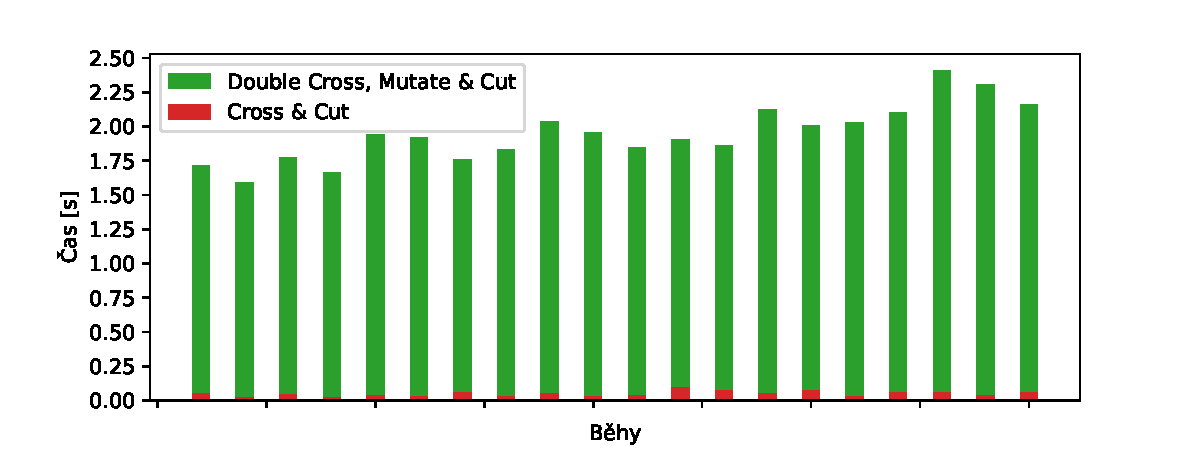
\includegraphics[scale=0.7]{obrazky-figures/exp-tgp-cross-comp-time.pdf}
    \caption{Porovnání výpočetní náročnosti obou variant křížení}
    \label{fig:exp-tgp-cross-comp-time}
\end{figure}  

Z grafu~\ref{fig:exp-tgp-cross-comp-time} se jasně potvrdilo, že ačkoliv druhá varianta jasně prokazovala lepší výsledky, tak je vzniká otázka, zdali se i za cenu výpočetní náročnosti obecně vyplatí využívat pokročilejší varianty těchto operátorů. Zrovna křížení u stromových struktur není levná záležitost. Celkový výpočetní čas u první varianty činil \textbf{0.659 s}, zatímco u druhé \textbf{35.937 s}. Při velkých populacích a generacích tento rozdíl samozřejmě narůstá. Je zde ale stále spousta faktorů, která výsledný čas můžou ovlivnit jako je například počáteční populace. V~závěru plyne, že obě varianty si úspěšně poradily s problémem \emph{bloatu}, jedna varianta vykazuje mnohem větší náročnost než druhá, ale také než pouze na těchto číselných hodnotách také závisí na zvolené instanci problému a věcech, které není možné ovlivnit (např. vygenerovanou počáteční populaci).


\section{Další modifikace }
V rámci obou technik GP byla v průběhu vývoje implementována a testována spousta dalších modifikací, které už z důvodu rozumného rozsahu praktické části této práce zde nebyly zahrnuty. Mezi jedno z nich by se například dalo zařadit změna počáteční pozice mravence. Samozřejmě ne všechny modifikace vykazovaly zlepšení, některé algoritmy přímo degradovaly. \\

\noindent\textbf{Neúspěšná vylepšení} \\
Při experimentování ve snaze dalšího zlepšení obou variant GP byla nalezena i neúspěšná vylepšení, která se na první pohled jevila, že by mohli mít na řešení pozitivní vliv. Nebudu je tu nikterak do detailu porovnávat, ale chci se o nich alespoň krátce zmínit.

Jedno z prvních neúspěšných vylepšení bylo umožnění mravenci pohybovat se namísto čtyř v osmi směrech, tzn. pohyb i v rámci diagonál. Ačkoliv bylo zamýšleno, že by se mravenec mohl více citlivěji pohybovat, lépe se směrovat a reagovat i na potravu, která se může nacházet v diagonálním směru, tak vyústilo v celkový zhoršený pohyb. Modelový příklad, mravenec se chce otočit o 180°, namísto původních dvou instrukcí které k tomuto stačily, tak by byly teď potřeba čtyři. Byla testována i varianta v přidání nových instrukcí, které by diagonální pohyb umožňovali a zachování těch původních, aby byla omezena četnost pohybu v osmi směrech. Ani toto zlepšení neprokázalo dostatečně dobré výsledky.
Mezi další takovéto degradace algoritmu lze zařadit nový terminální symbol \texttt{JUMP}, který umožňuje mravenci obskočit jedno políčko. Opět tu je nutná velká regulace, aby se tato instrukce nevyskytovala v řešeních často. Původní zamyšlení bylo možnost prohledávat prostor různých řešeních rychlejším způsobem. \\

\noindent\textbf{Možná další vylepšení} \\
Mezi další vylepšení lze uvažovat například optimalizaci GP. Často se v programu vyskytuje skupina instrukcí, jež nikterak neovlivňují výslednou pozici mravence. Na obr.~\ref{fig:optimalization} jsou uvedeny příklady z každé varianty GP. Například skupina čtyř instrukci \texttt{LEFT} uvede mravence do stejného stavu jako před jejich vykonáním. Přidáním instrukce \texttt{NOP}, jež by nevykonávala žádnou operaci by mohlo dojít až ke čtyřnásobnému ušetření času, obzvláště u komplexních problému my mohlo dojít ke zlepšení a celkové optimalizaci.

\begin{figure}[!h]
    \centering
    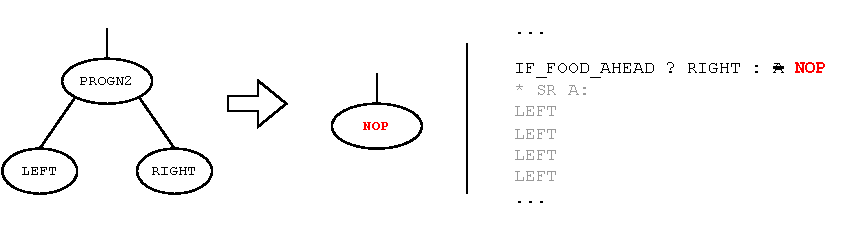
\includegraphics{obrazky-figures/optimalization.pdf}
    \caption{Příklad optimalizace výpočetního času u TGP (vlevo) a LGP}
    \label{fig:optimalization}
\end{figure}

\noindent Otázkou zůstává, zdali takové vylepšení aplikovat jen na konečné řešení nebo i v průběhu generací. Zde by mohlo docházet ke ztrátě genetického materiálu.

\section{Shrnutí dosažených výsledků}
V~rámci experimentování bylo provedeno několik vyšších stovek a nižších tisíců testů, které měly za úkol ověřit vylepšení a následně porovnat obě varianty GP. U~některých vylepšeních byl pokrok velice znatelný, u~jiných zase méně.
Experimentování započalo nejprve testováním vylepšení lineárního GP, kde byly získány velice příznivé výsledky, jež napomohly k~získání většího počtu řešení za lepší čas.
V~rámci testování selekčních metod nebylo nalezeno žádného většího výkyvu, které by jasně preferoval některou z~metod k~řešení problému Langtonova mravence oproti jiným. Všechny tři metody -- turnajová, ruleta i ranking jsou vhodné pro řešení této úlohy.
Následně proběhlo rozsáhlé hledání tří parametrů, které významně ovlivňují chování tohoto programu. Těmi jsou velikost populace a pravděpodobnosti křížení a mutace. Postupným hledáním ideální hodnoty každého parametru, jeho následným zafixováním byly nalezeny ty nejlepší výsledky. Tyto experimenty byly vykonány jak pro stezku Santa Fe, tak i náhodnou stezku, kde již sice nebyly výsledky zas až tak příznivé, ale šel zde alespoň v~pozdějších fází experimentování pozorovatelný rozdíl na základě různých parametrů a získaných řešení.
S~výsledky z~literatury proběhlo krátké srovnání s~náhodně vybranými výsledky obou implementovaných variant GP. Konvergenční křivky obou variant stromového GP vyznačovaly velkou podobnost, zatímco lineární se skrz svou povahu a~ reprezentaci chovalo velice odlišně.
Poté proběhla komplexní analýza opět výše třech zmíněných parametrů na vybrané stezce o~trochu menší velikosti, kde se na základě vybraných hodnot pro všechny tyto tři parametry zkoumalo chování pro všechny různé kombinace těchto parametrů. Na základě teplotní mapy zobrazující mediány je znatelné, že nezávisle na populaci bylo dosáhnuto velmi podobných výsledků. Poté proběhlo hlubší porovnání těchto dvou variant GP, jež ukázalo, že lineární GP je se osvědčilo jako mnohem lepší nástroj řešení této úlohy. Na závěr se uskutečnilo porovnání dvou vybraných variant křížení u stromového GP, které prokázalo, že ačkoliv komplexnější varianta, která se snaží řešit \emph{bloat}, si s úlohou poradila lépe, tak oproti jednodušší variantě trpí náročností při vyhodnocování těchto operací.

\section{Možnosti reálné aplikace úlohy}
Na základě zveřejněného článku v~roce 2022 společností Rohlik.cz~\cite{rohlik}, zabývající se internetovým prodejem zboží, zejména potravin, a jejich doručením, byl představen nový systém pro vychystávání objednávek v~logistickém centru. Tento systém pracuje s~dvojdimenzionální mřížkou, ve které jedna buňka reprezentuje objednávku zákazníka. Po této mřížce se pohybují roboti, kteří skládají zboží do objednávek. Analogicky by se dal tento problém namapovat s~menšími modifikacemi na úlohu Langtonova mravence. 

Jistě se ale najde i spousta dalších aplikací o~kterých ale zatím ještě není známo. Například se změnou dvojdimenzionální mřížky, jež by se nahradila uzly, které by mohly například představovat silniční křižovatky, a ty byly navzájem spojené cestami, čímž by se například dokázal problém ještě více adaptovat na logistické odvětví. Tyto cesty spojující uzly by mohly obsahovat nějaké parametry, mít nějakou prioritu, čímž by se opět zvětšil prohledávací prostor možných řešení a šlo by tak ověřit adaptace tohoto algoritmu na složitější podmínky.


\chapter{Závěr}\label{ch:8}
Na počátku této bakalářské práce byla nejprve představena a vysvětlena varianta stromového GP, včetně konceptů použitelných i pro ostatní varianty a v neposlední řadě taktéž stručný úvod do její historie. Následně ke konci první kapitoly proběhlo krátké srovnání s~dalšími evolučními algoritmy. Rovněž analogicky bylo popsáno v následující druhé kapitole i lineární GP. Poté byly prezentovány různé aplikace GP, od těch nejzákladnějších, jež jsou lehce pochopitelné a jsou často používány pro demonstraci této techniky, tak v neposlední řadě bylo taktéž zmíněno pár komplexnějších a zajímavějších aplikací. Mimoto bylo rovněž pojednáno o~výzkumu a pokroku v~problematice GP jako takové. V druhé polovině bakalářské práce byla prezentována úloha Langtonova umělého mravence, jež představuje abstraktní matematický model pohybujícího se mravence po dvojdimenzionální mřížce pomocí definované sady pravidel, který následně sloužil k~porovnání výše zmíněných variant GP.

Samotná implementace byla realizována téměř od základu v~jazyce Python. Pouze u~první varianty GP s využitím již existujícího jednoduchého programu. První grafická reprezentace úlohy byla implementována za pomocí ASCII Artu. Později s~využitím knihoven matplotlib a imageio byla vytvořena pokročilejší vizualizace generující řešení ve formátu \emph{gif}, který je snadněji prezentovatelnější. V~praktické části proběhla komplexní analýza a následné statistické vyhodnocení několika různých instancí problému s odlišným nastavením. To zahrnovalo experimentování s různými parametry za dosáhnutím co nejlepších výsledků, experimenty s vylepšeními, porovnání různých variačních operátorů v~rámci jednotlivých variant GP, srovnání s~výsledky dostupnými v~literatuře a taktéž srovnání obou variant GP. 

Získané výsledky z experimentů vyústily v~závěr, že lineární GP se prokázalo jako mnohem efektivnější nástroj k~řešení této úlohy, než tradiční stromové GP, které je na tuto úlohu aplikováno v~literatuře. Dále bylo zjištěno, že operátor mutace se jeví jako mnohem důležitější a mající pozitivnější vliv na získaná řešení než operátor křížení. Ke konci práce byly zmíněny další rozšíření či optimalizace a taktéž reálné využití na nichž bylo možné tento problém následně aplikovat.

  \fi
  
  % Kompilace po částech (viz výše, nutno odkomentovat a zakomentovat input výše)
  % Compilation piecewise (see above, it is necessary to uncomment it and comment out input above)
  %\subfile{chapters/projekt-01-uvod-introduction}
  % ...
  %\subfile{chapters/projekt-05-zaver-conclusion}

  % Pouzita literatura / Bibliography
  % ----------------------------------------------
\ifslovak
  \makeatletter
  \def\@openbib@code{\addcontentsline{toc}{chapter}{Literatúra}}
  \makeatother
  \bibliographystyle{bib-styles/Pysny/skplain}
\else
  \ifczech
    \makeatletter
    \def\@openbib@code{\addcontentsline{toc}{chapter}{Literatura}}
    \makeatother
    \bibliographystyle{bib-styles/Pysny/czplain}
  \else 
    \makeatletter
    \def\@openbib@code{\addcontentsline{toc}{chapter}{Bibliography}}
    \makeatother
    \bibliographystyle{bib-styles/Pysny/enplain}
  %  \bibliographystyle{alpha}
  \fi
\fi
  \begin{flushleft}
  \bibliography{p02-literatura}
  \end{flushleft}

  % vynechani stranky v oboustrannem rezimu
  % Skip the page in the two-sided mode
  \iftwoside
    \cleardoublepage
  \fi

  % Prilohy / Appendices
  % ---------------------------------------------
  \appendix
\ifczech
  \renewcommand{\appendixpagename}{Přílohy}
  \renewcommand{\appendixtocname}{Přílohy}
  \renewcommand{\appendixname}{Příloha}
\fi
\ifslovak
  \renewcommand{\appendixpagename}{Prílohy}
  \renewcommand{\appendixtocname}{Prílohy}
  \renewcommand{\appendixname}{Príloha}
\fi
%  \appendixpage

% vynechani stranky v oboustrannem rezimu
% Skip the page in the two-sided mode
%\iftwoside
%  \cleardoublepage
%\fi
  
\ifslovak
%  \section*{Zoznam príloh}
%  \addcontentsline{toc}{section}{Zoznam príloh}
\else
  \ifczech
%    \section*{Seznam příloh}
%    \addcontentsline{toc}{section}{Seznam příloh}
  \else
%    \section*{List of Appendices}
%    \addcontentsline{toc}{section}{List of Appendices}
  \fi
\fi
  \startcontents[chapters]
  \setlength{\parskip}{0pt} 
  % seznam příloh / list of appendices
  % \printcontents[chapters]{l}{0}{\setcounter{tocdepth}{2}}
  
  \ifODSAZ
    \setlength{\parskip}{0.5\bigskipamount}
  \else
    \setlength{\parskip}{0pt}
  \fi
  
  % vynechani stranky v oboustrannem rezimu
  \iftwoside
    \cleardoublepage
  \fi
  
  % Přílohy / Appendices
  \ifenglish
    \input{projekt-30-prilohy-appendices-en}
  \else
    \chapter{Obsah přiloženého média}
\begin{itemize}
    \item \texttt{src/} -- Zdrojové soubory s TGP a LGP.
    \item \texttt{exp/} -- Získaná data z experimentování následně použitá pro grafové zobrazení. 
    \item \texttt{latex/} -- Zdrojové soubory k bakalářské práci.
    \item \texttt{README.md} -- Návod ke spuštění programu.
    \item \texttt{gp\_visualization.png} -- Ukázka vizualizace řešení.
    \item \texttt{requirements.txt} -- Knihovny a balíčky Pythonu, které je potřeba ke správnému fungování programu instalovat.
    \item \texttt{thesis.pdf} -- Bakalářská práce v souboru PDF.
    \item \texttt{thesis-print.pdf} -- Bakalářská práce určená k tisku.
\end{itemize}
  \fi
  
  % Kompilace po částech (viz výše, nutno odkomentovat)
  % Compilation piecewise (see above, it is necessary to uncomment it)
  %\subfile{projekt-30-prilohy-appendices}
  
\end{document}
